\subsection{Защита информации}
	
	\subsubsection{Аннотация}

        Курс <<Защита информации>> получил в основном негативные отзывы. 
        
        Руководствуясь результатами опроса, Совет студентов и аспирантов ФРКТ выдвигает следующие идеи по улучшению данного курса:
        \begin{enumerate}
            \item уменьшить количество рутинных вычислений и добавить больше задач, связанных с реальными кейсами и современными технологиями;
            \item пересмотреть формат курса: уменьшить количество вычислений и добавить больше задач, связанных с программированием, рассказывать про взломы методов шифрования, про нарушение безопасности, про гарантии безопасности ОС, про сетевую безопасность;
            \item донести критерии оценивания до студентов так, чтобы они были ясны им.
        \end{enumerate}

	\subsubsection{Общий отзыв студентов о курсе}

		\begin{figure}[H]
			\centering
			\begin{subfigure}[b]{0.45\textwidth}
				\centering
				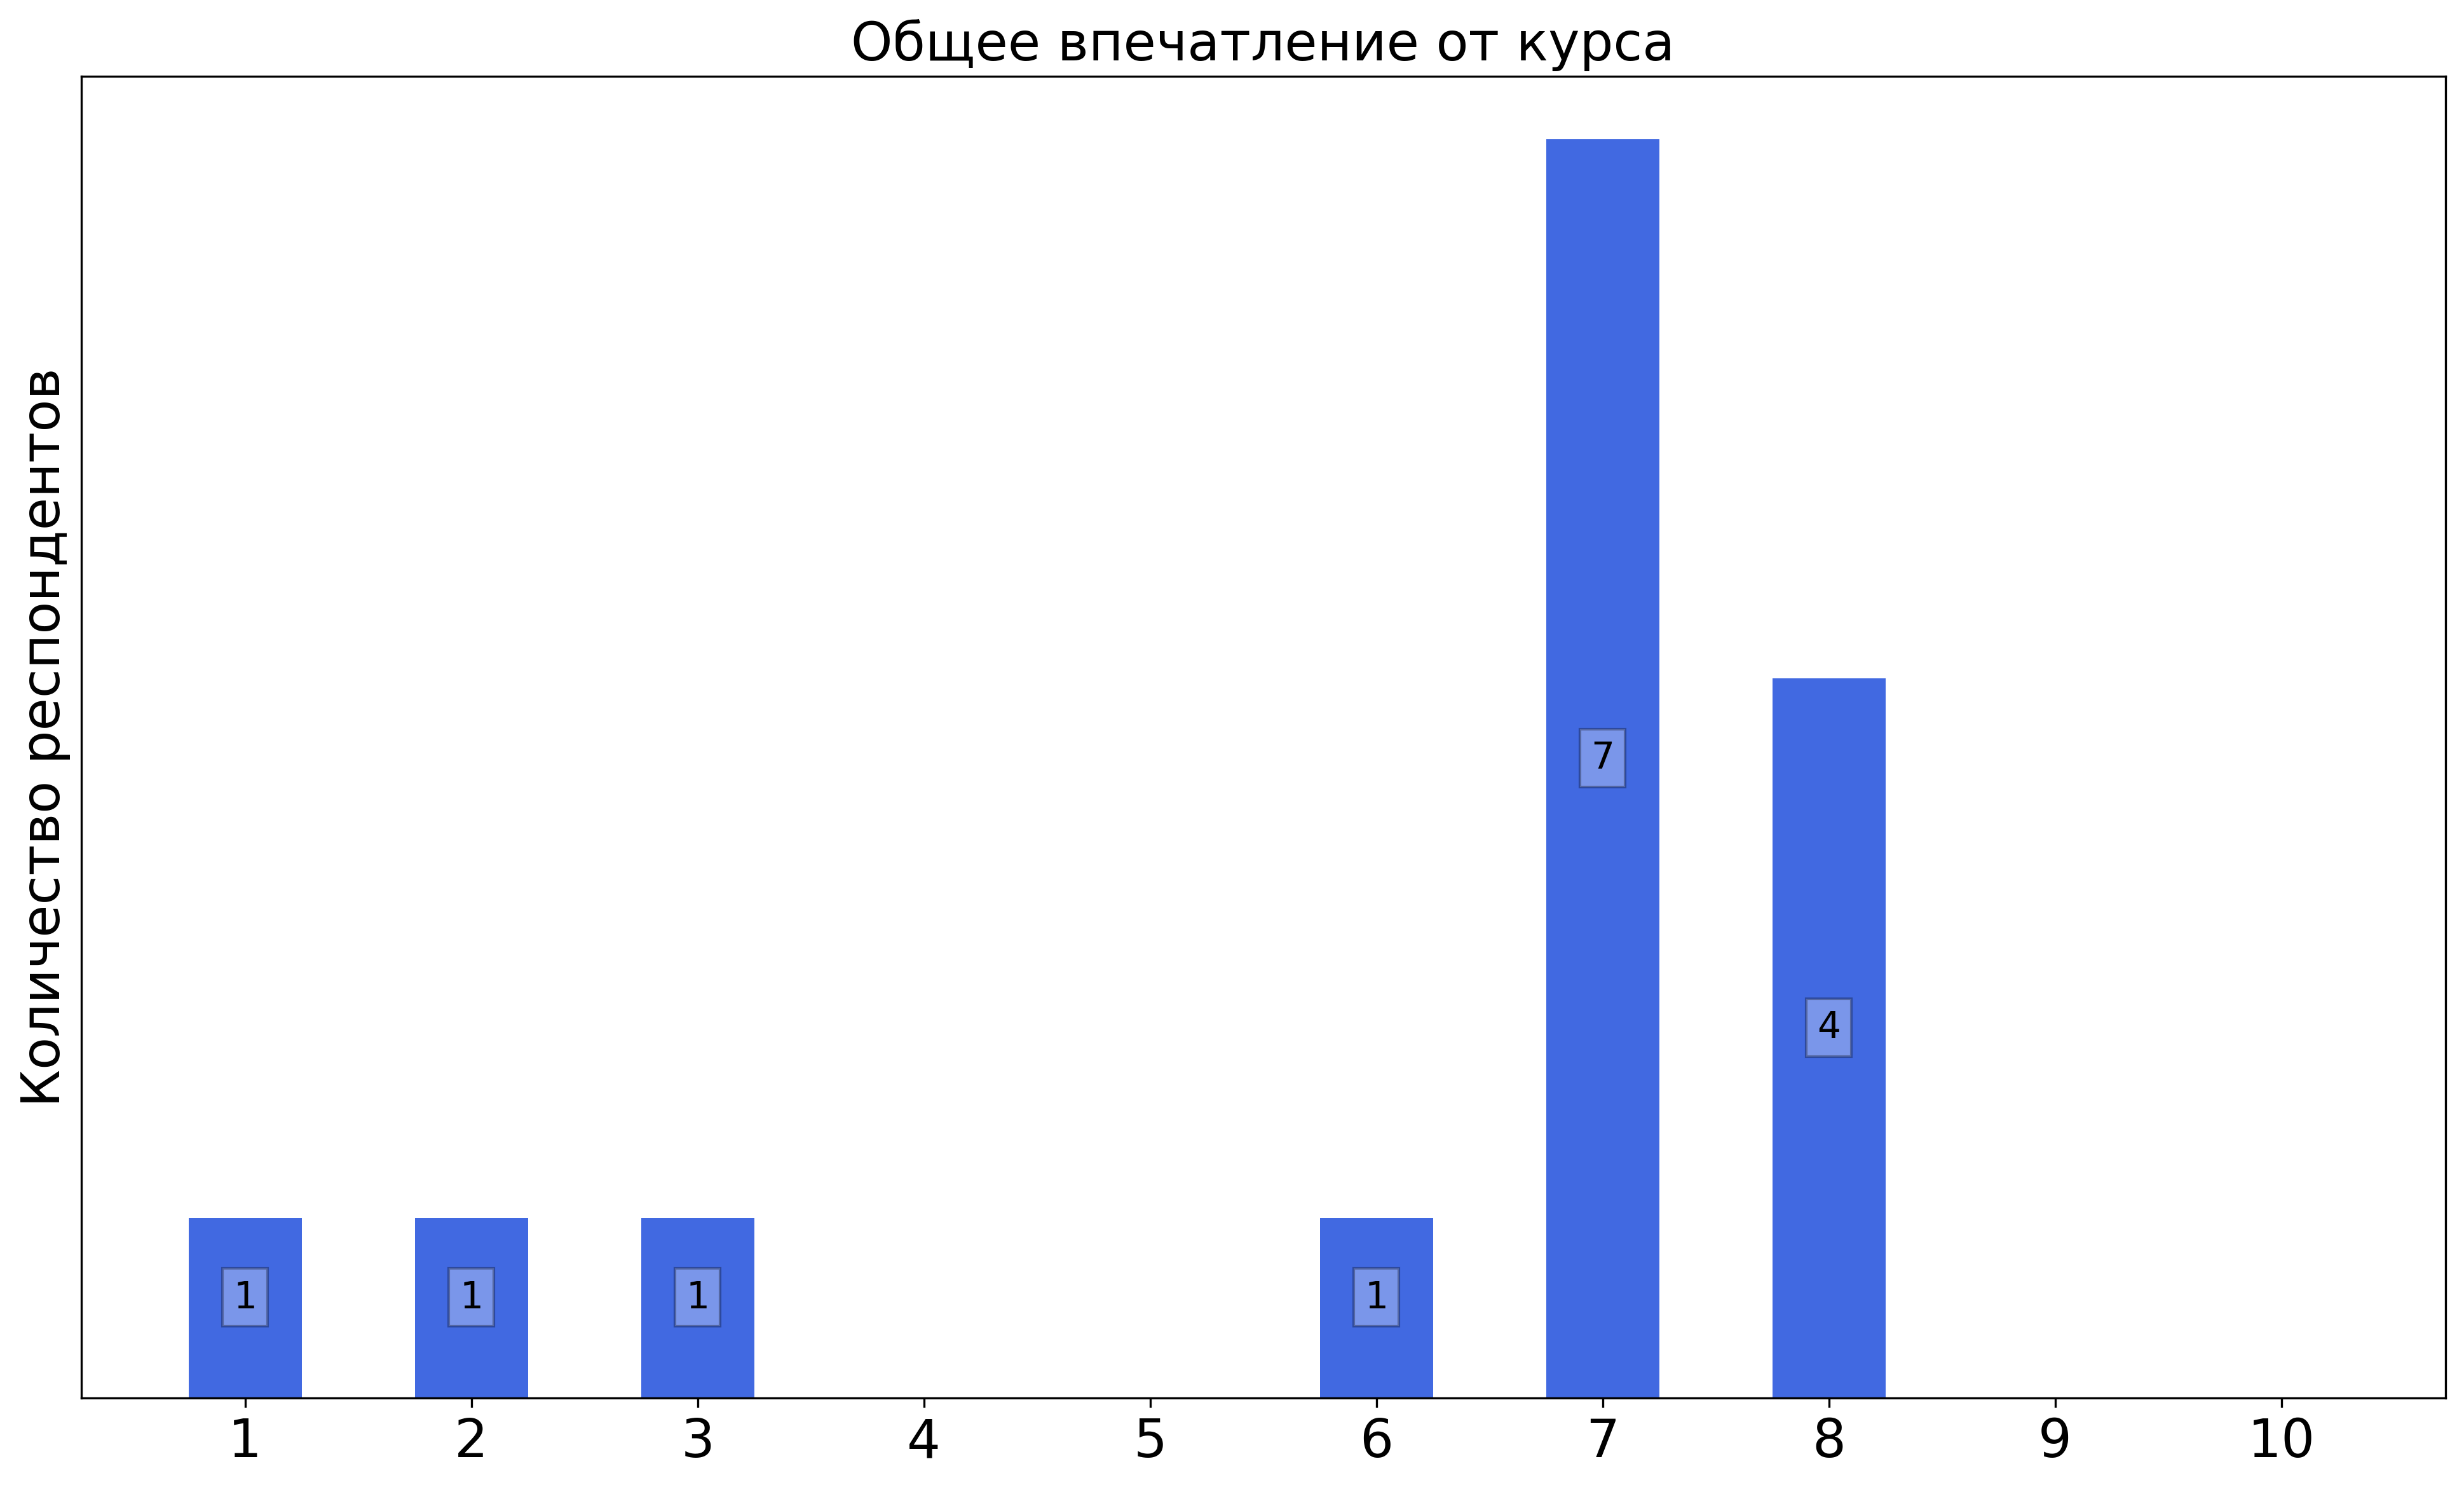
\includegraphics[width=\textwidth]{images/4 course/Защита информации/general-0.png}
			\end{subfigure}
			\begin{subfigure}[b]{0.45\textwidth}
				\centering
				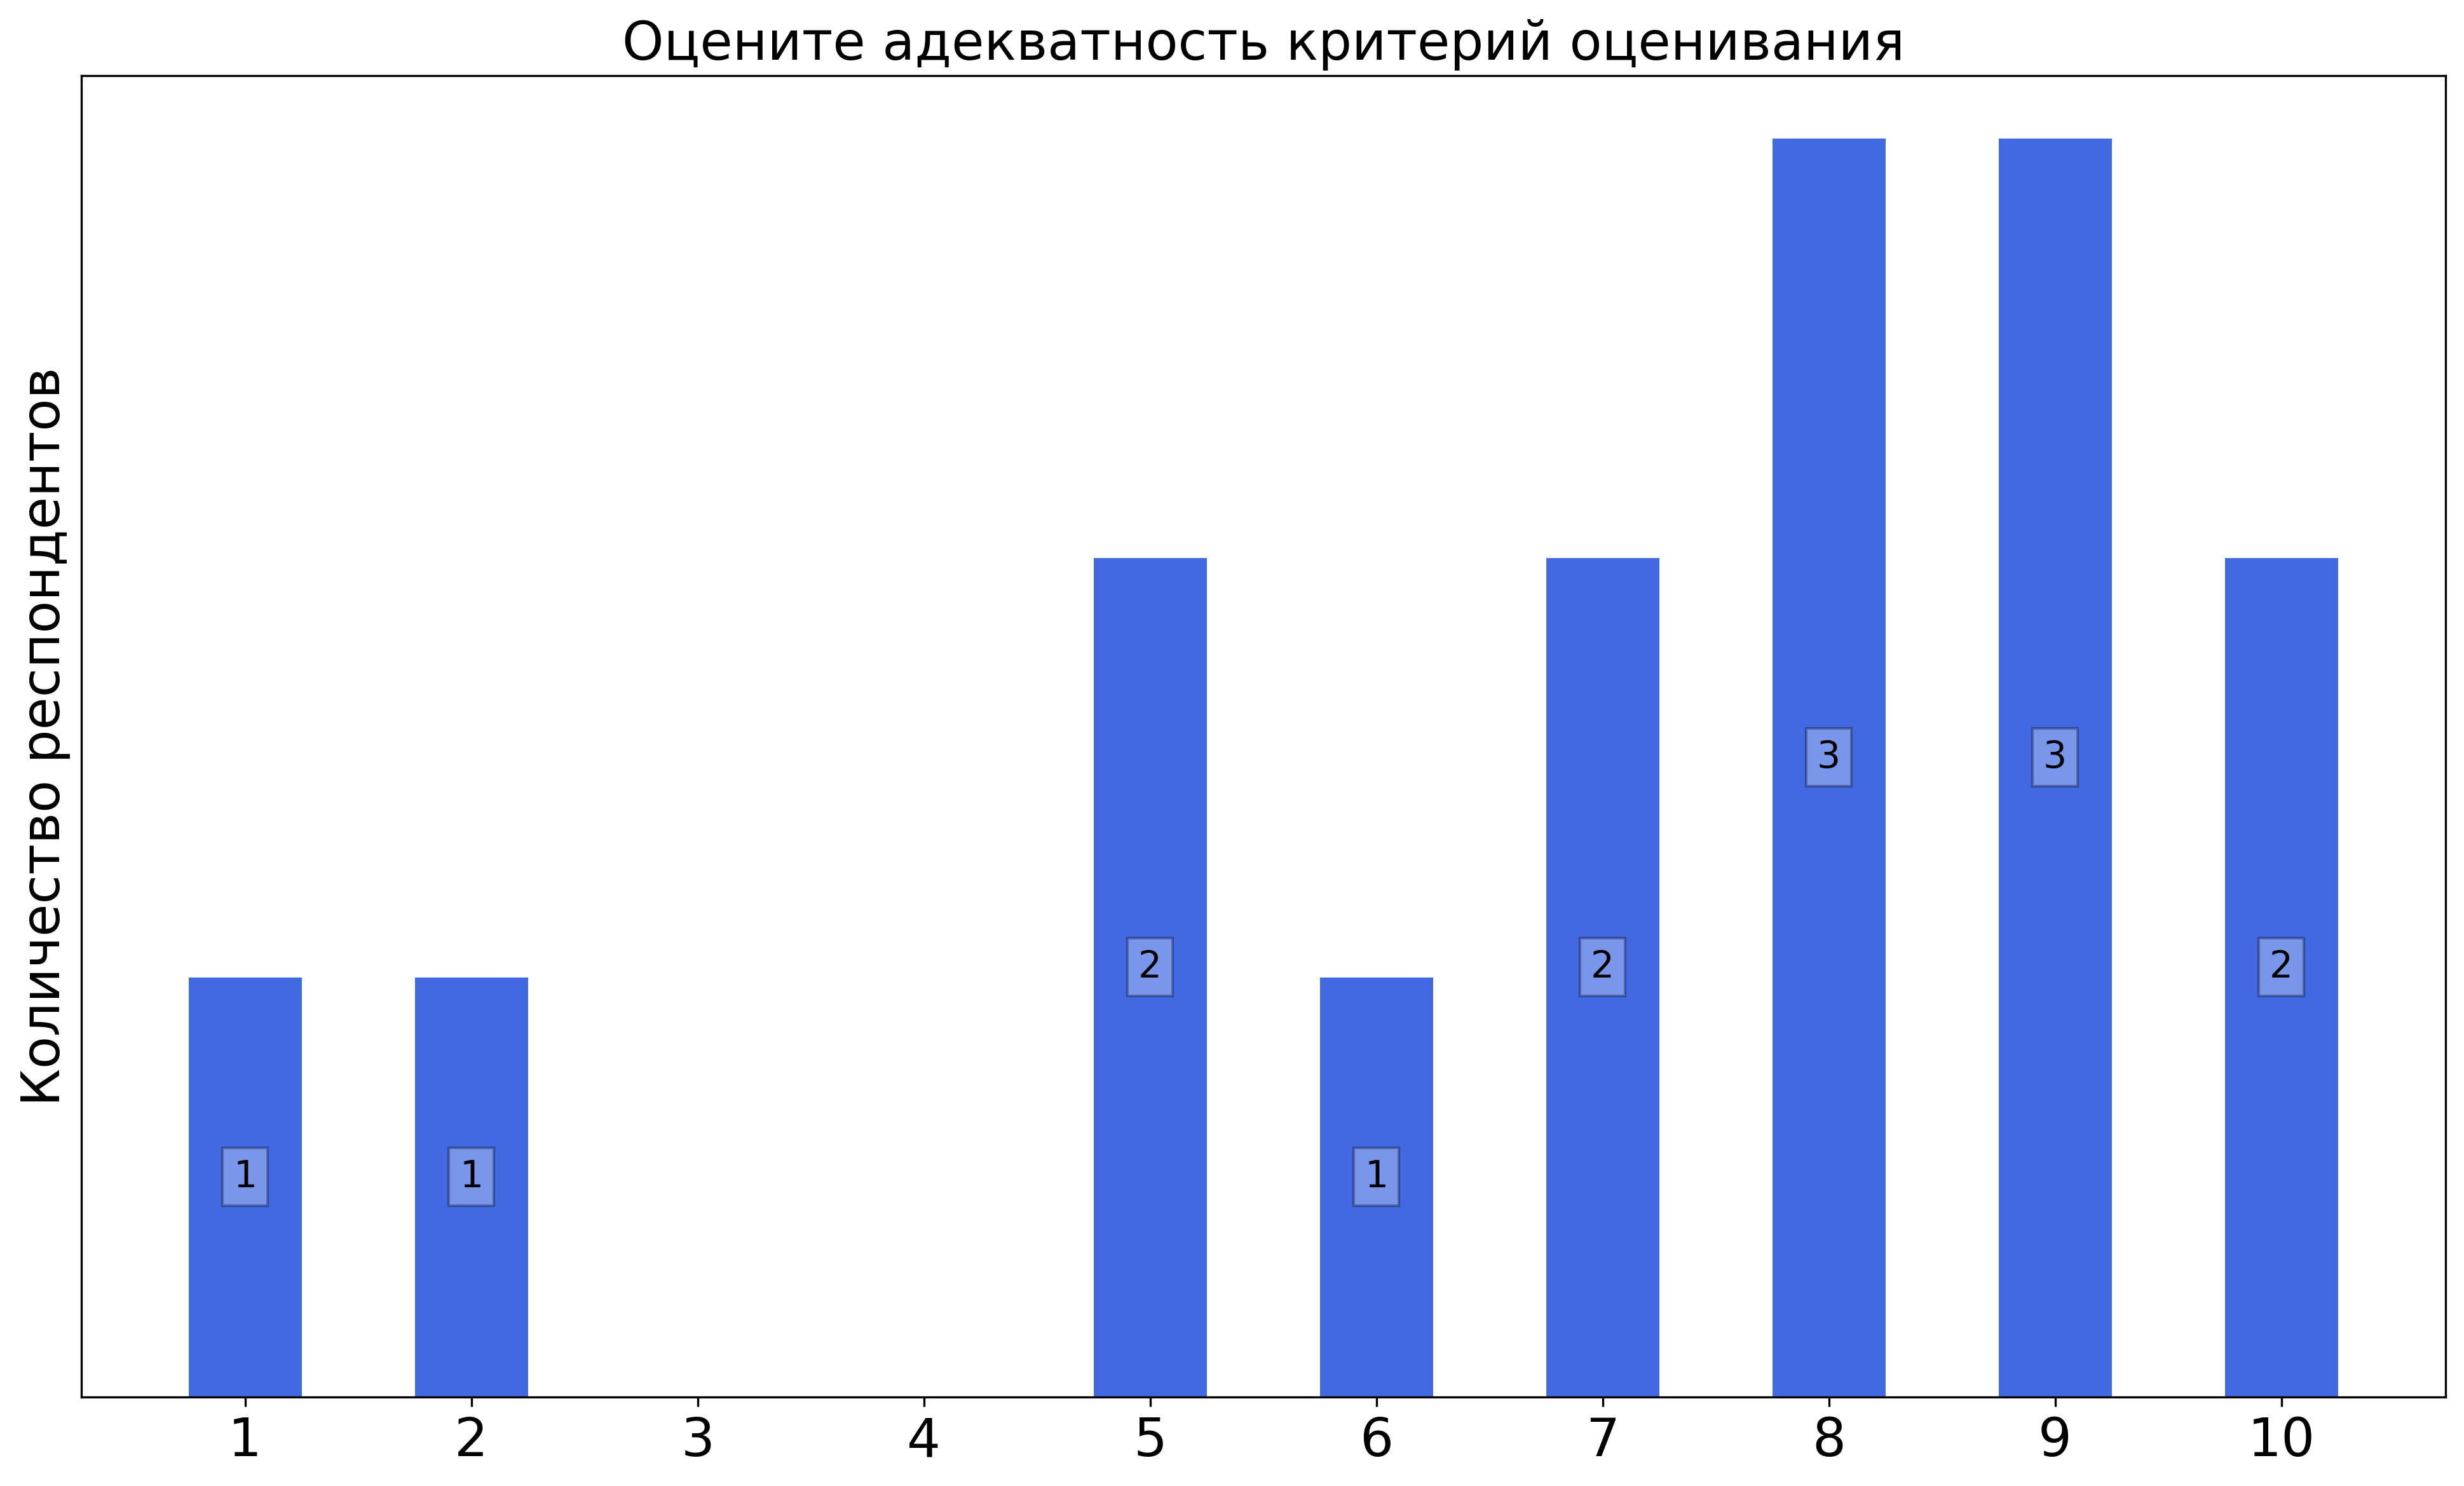
\includegraphics[width=\textwidth]{images/4 course/Защита информации/general-1.png}
			\end{subfigure}	
		\end{figure}

	\subsubsection{Материалы, использумые респондентами при изучении курса}

		\begin{figure}[H]
			\centering
			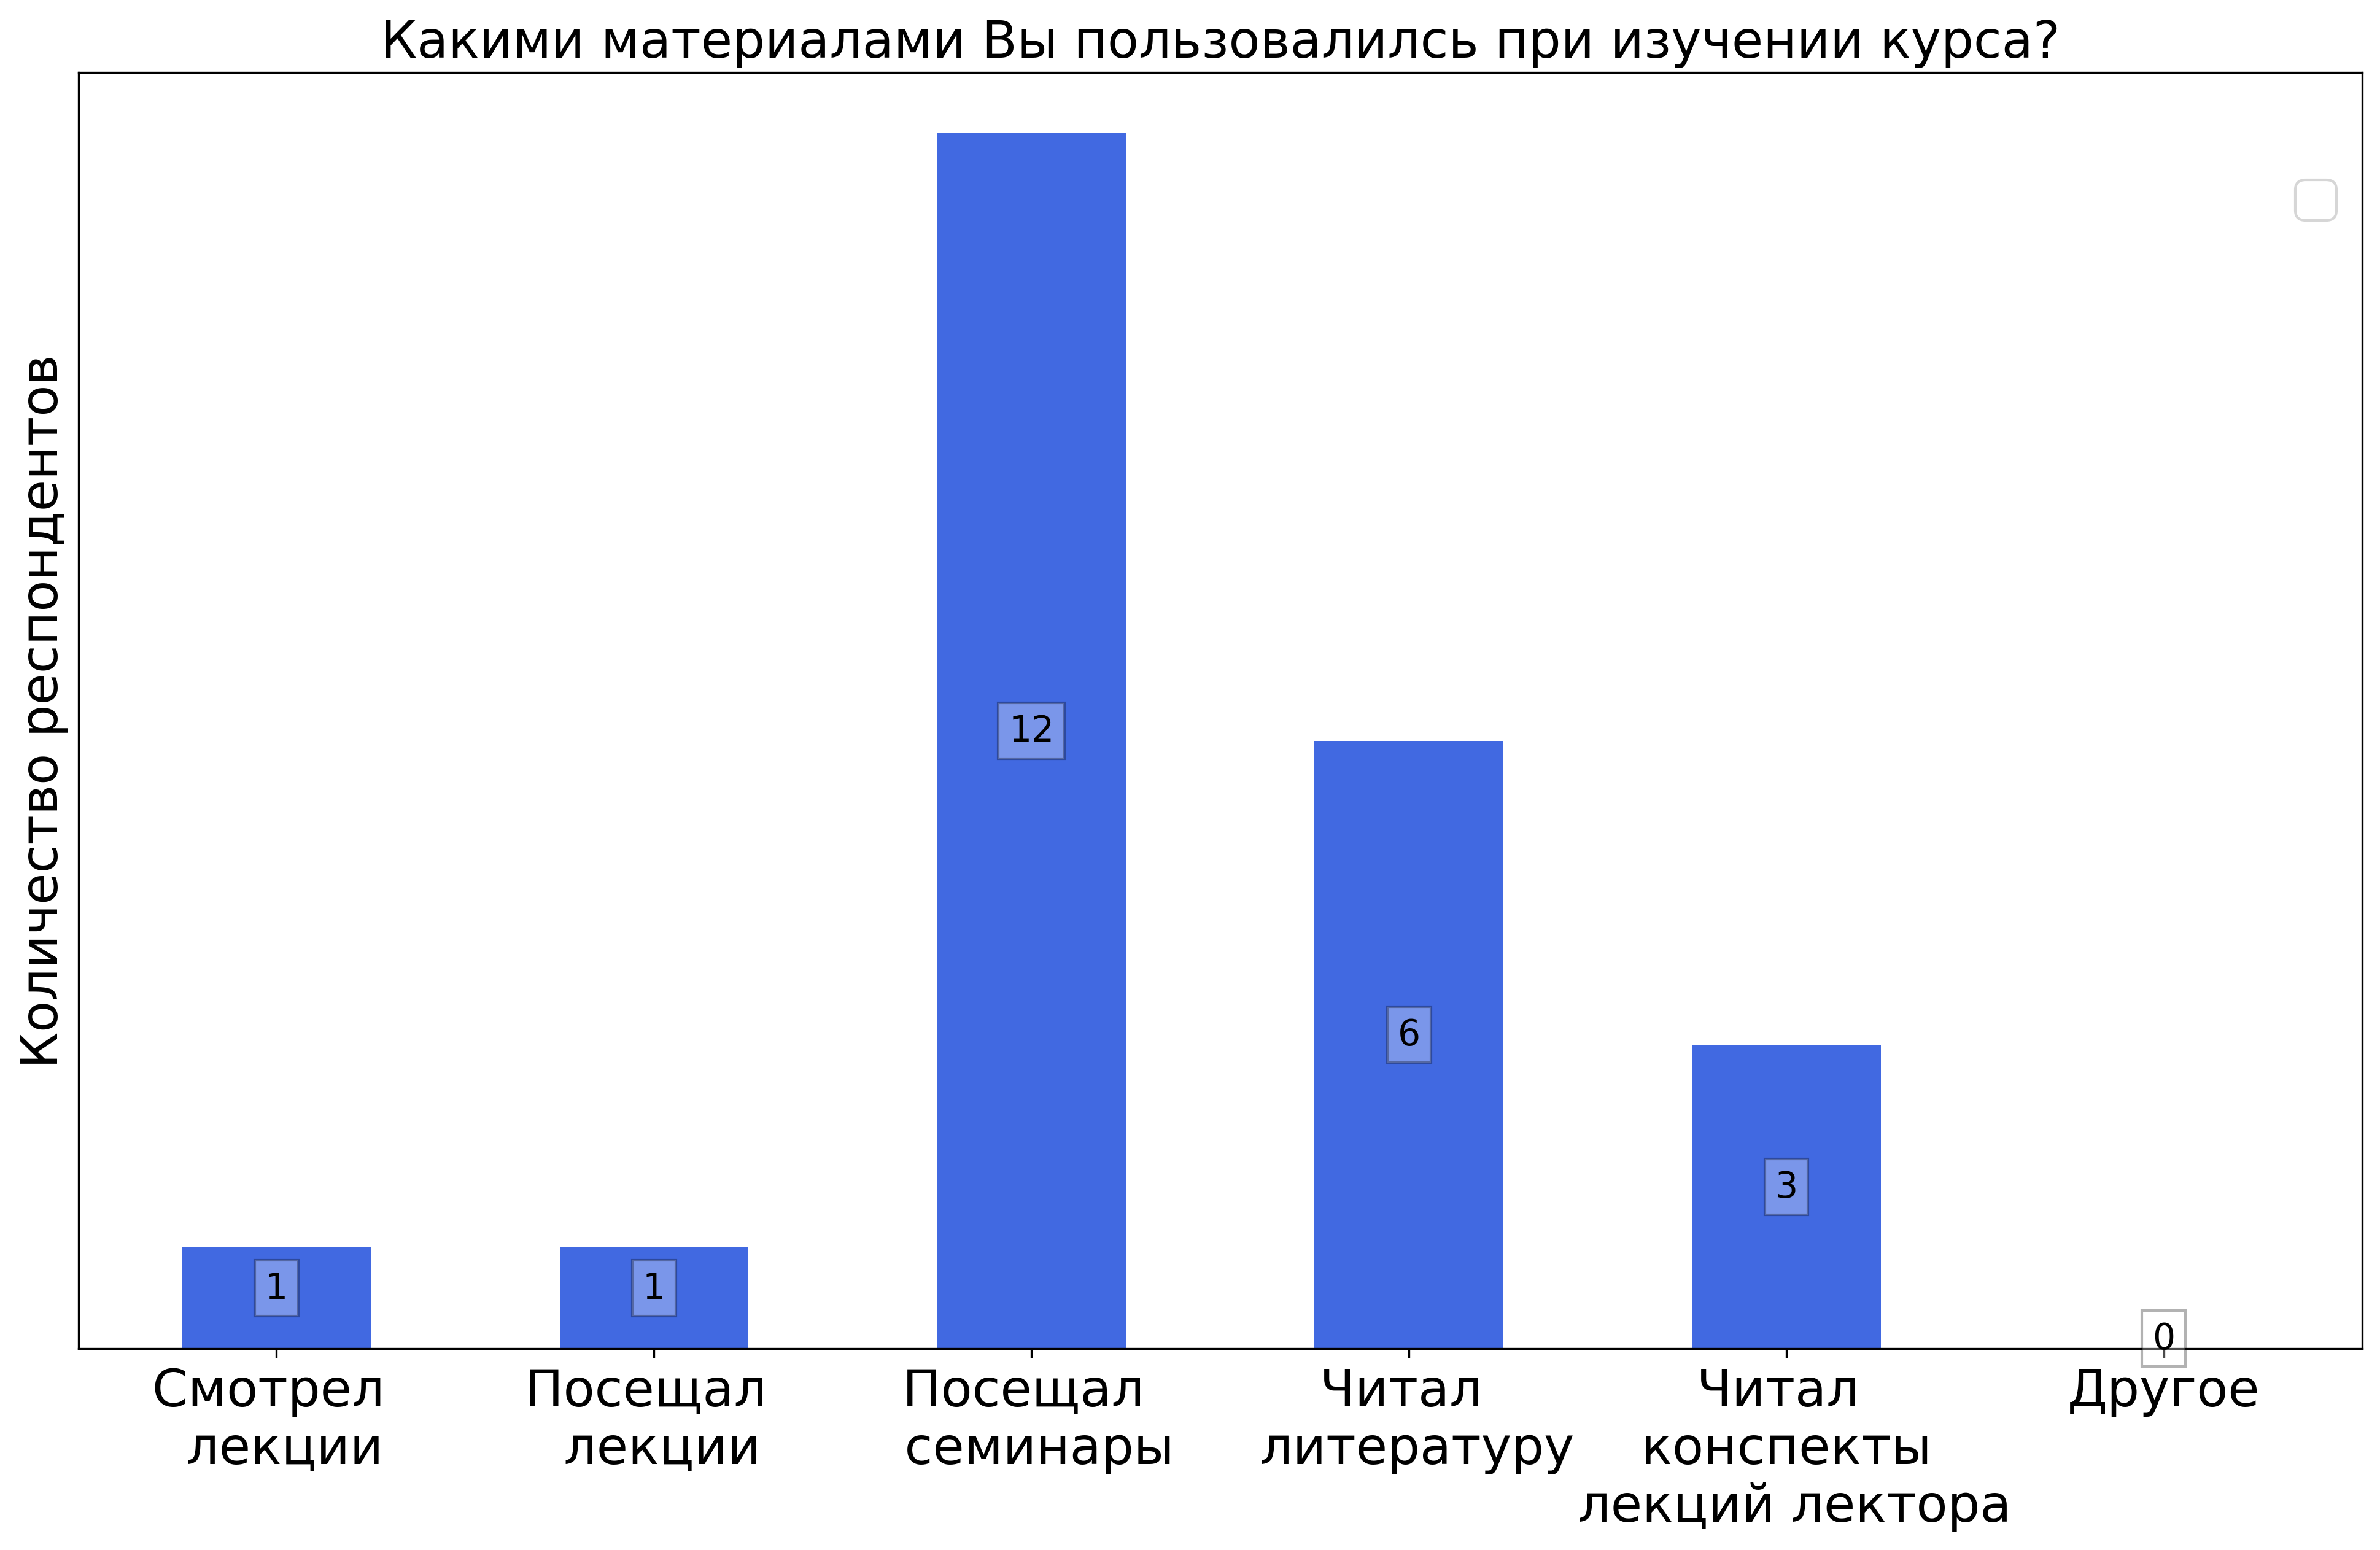
\includegraphics[width = 0.45\textwidth]{images/4 course/Защита информации/materials.png}
		\end{figure}


	\subsubsection{Отзыв студентов о лекциях. Лектор: Колыбельников А.И.}
		\begin{figure}[H]
			\centering
            \begin{subfigure}[b]{0.45\textwidth}
				\centering
				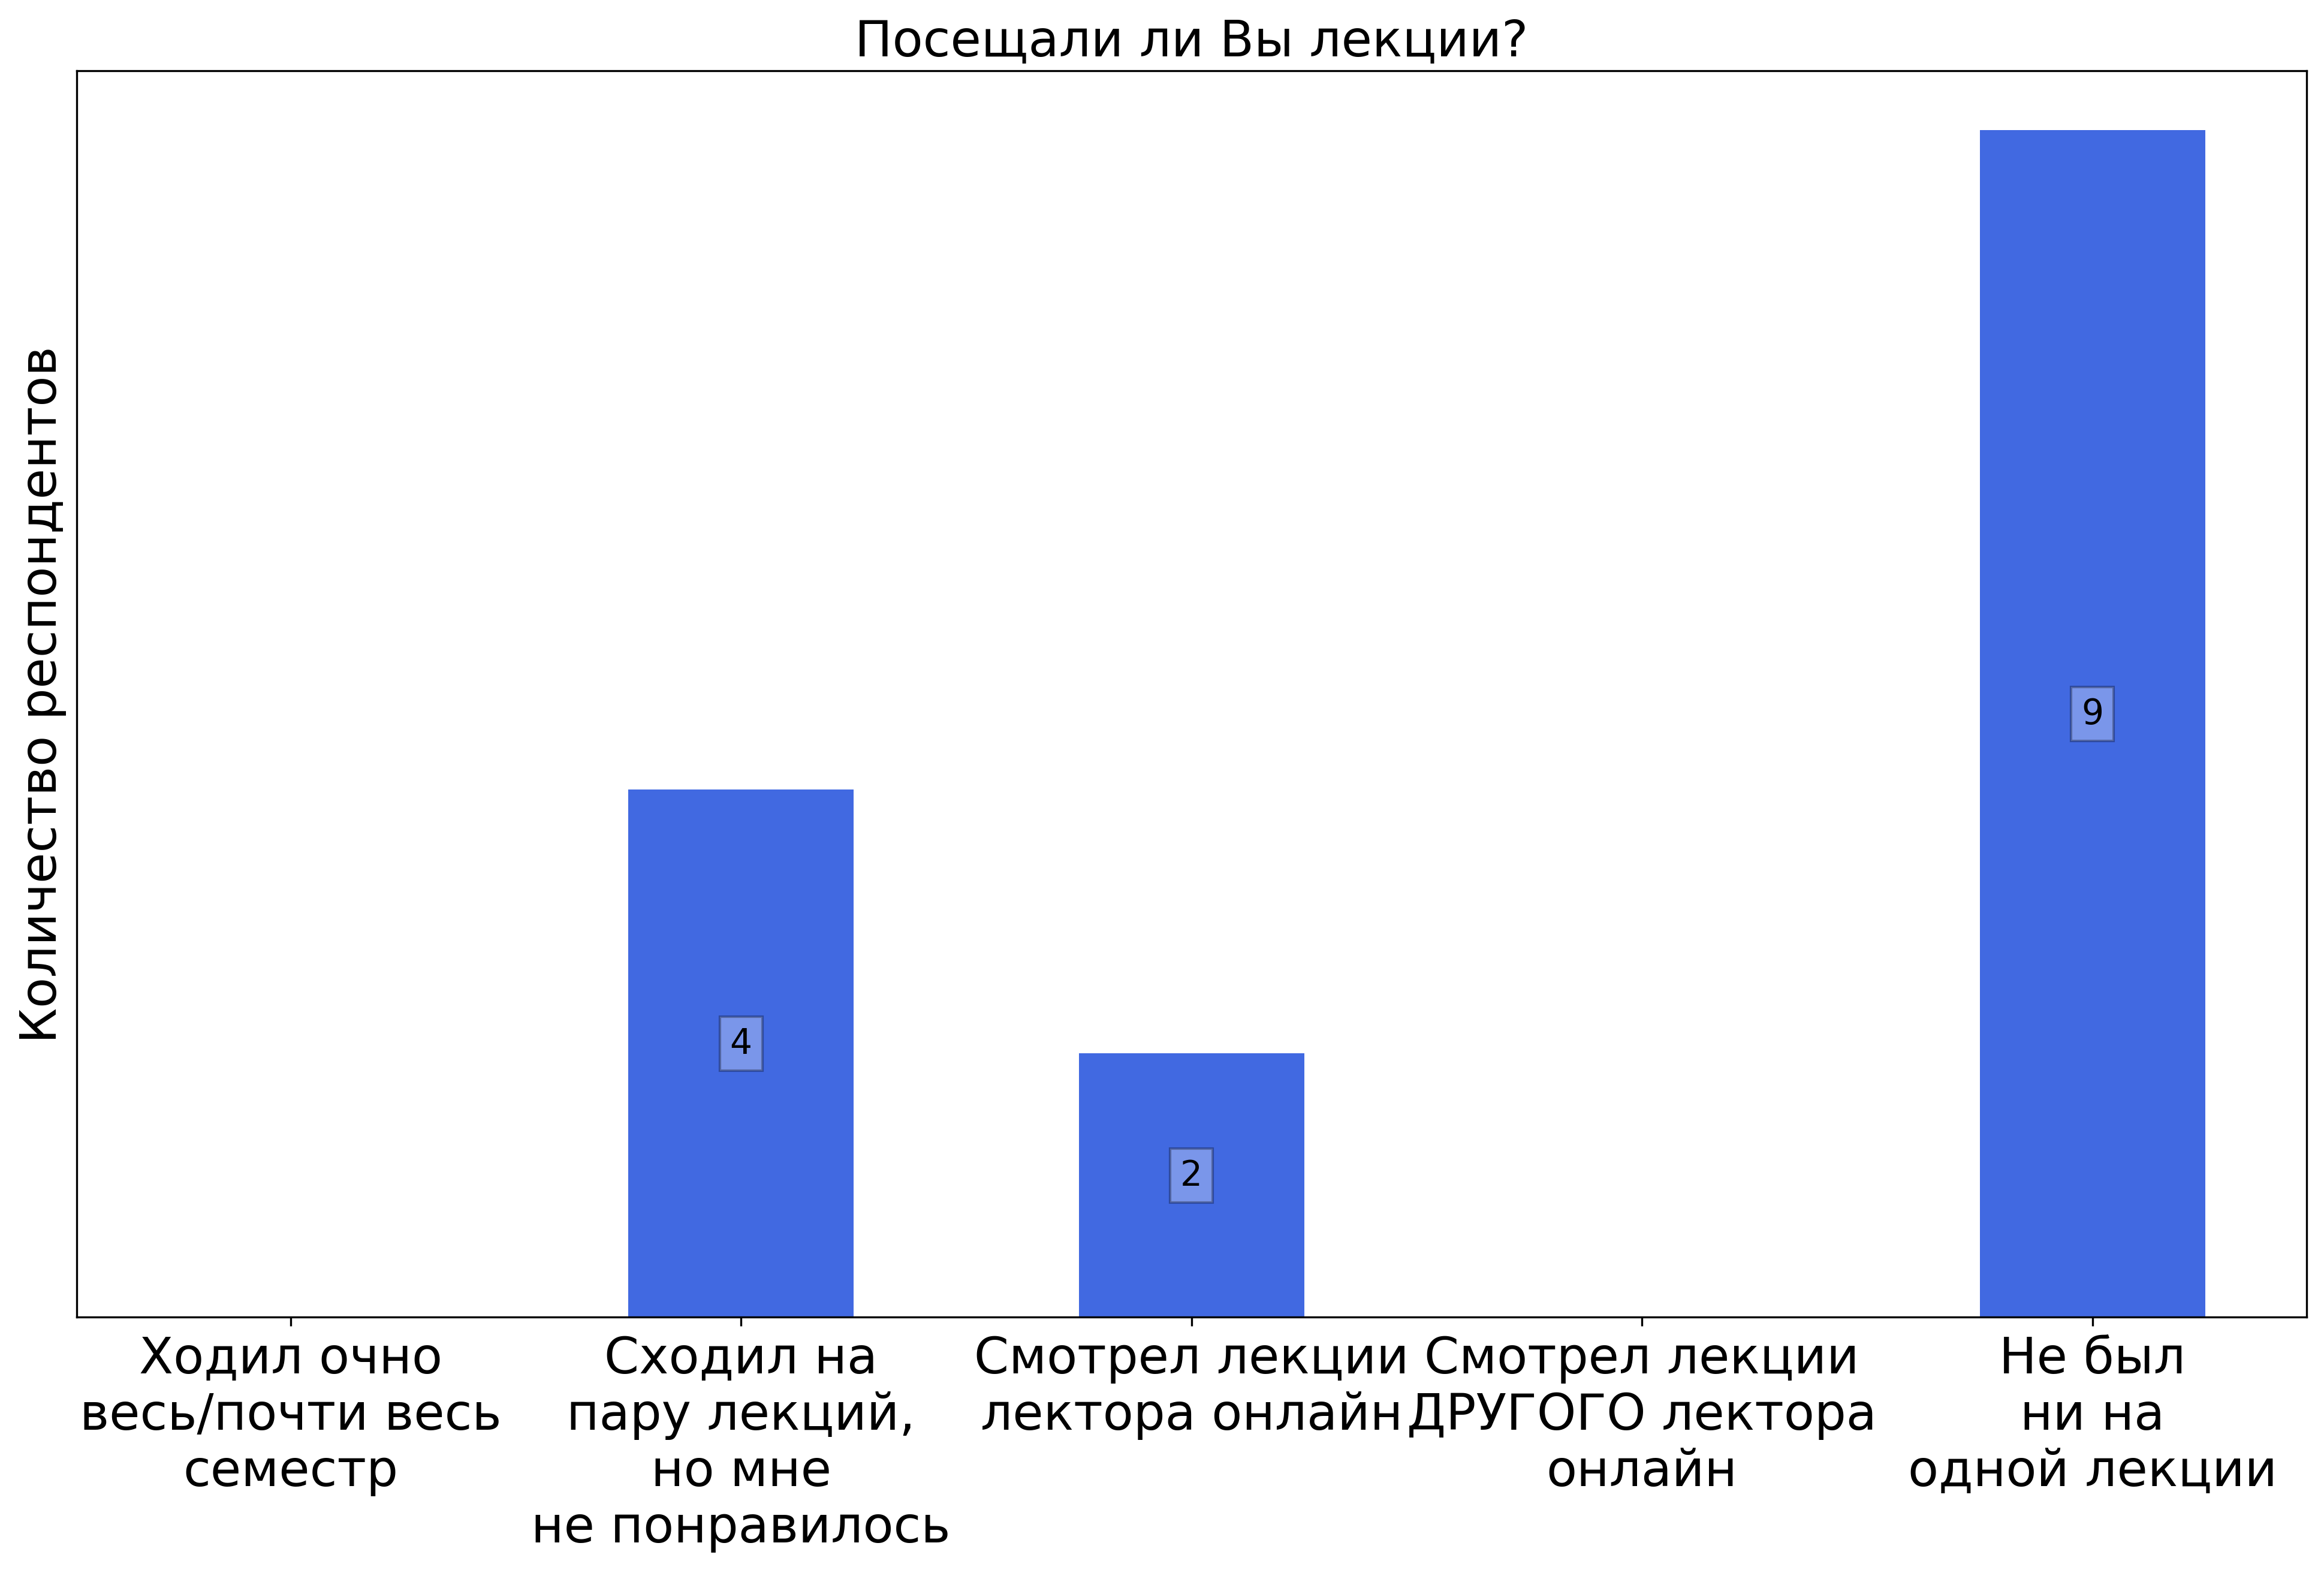
\includegraphics[width=\textwidth]{images/4 course/Защита информации/lecturer-questions-Колыбельников А.И.-0.png}
			\end{subfigure}
			\begin{subfigure}[b]{0.45\textwidth}
				\centering
				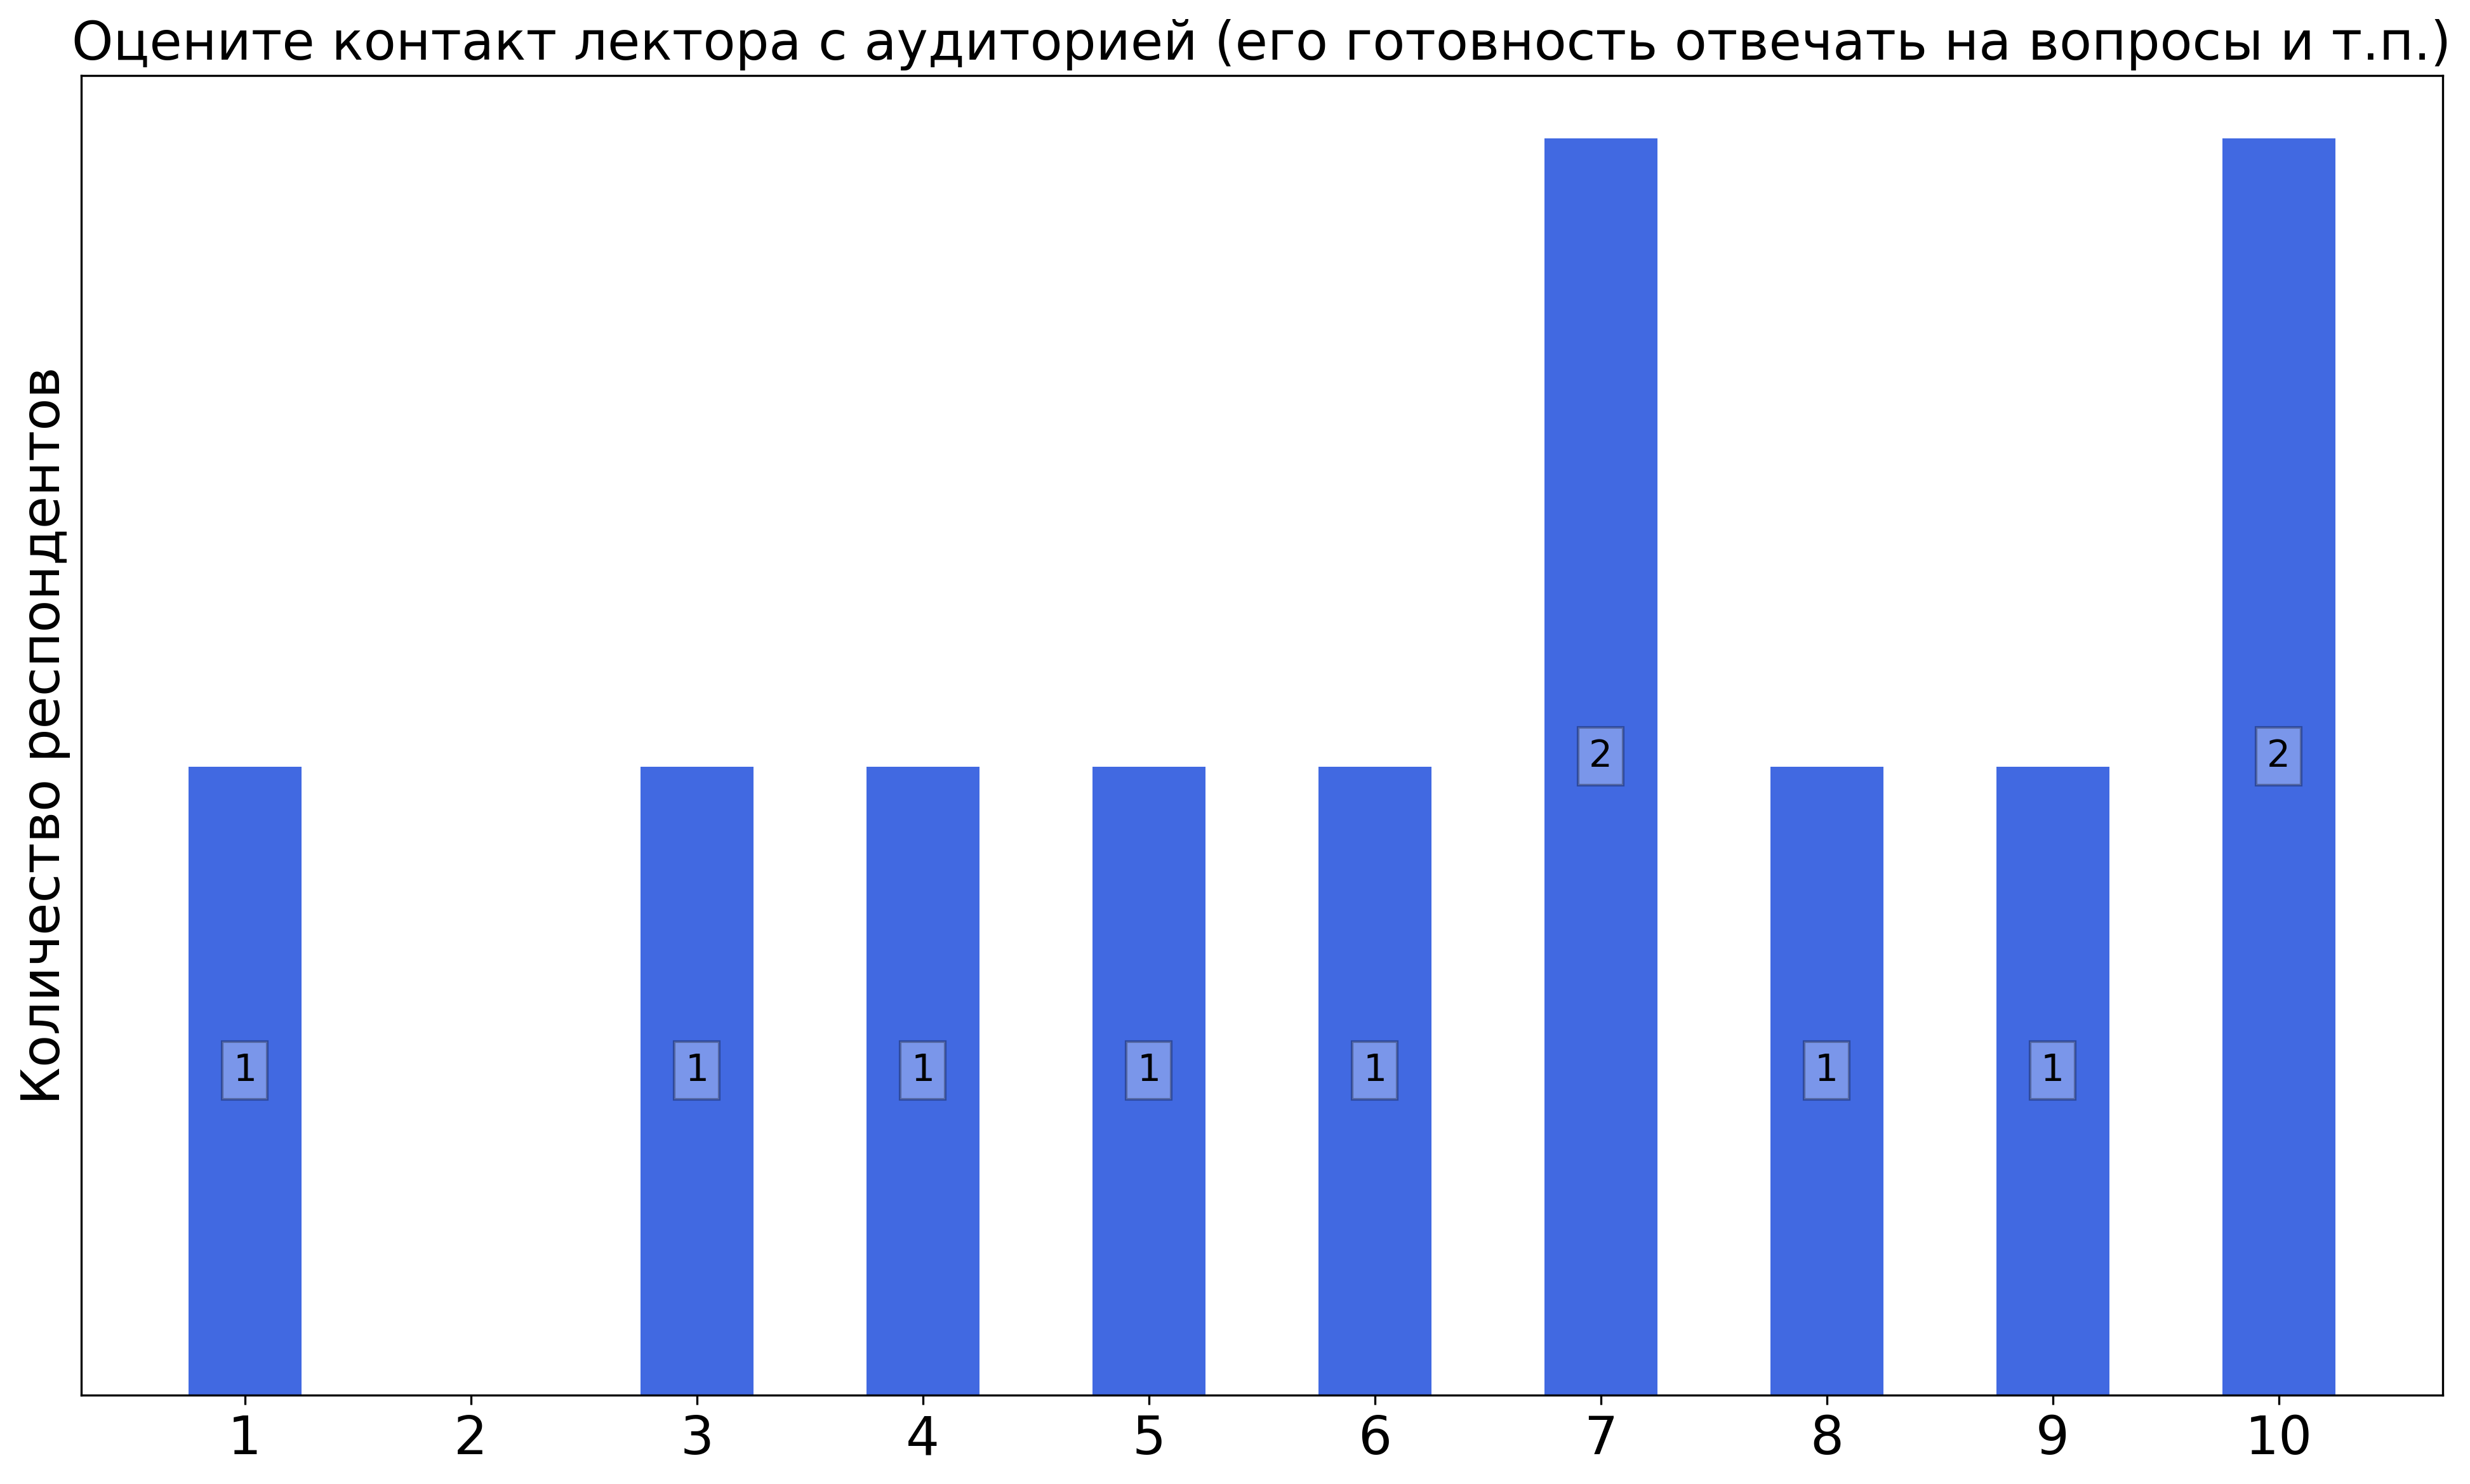
\includegraphics[width=\textwidth]{images/4 course/Защита информации/lecturer-marks-Колыбельников А.И.-0.png}
			\end{subfigure}
			\begin{subfigure}[b]{0.45\textwidth}
				\centering
				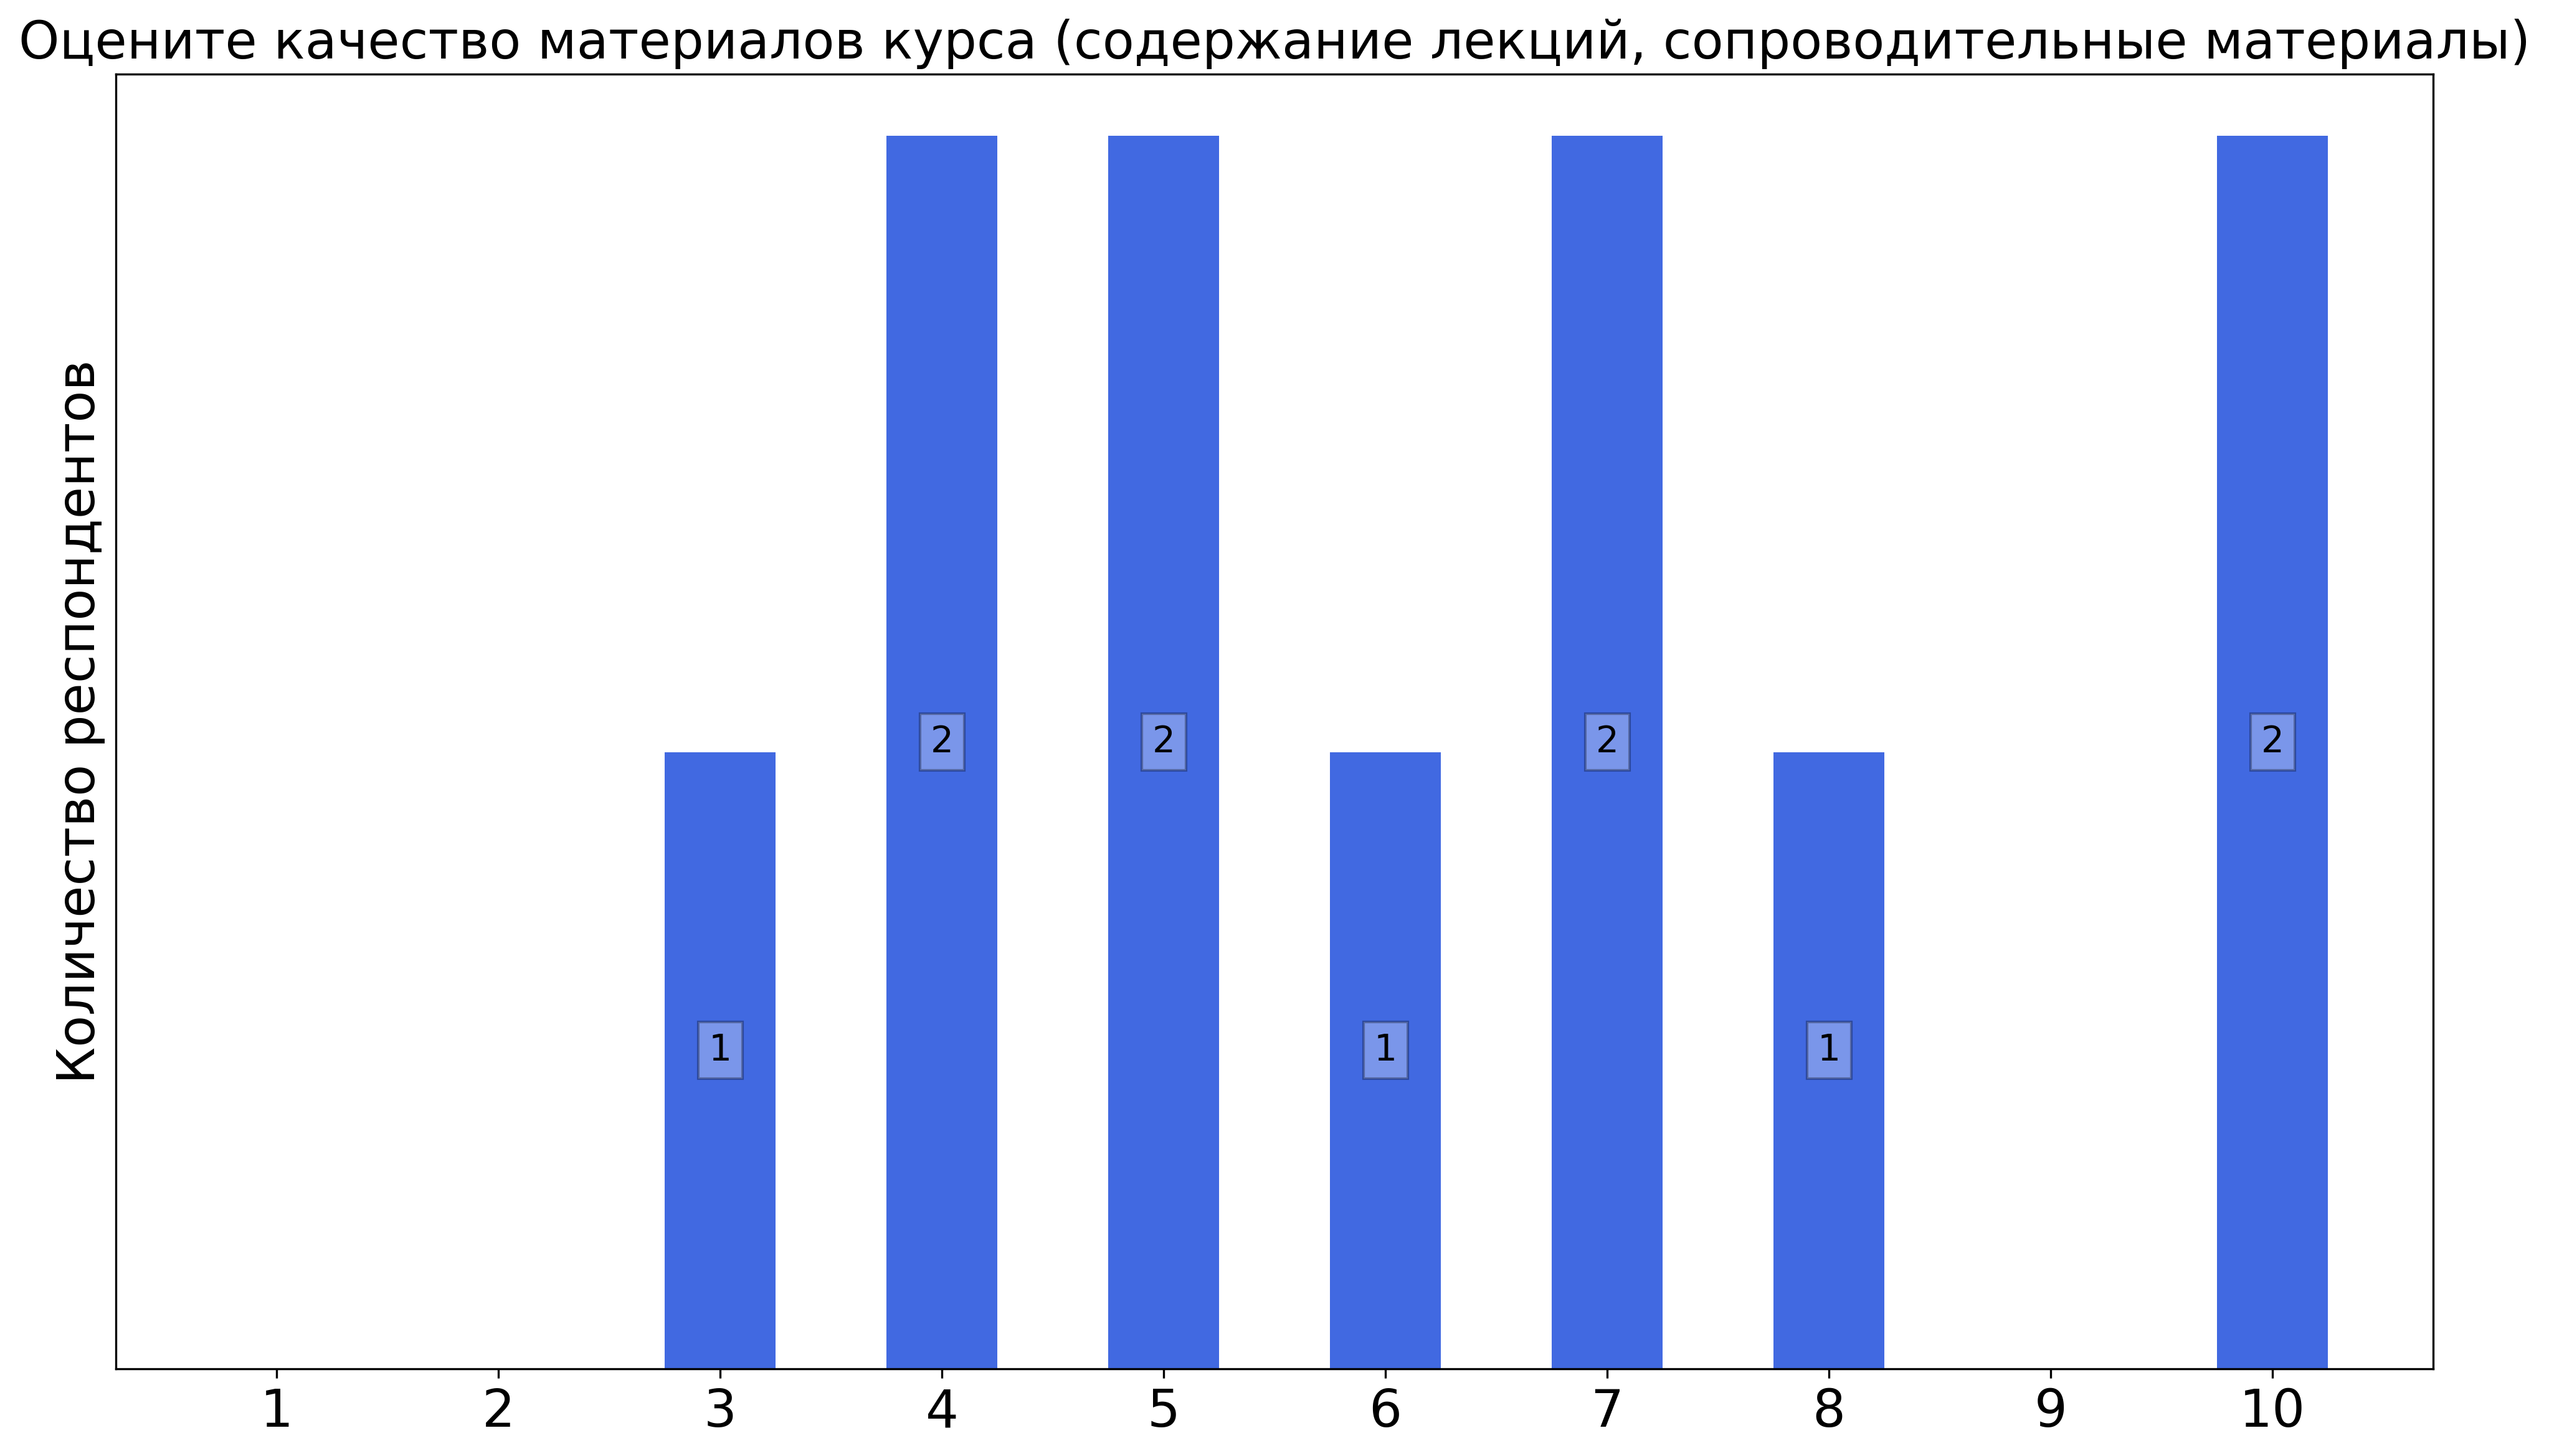
\includegraphics[width=\textwidth]{images/4 course/Защита информации/lecturer-marks-Колыбельников А.И.-1.png}
			\end{subfigure}
			\begin{subfigure}[b]{0.45\textwidth}
				\centering
				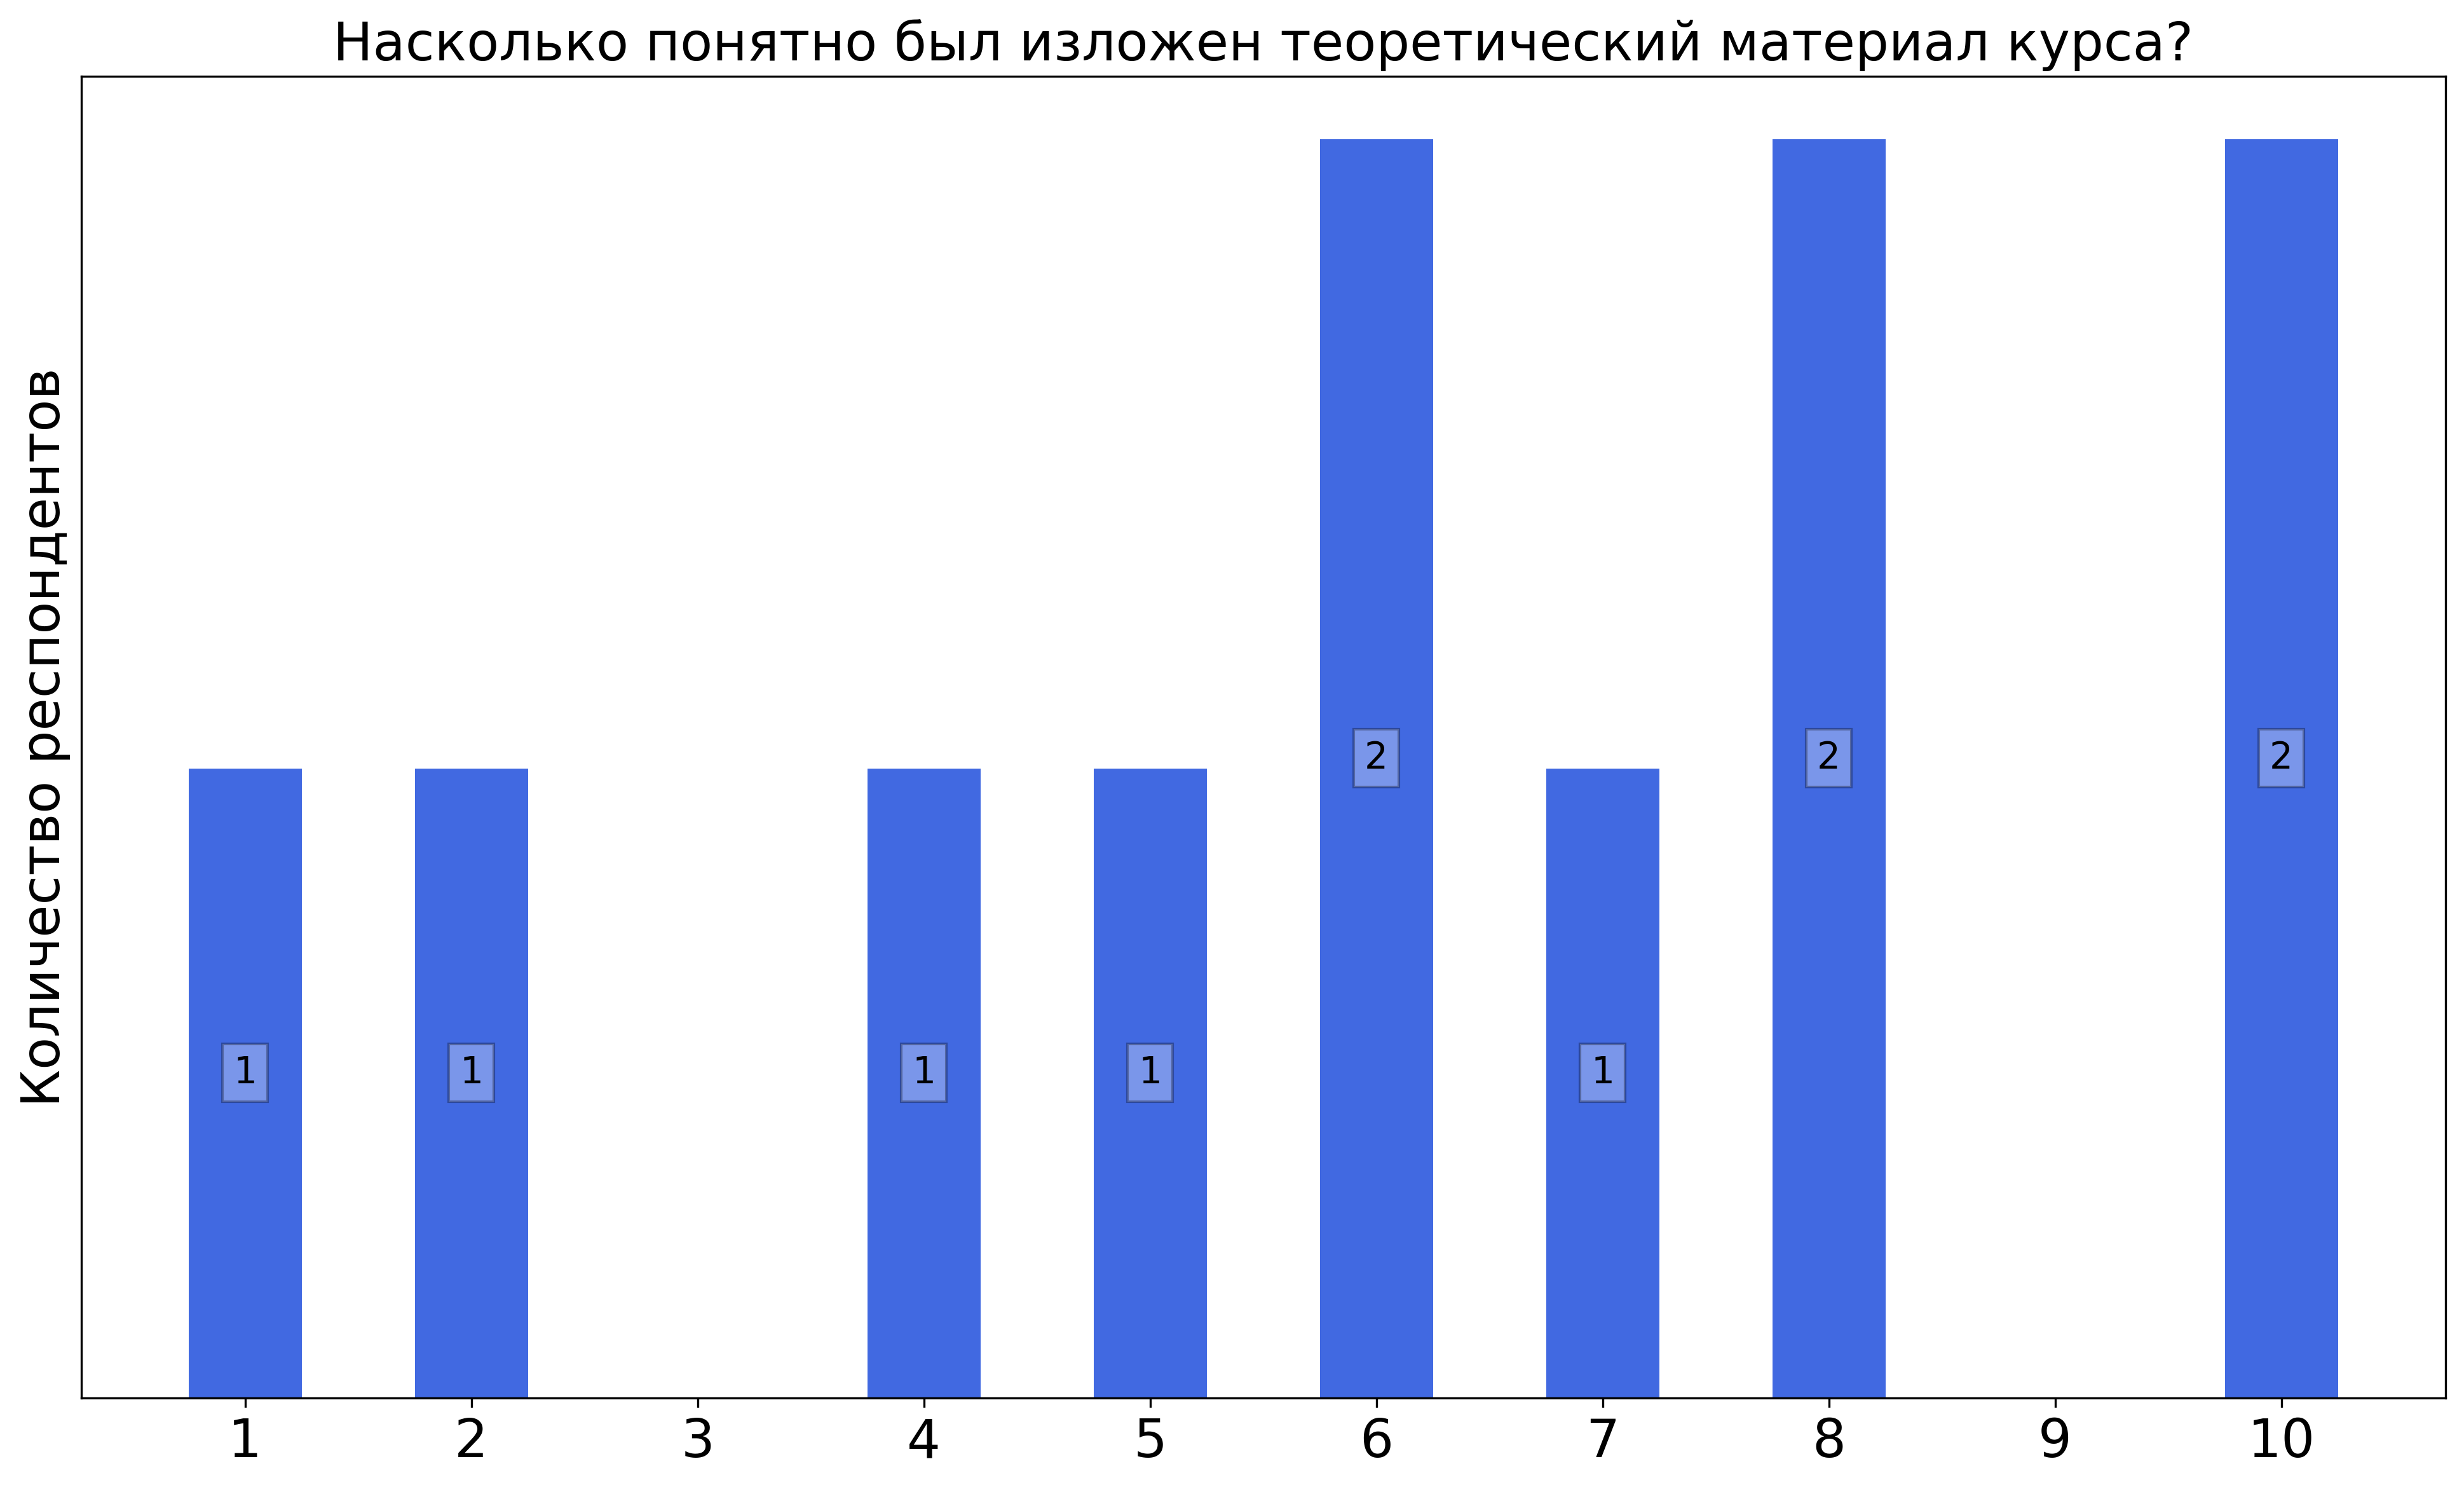
\includegraphics[width=\textwidth]{images/4 course/Защита информации/lecturer-marks-Колыбельников А.И.-2.png}
			\end{subfigure}	
			\begin{subfigure}[b]{0.45\textwidth}
				\centering
				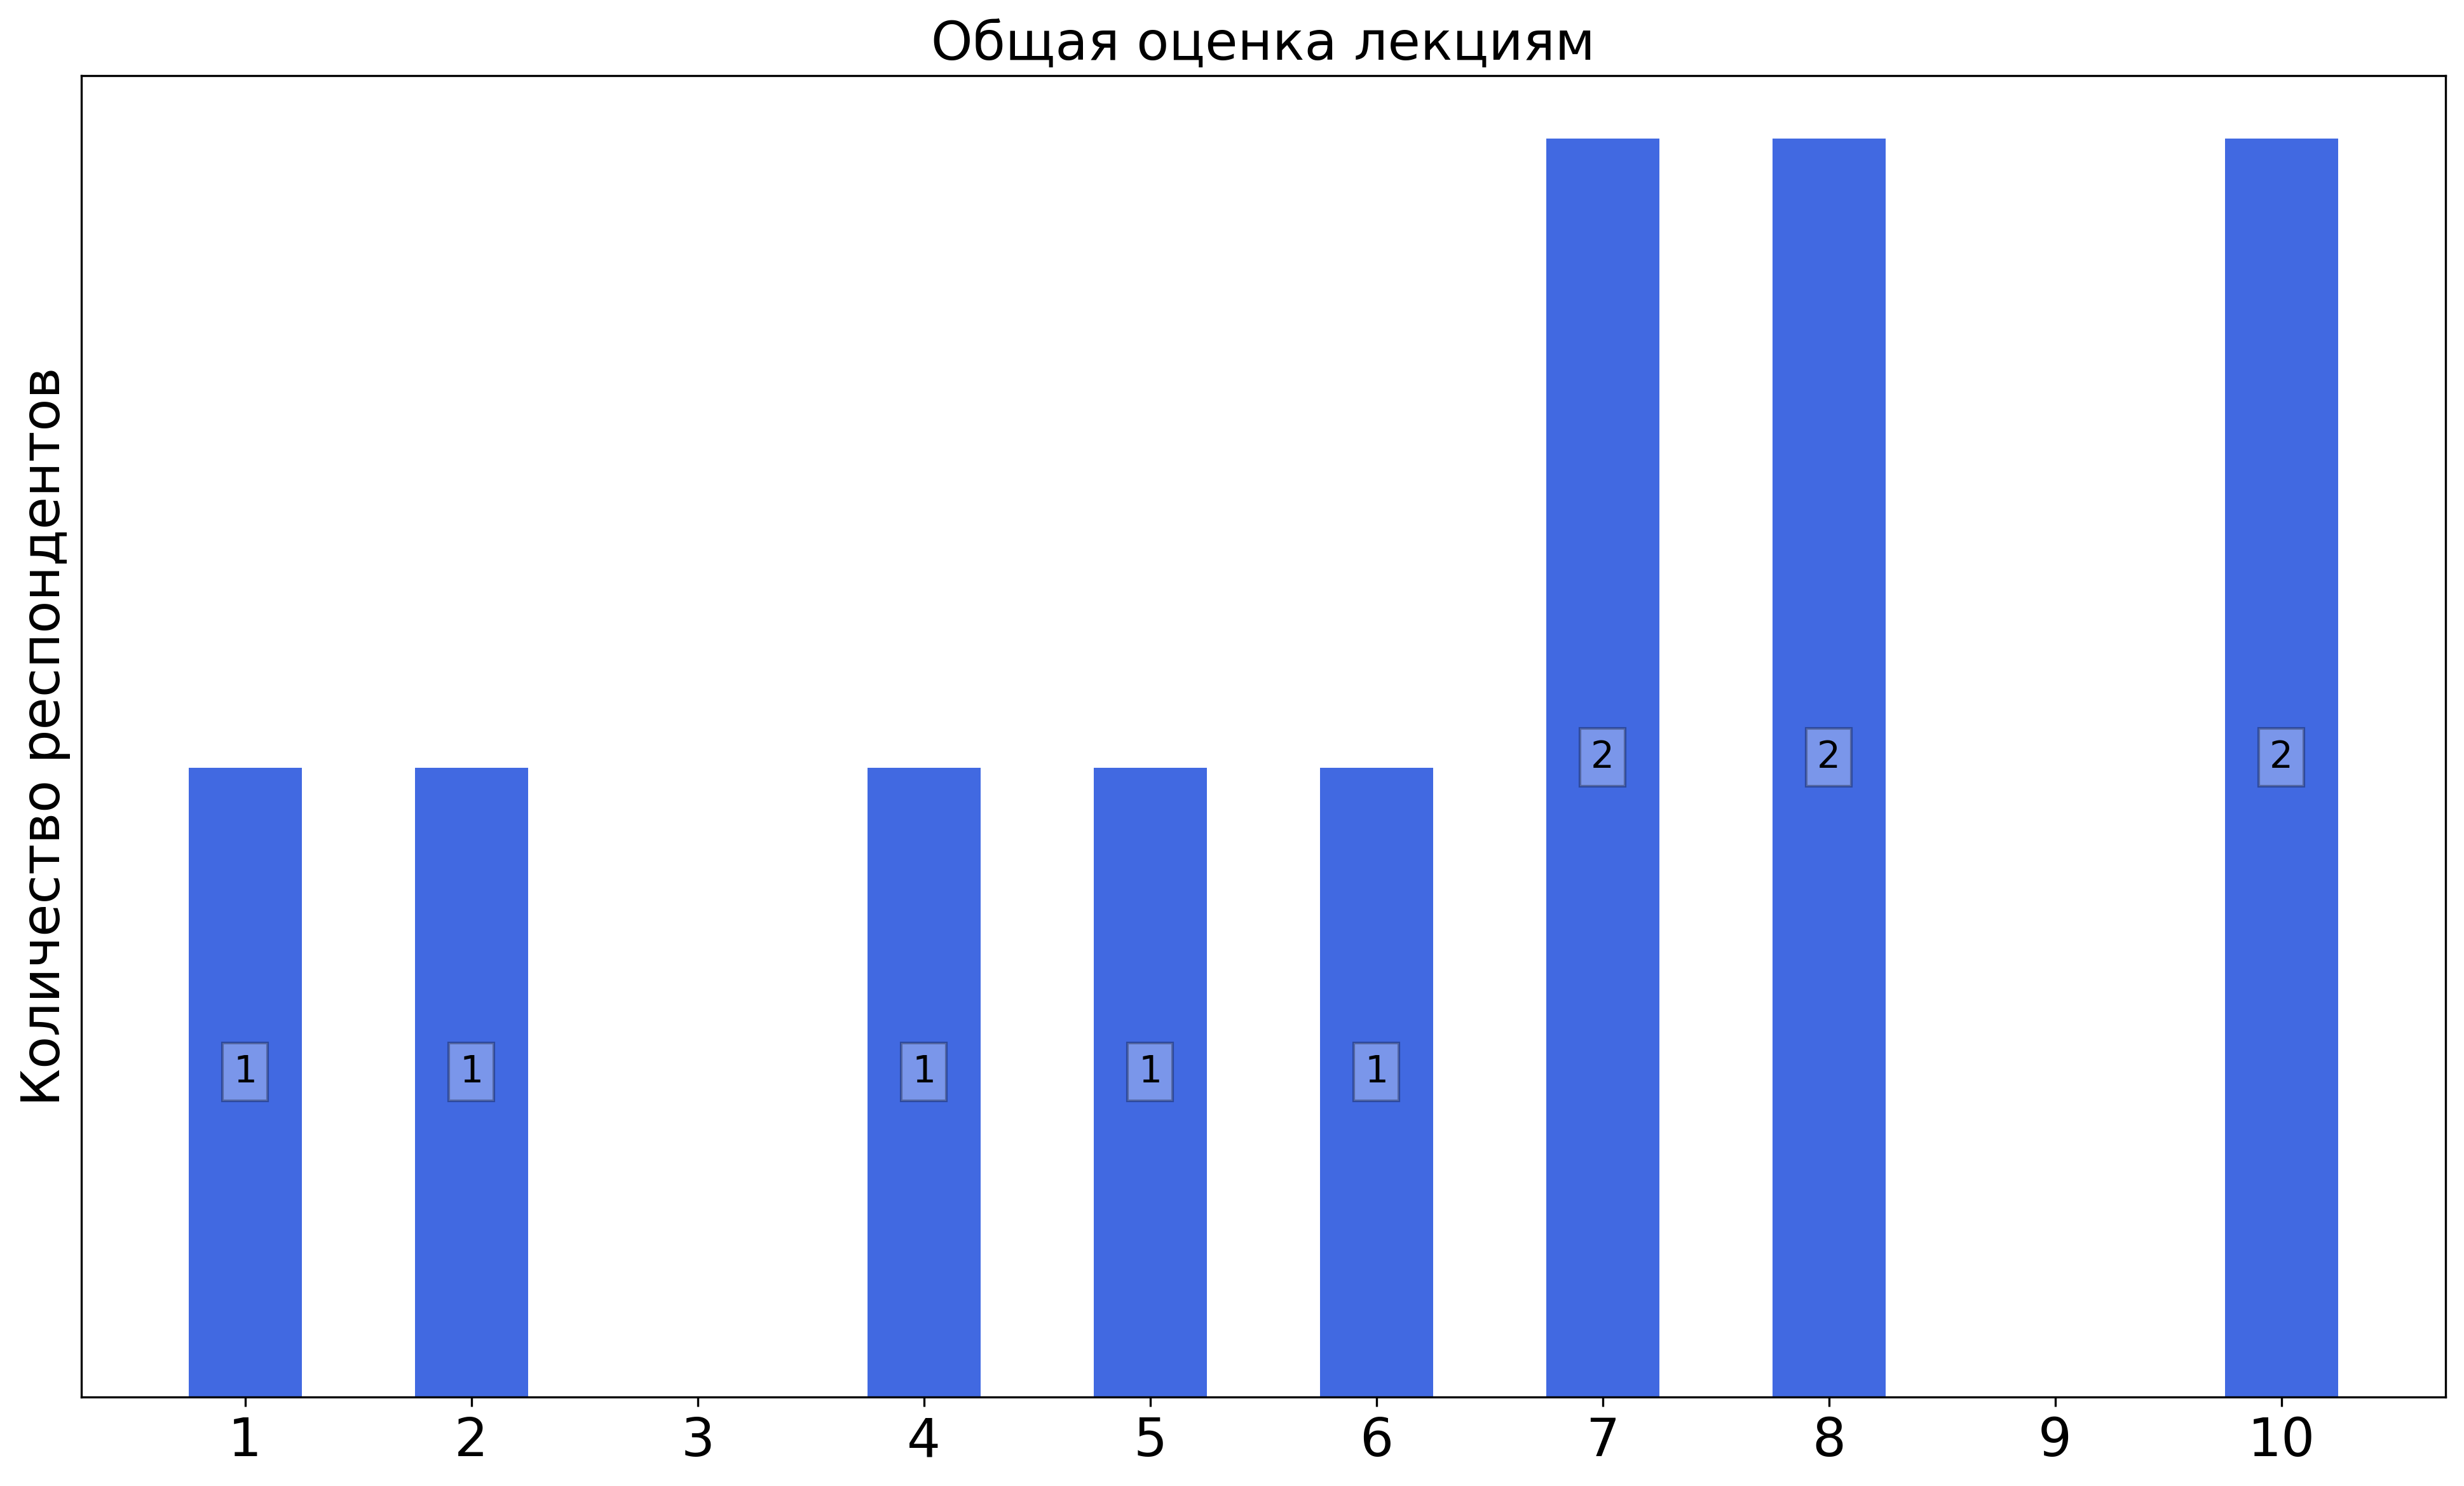
\includegraphics[width=\textwidth]{images/4 course/Защита информации/lecturer-marks-Колыбельников А.И.-3.png}
			\end{subfigure}
			\caption{Оценки респондентов о качестве преподавания лекций по курсу <<Защита информации>>}
		\end{figure}

		\textbf{Комментарии студентов о лекциях\protect\footnote{сохранены оригинальные орфография и пунктуация}} 
            \begin{commentbox} 
                На первых лекциях мне показалось что очень крутой курс и что наконец что то современное и востребованное но потом я немного разочаровалась и перестала ходить, наш семинарист рассказывал гораздо быстрее и понятнее суть алгоритмов и все нужное я могла найти в книжке, которая связана с курсом. 
                Меня также не понравилась идея, что студенты ради автомата за курс как будто должны публиковаться где то в статьях. Мне кажется если человек хочет написать и опубликовать какую то статью то и так это сделает. И в начале курса было не понятно насколько реально для автомата необходима была публикация статьи. Эссе мне тоже не понравилось как задание, а вот проект наоборот считаю интересным заданием. Необходимость сделать что то руками самим в командах увеличило интерес к предмету, а для эссе надо было просто по сути покопаться в интернете и сгенерить какую то сумму из того что уже есть 
            \end{commentbox} 

            \begin{commentbox} 
                Сходил на 1 лекцию, не могу что-то сказать конкретно. К 2й лекции (на которой был, лектор был подготовлен плохо)

                На защите рефератов (внутренней конференции) лектор показался мне знающим человеком 
            \end{commentbox}   
    
    
    \subsubsection{Отзыв студентов о семинарах. Семинарист: Аршанский А.Р.}
		\begin{figure}[H]
			\centering
			\begin{subfigure}[b]{0.45\textwidth}
				\centering
				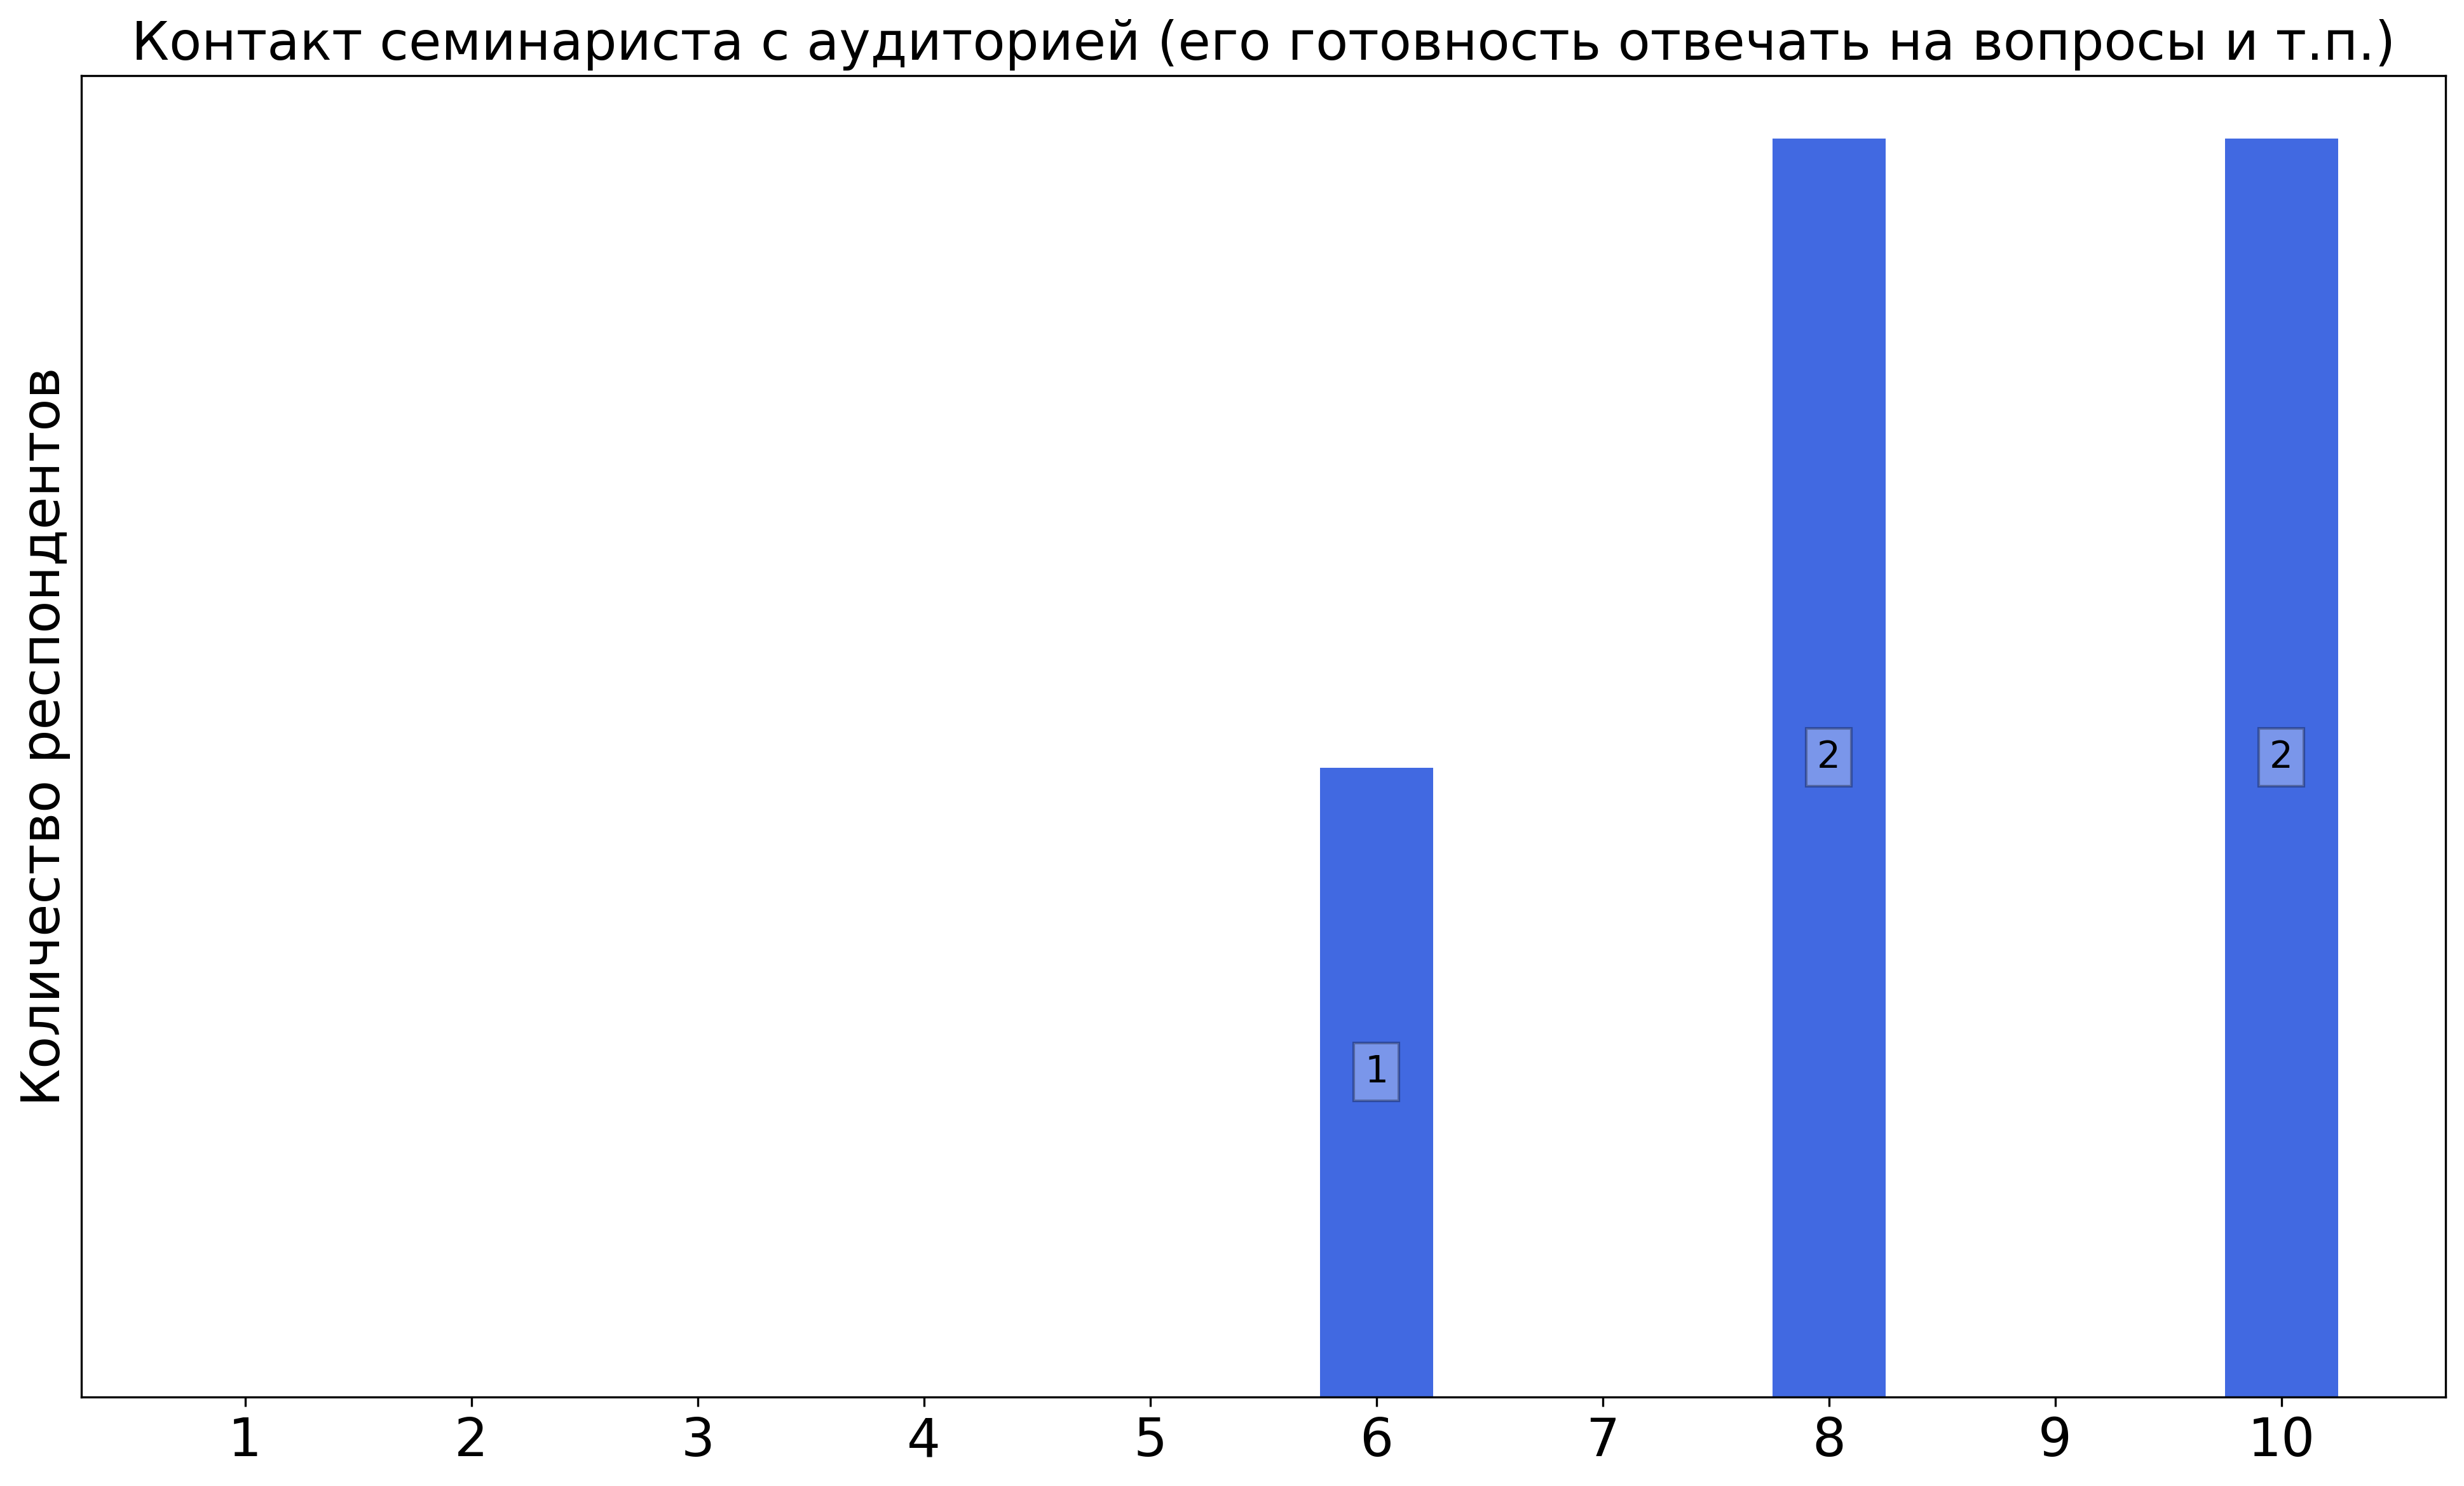
\includegraphics[width=\textwidth]{images/4 course/Защита информации/seminarists-marks-Аршанский А.Р.-0.png}
			\end{subfigure}
			\begin{subfigure}[b]{0.45\textwidth}
				\centering
				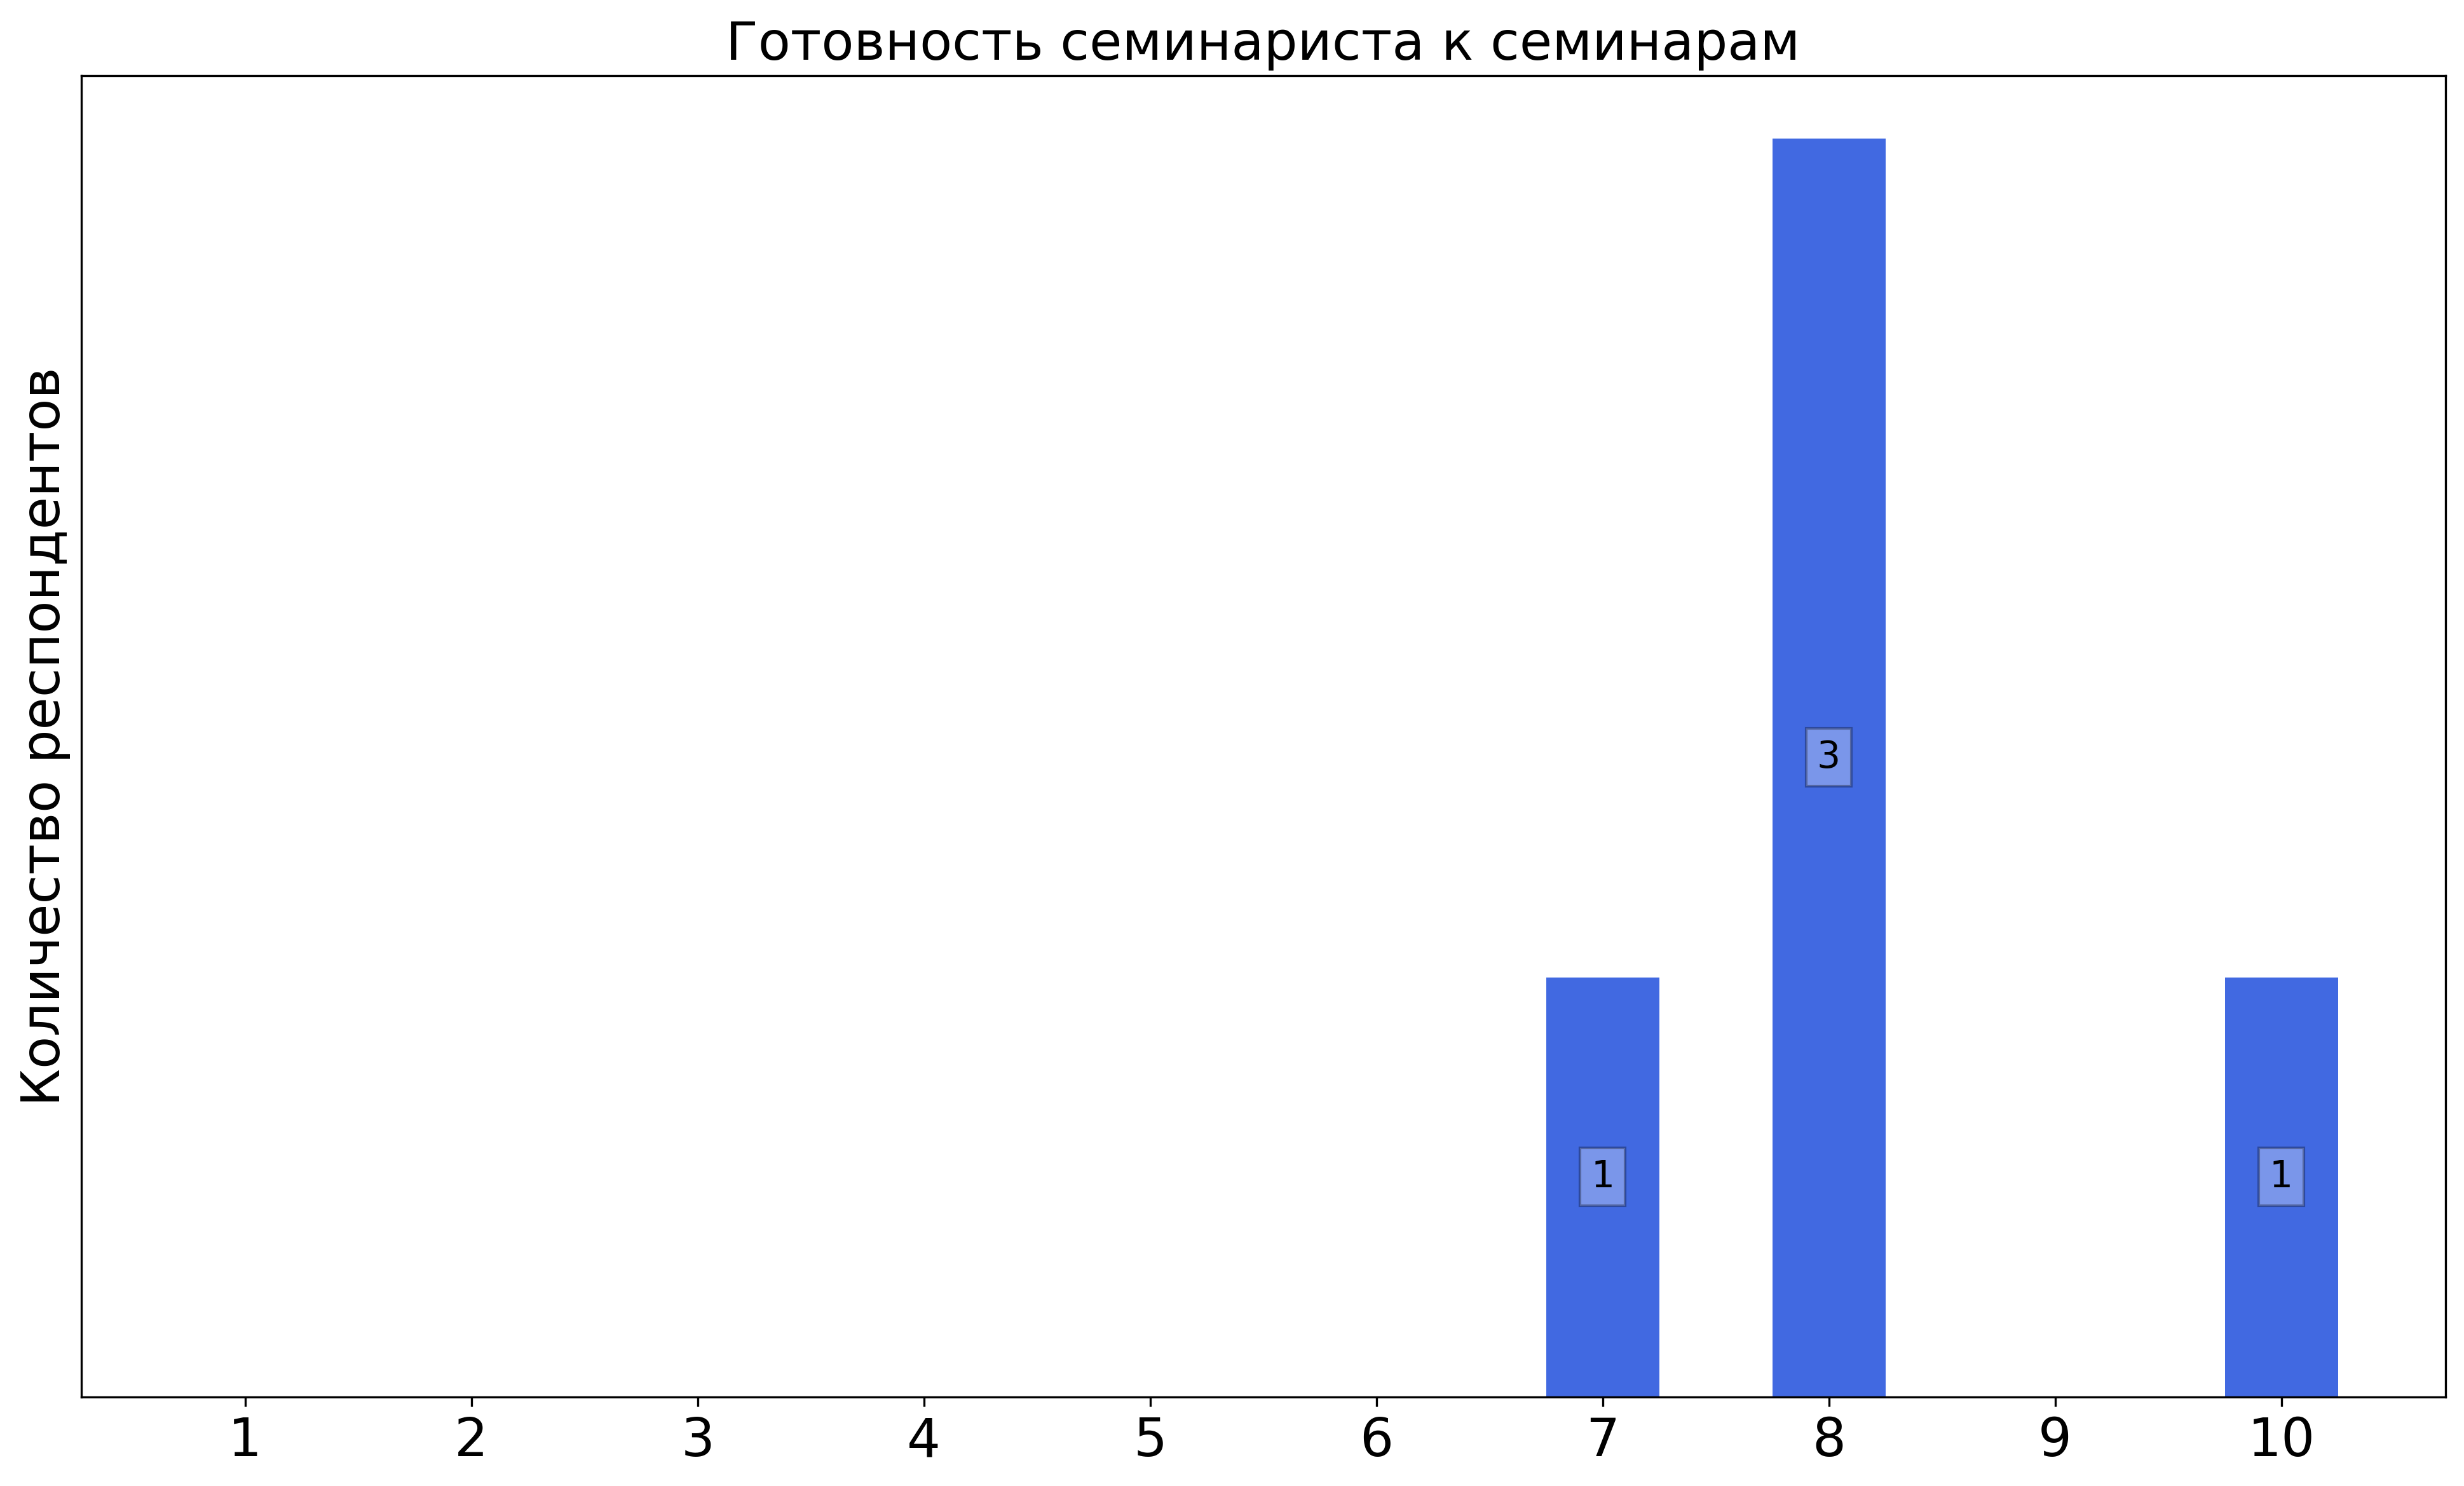
\includegraphics[width=\textwidth]{images/4 course/Защита информации/seminarists-marks-Аршанский А.Р.-1.png}
			\end{subfigure}
			\begin{subfigure}[b]{0.45\textwidth}
				\centering
				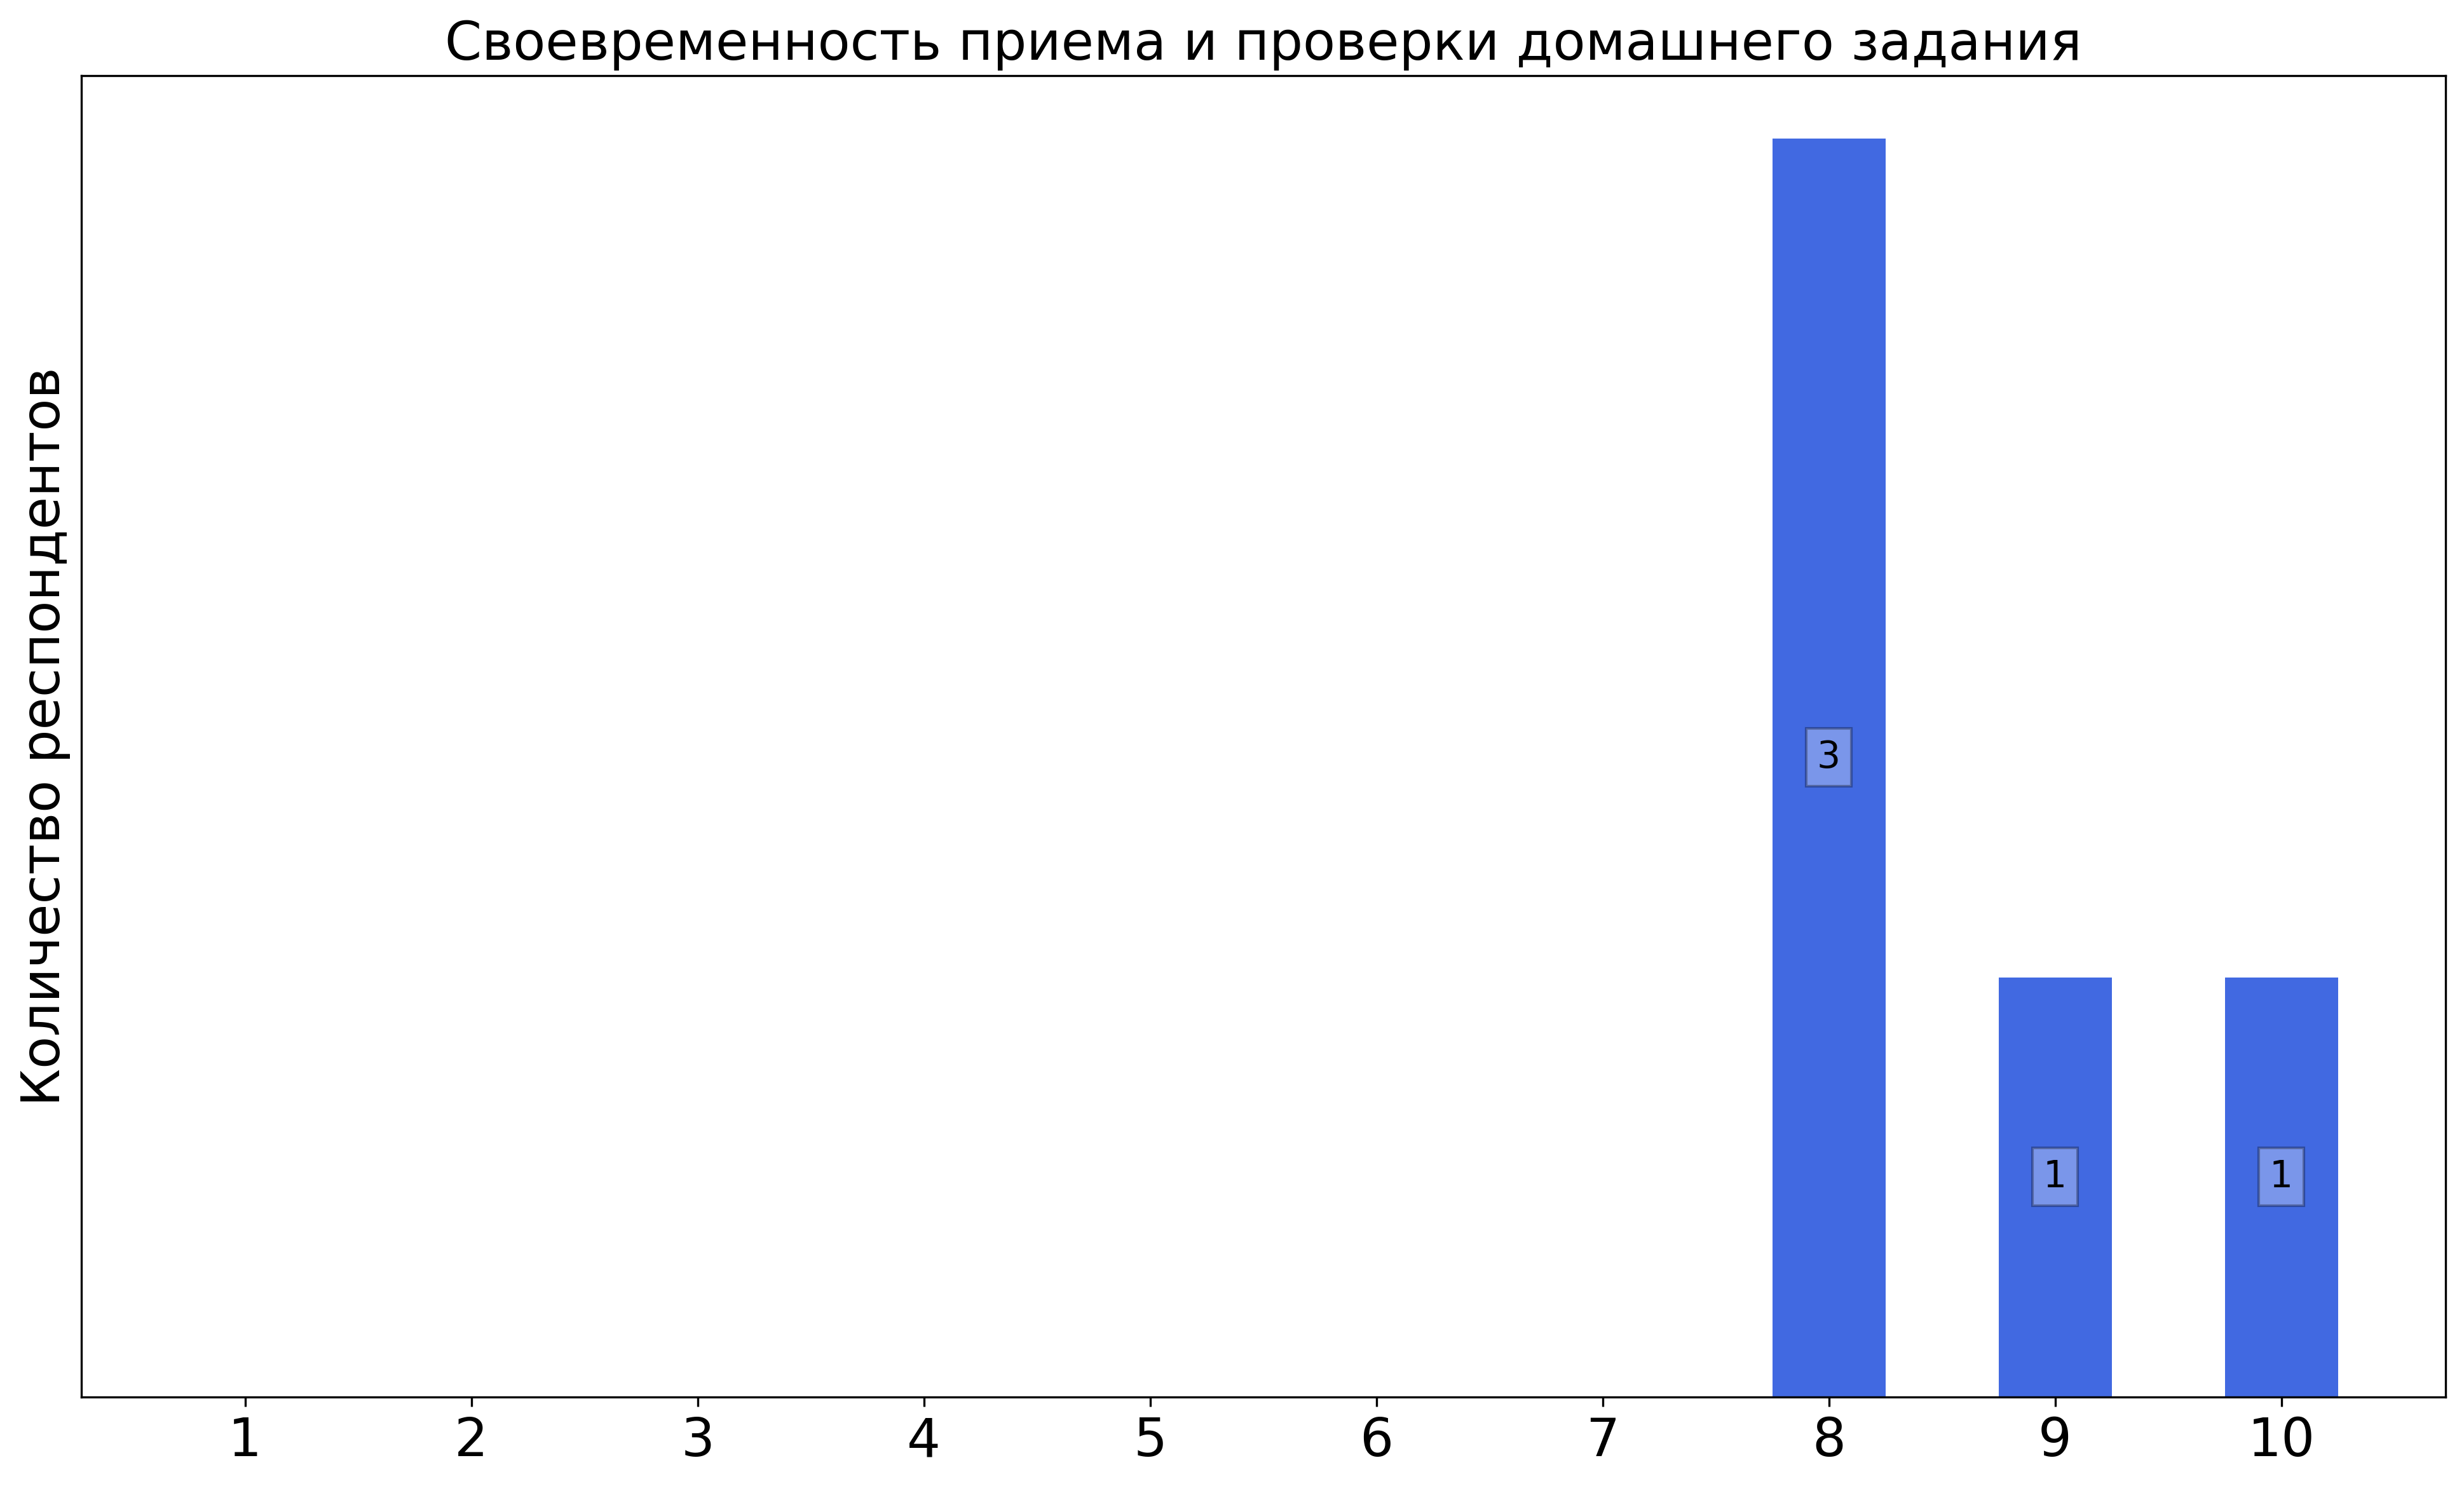
\includegraphics[width=\textwidth]{images/4 course/Защита информации/seminarists-marks-Аршанский А.Р.-2.png}
			\end{subfigure}
			\begin{subfigure}[b]{0.45\textwidth}
				\centering
				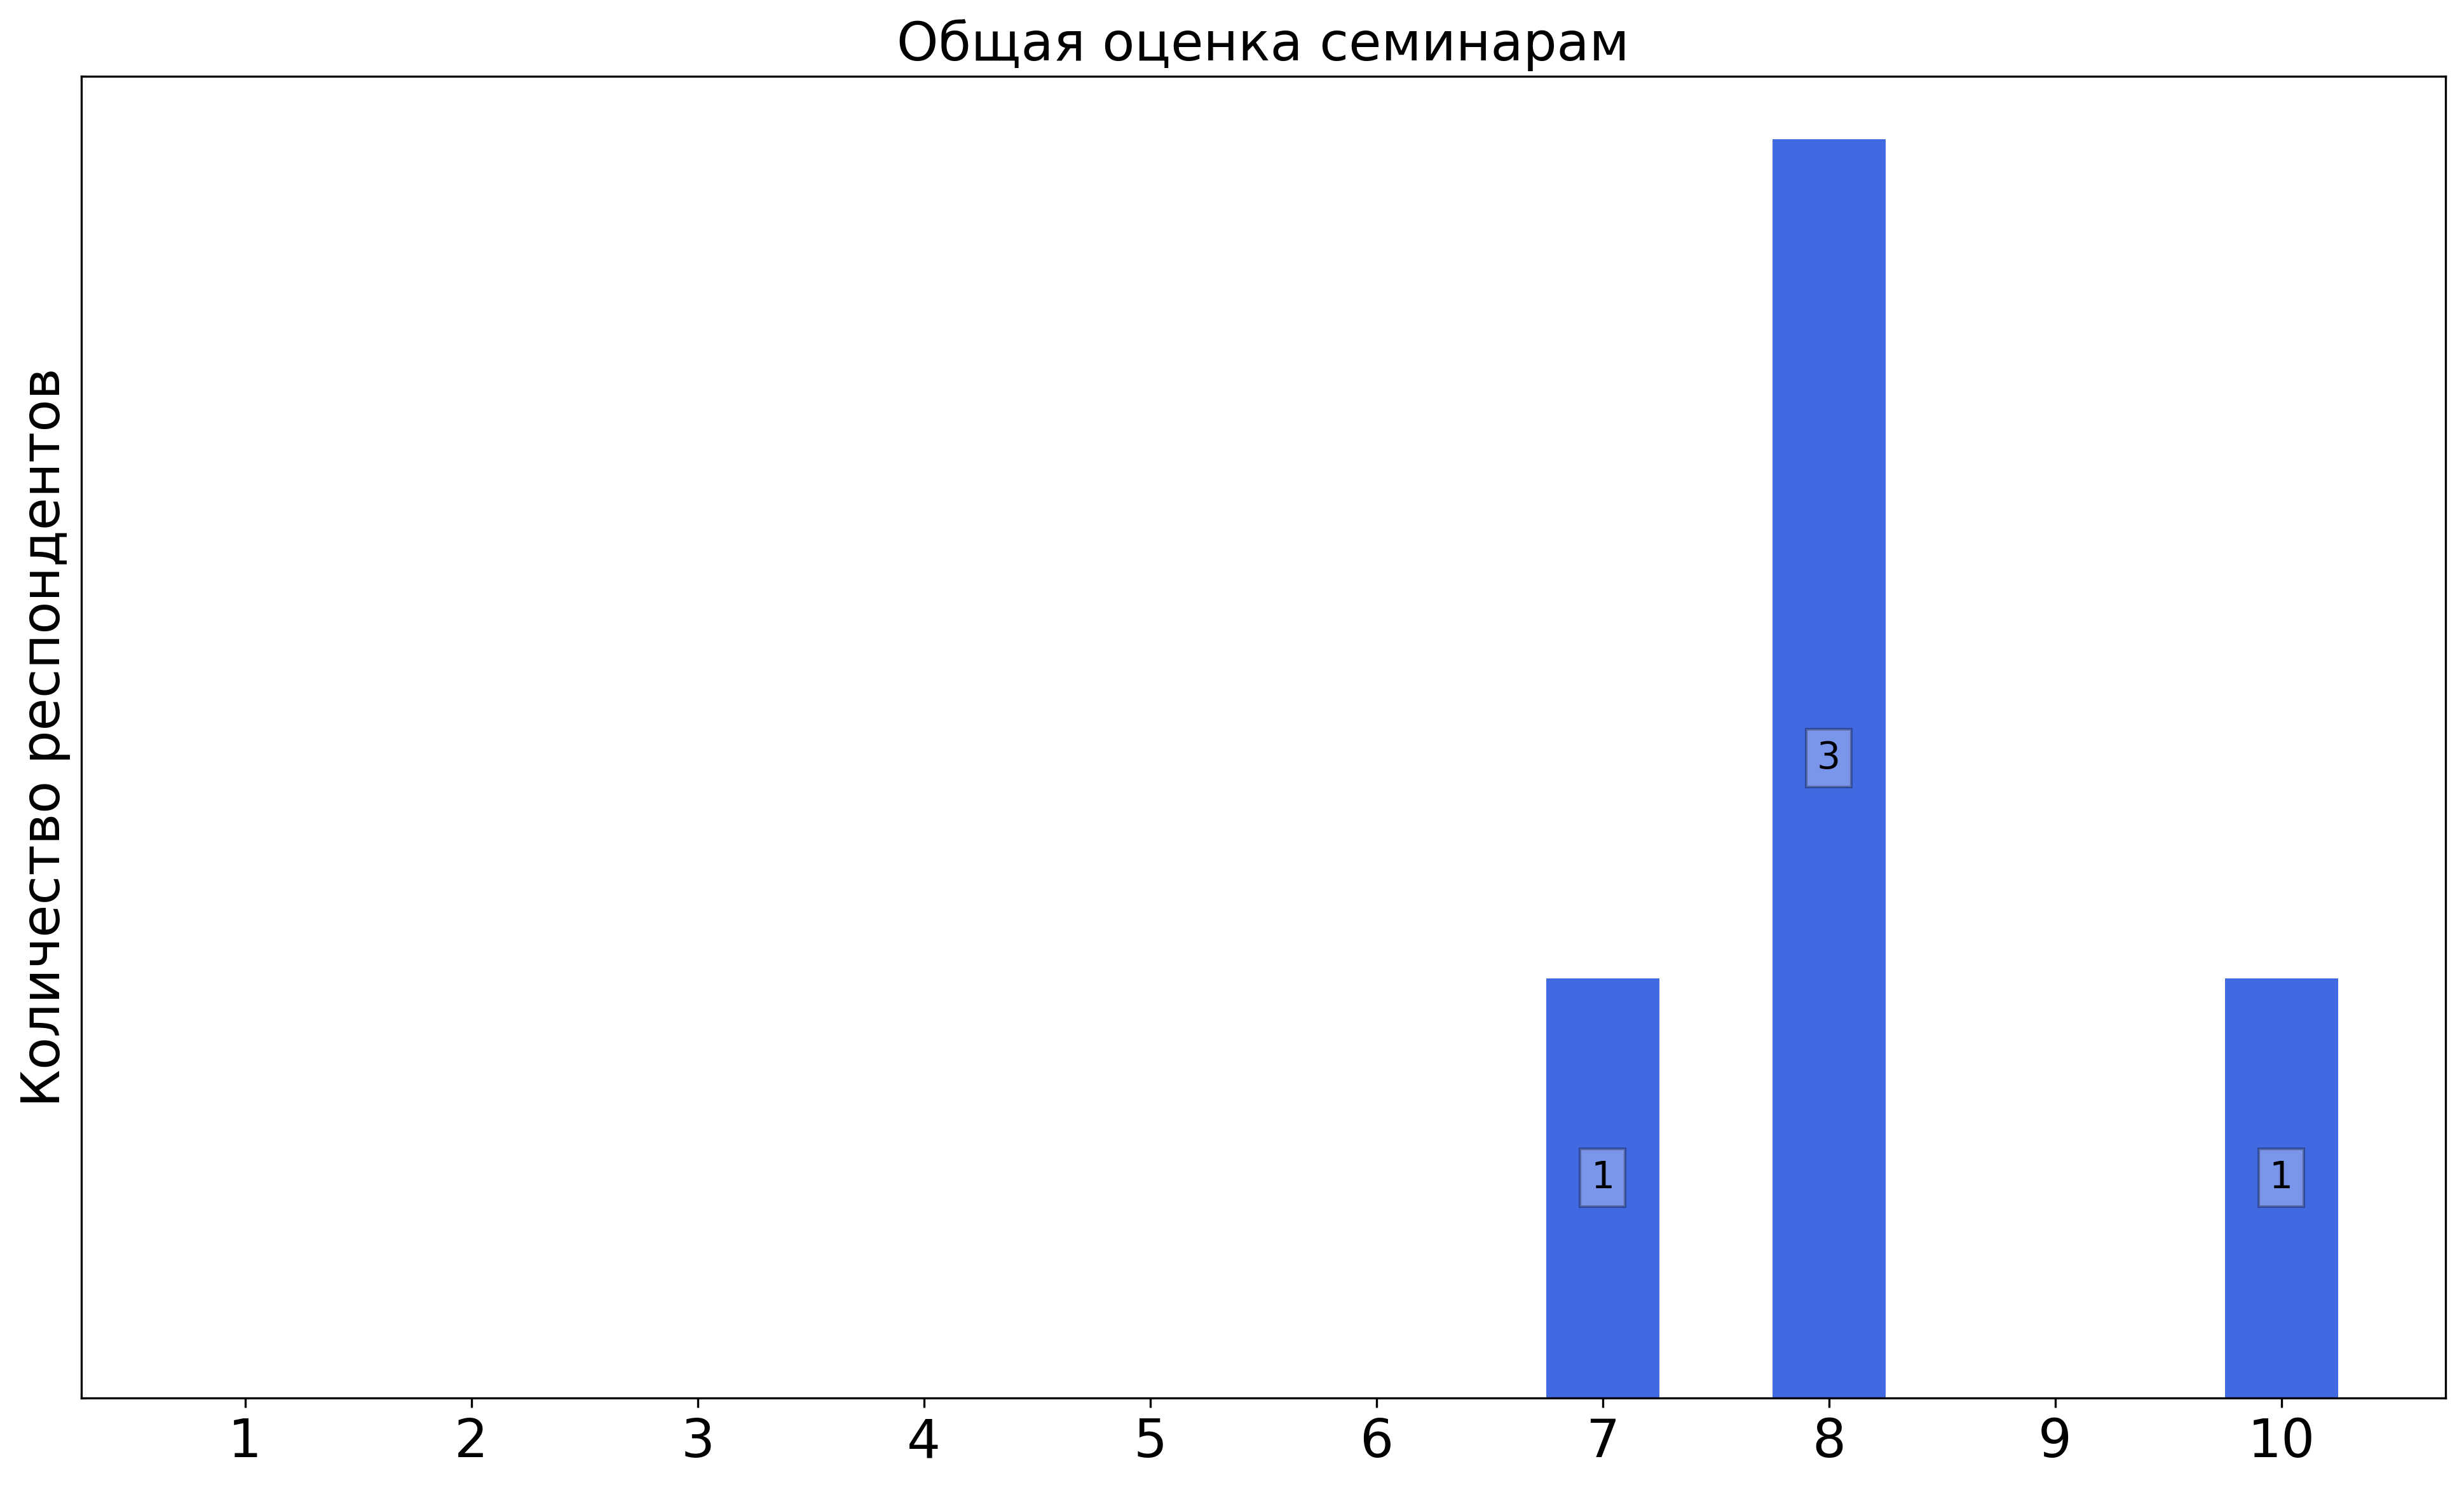
\includegraphics[width=\textwidth]{images/4 course/Защита информации/seminarists-marks-Аршанский А.Р.-3.png}
			\end{subfigure}	
			\caption{Оценки респондентов о качестве преподавания семинаров}
		\end{figure}

		\textbf{Комментарии студентов о семинаристе\protect\footnote{сохранены оригинальные орфография и пунктуация}}
            \begin{commentbox} 
                Отлично объяснял: быстро и по делу, свободная посещаемость, добрый и позитивный. Контрольные можно отаппелировать, эссе сдавалось в удобном формате, проекты хорошо принимал, все своевременно. Перевелась к нему, потому что до этого было у Семаки приходилось на парах к доске выходить и по моему для студентов 4 курса это бред. 
            \end{commentbox} 

              
    \subsubsection{Отзыв студентов о семинарах. Семинарист: Григорьев И.А.}
        \begin{figure}[H]
            \centering
            \begin{subfigure}[b]{0.45\textwidth}
                \centering
                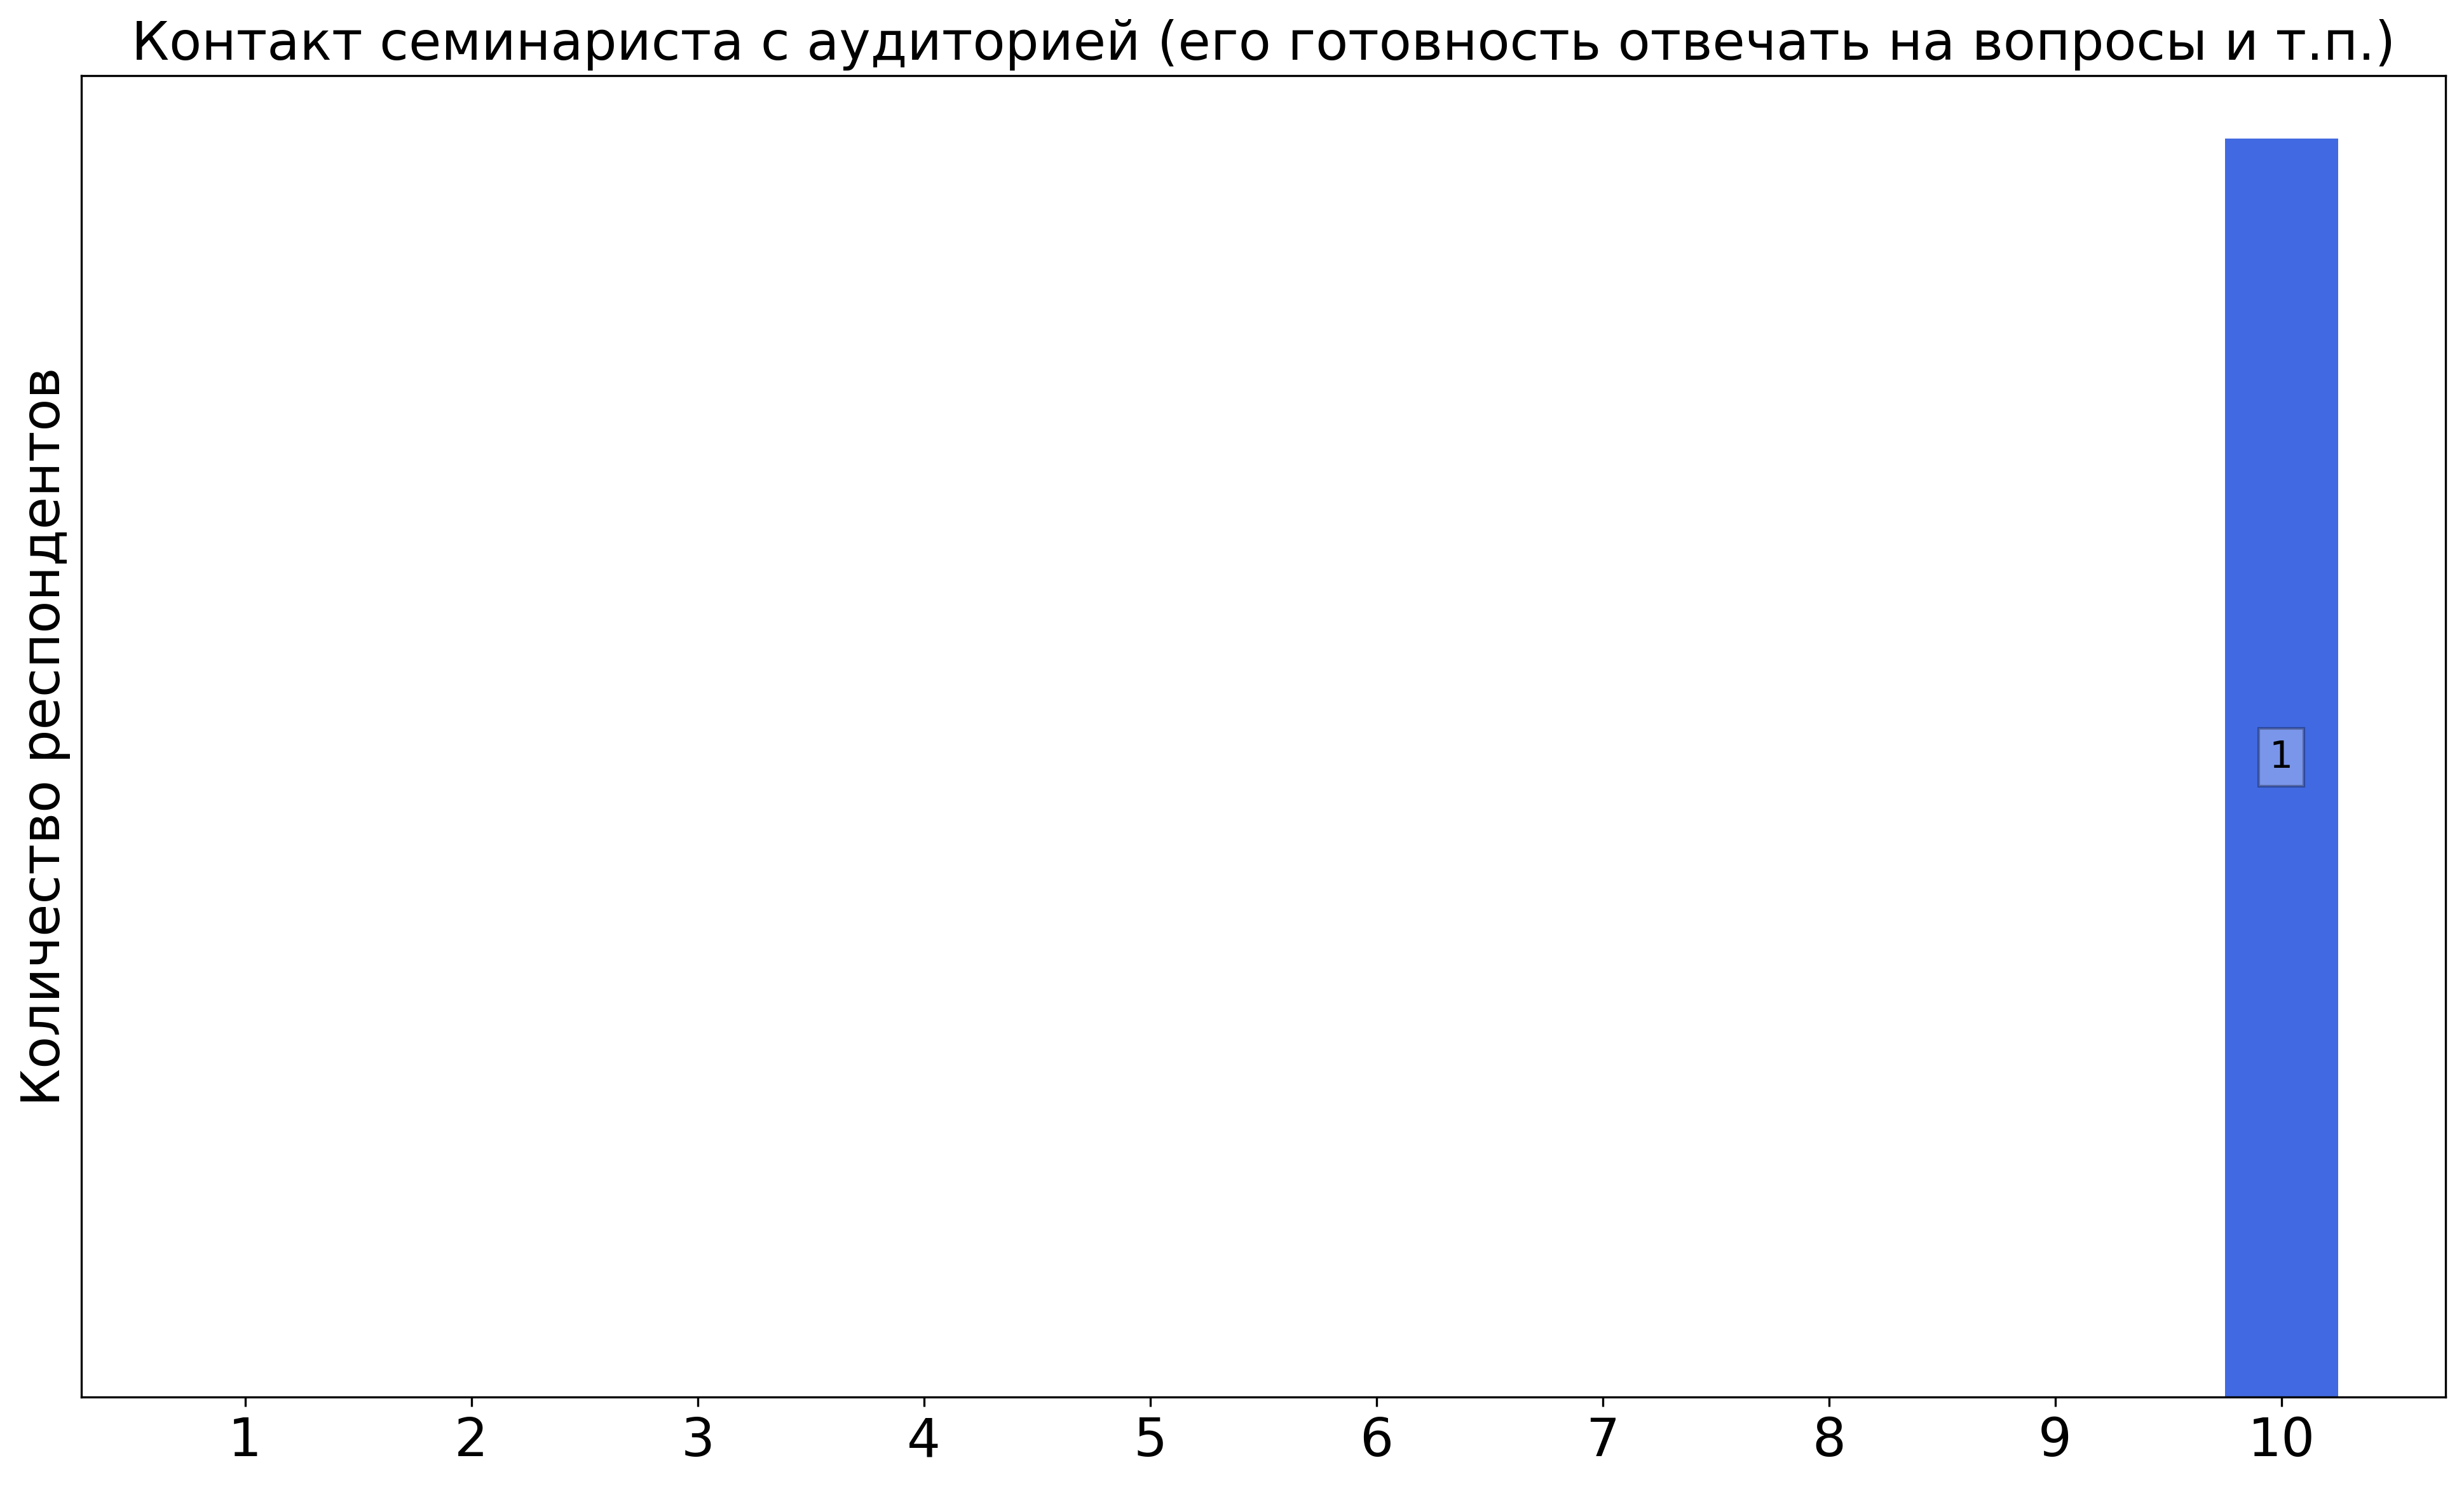
\includegraphics[width=\textwidth]{images/4 course/Защита информации/seminarists-marks-Григорьев И.А.-0.png}
            \end{subfigure}
            \begin{subfigure}[b]{0.45\textwidth}
                \centering
                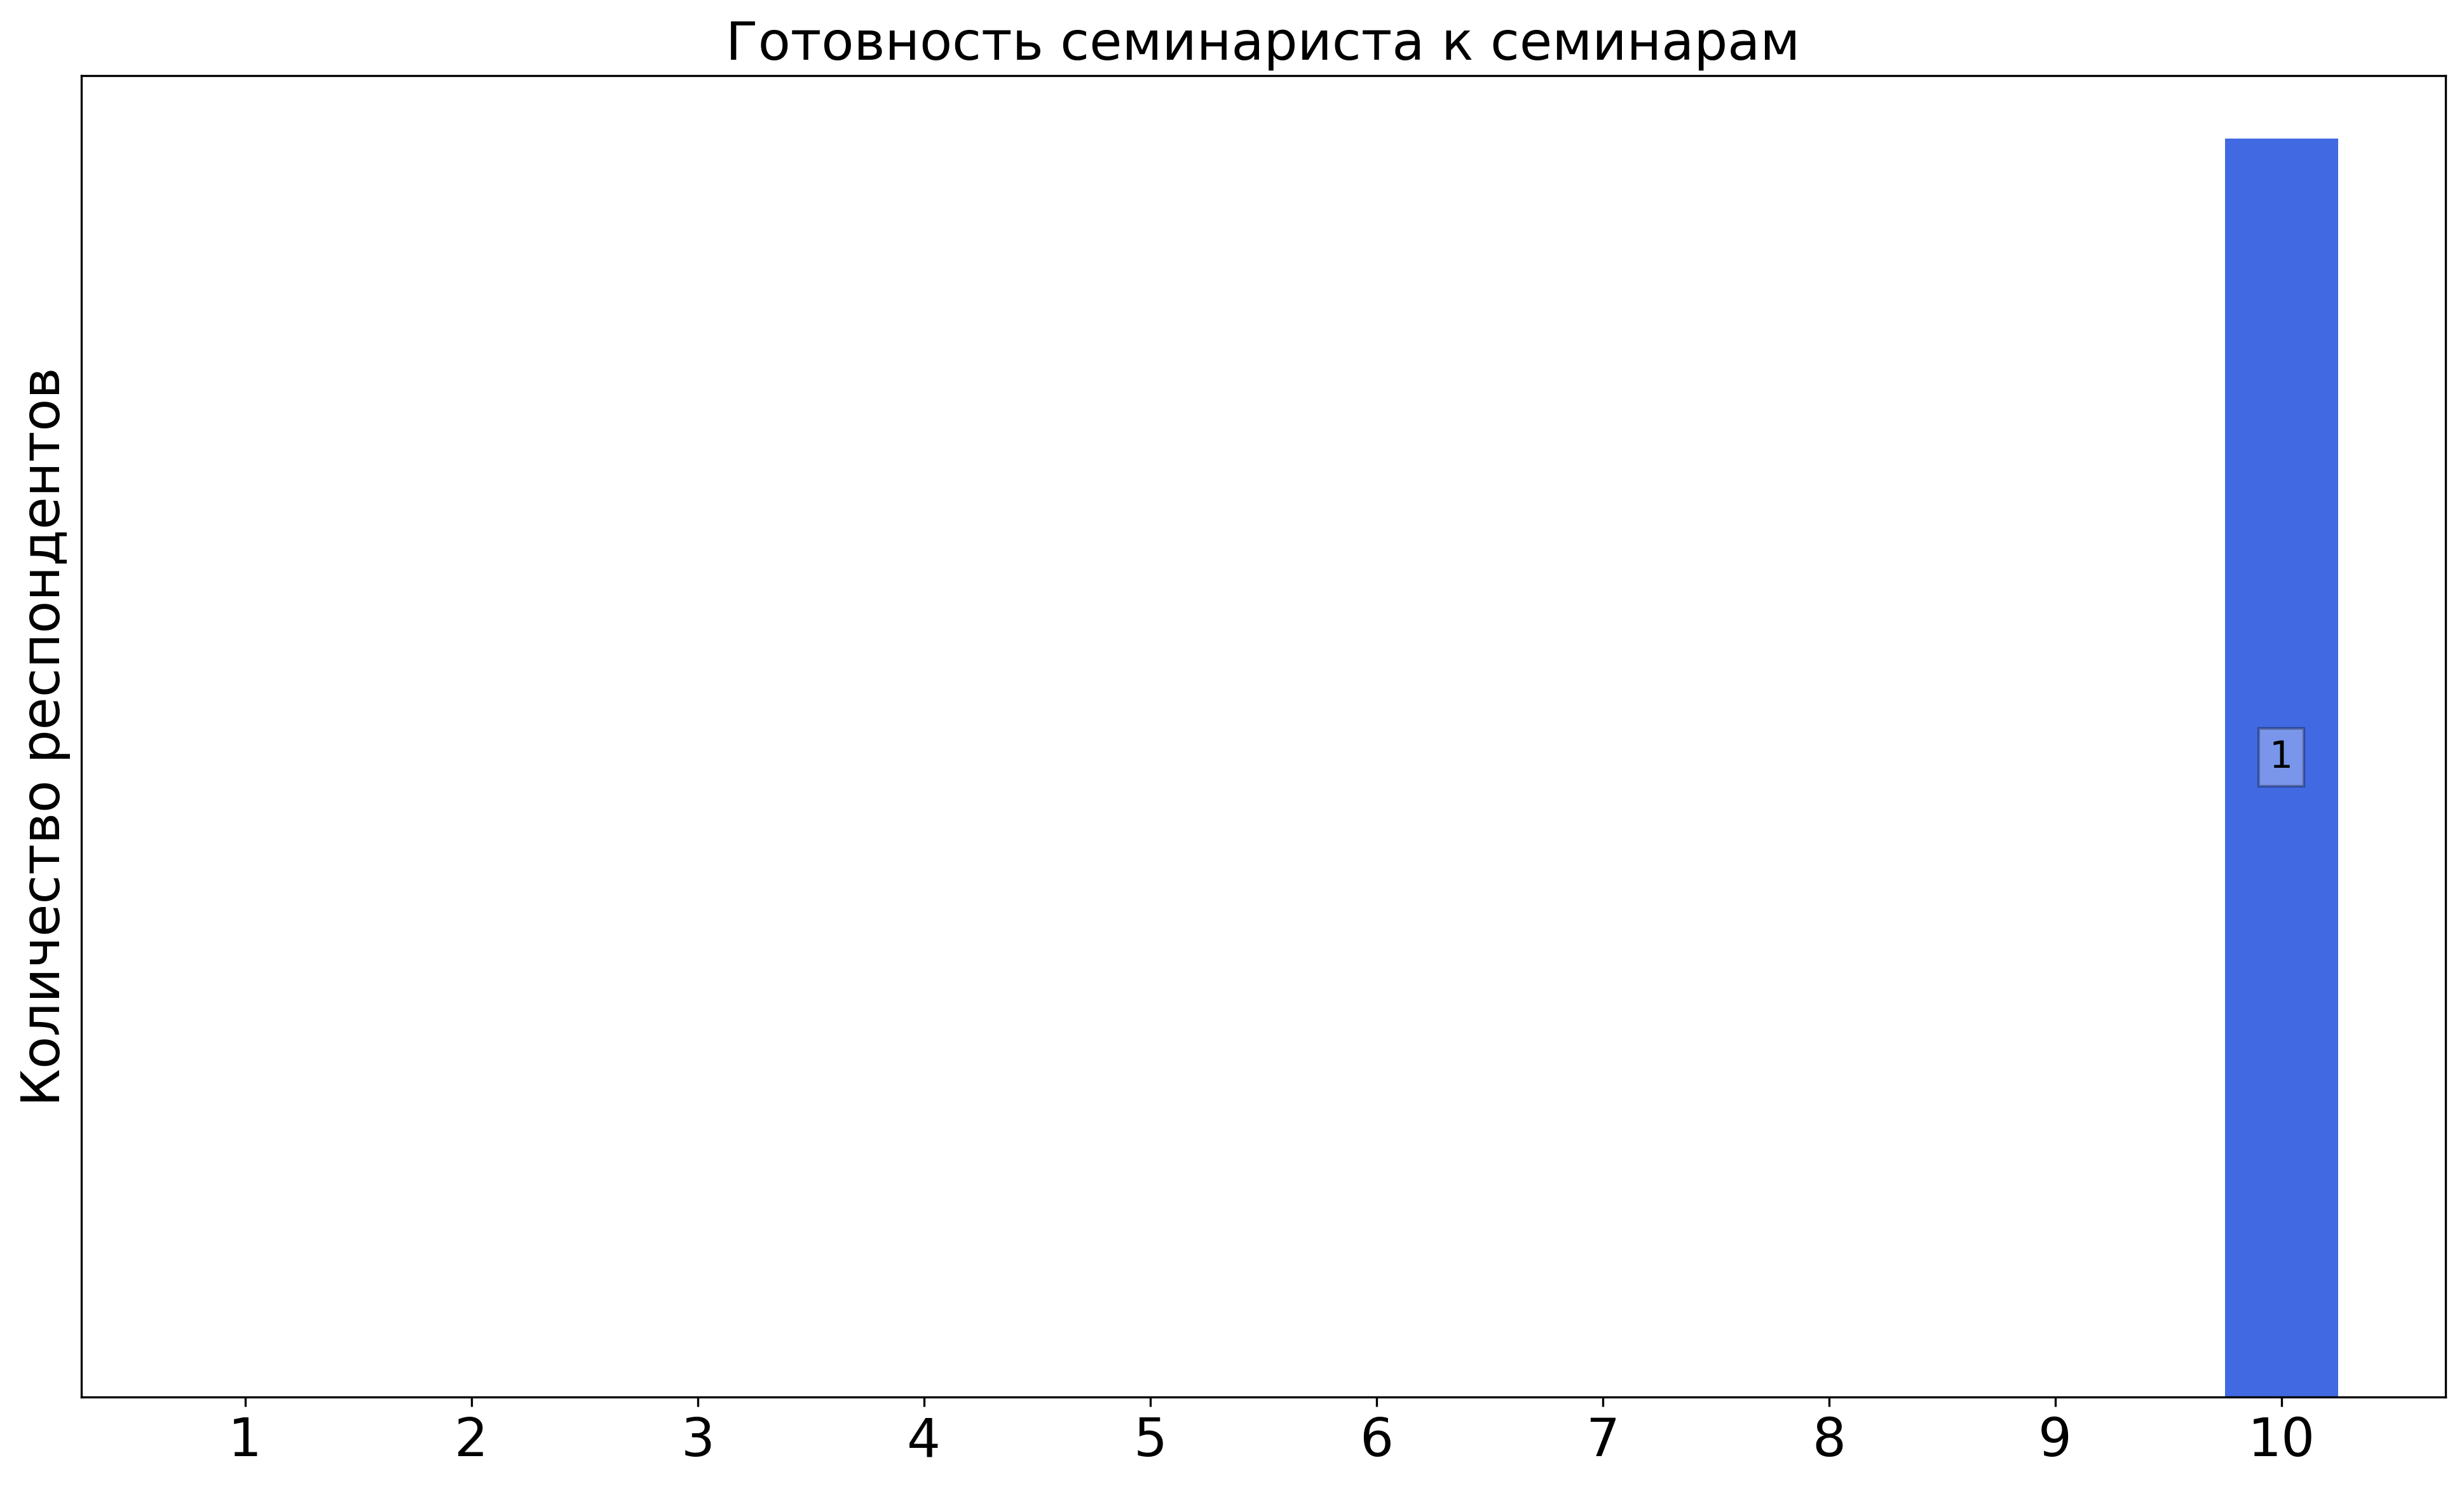
\includegraphics[width=\textwidth]{images/4 course/Защита информации/seminarists-marks-Григорьев И.А.-1.png}
            \end{subfigure}
            \begin{subfigure}[b]{0.45\textwidth}
                \centering
                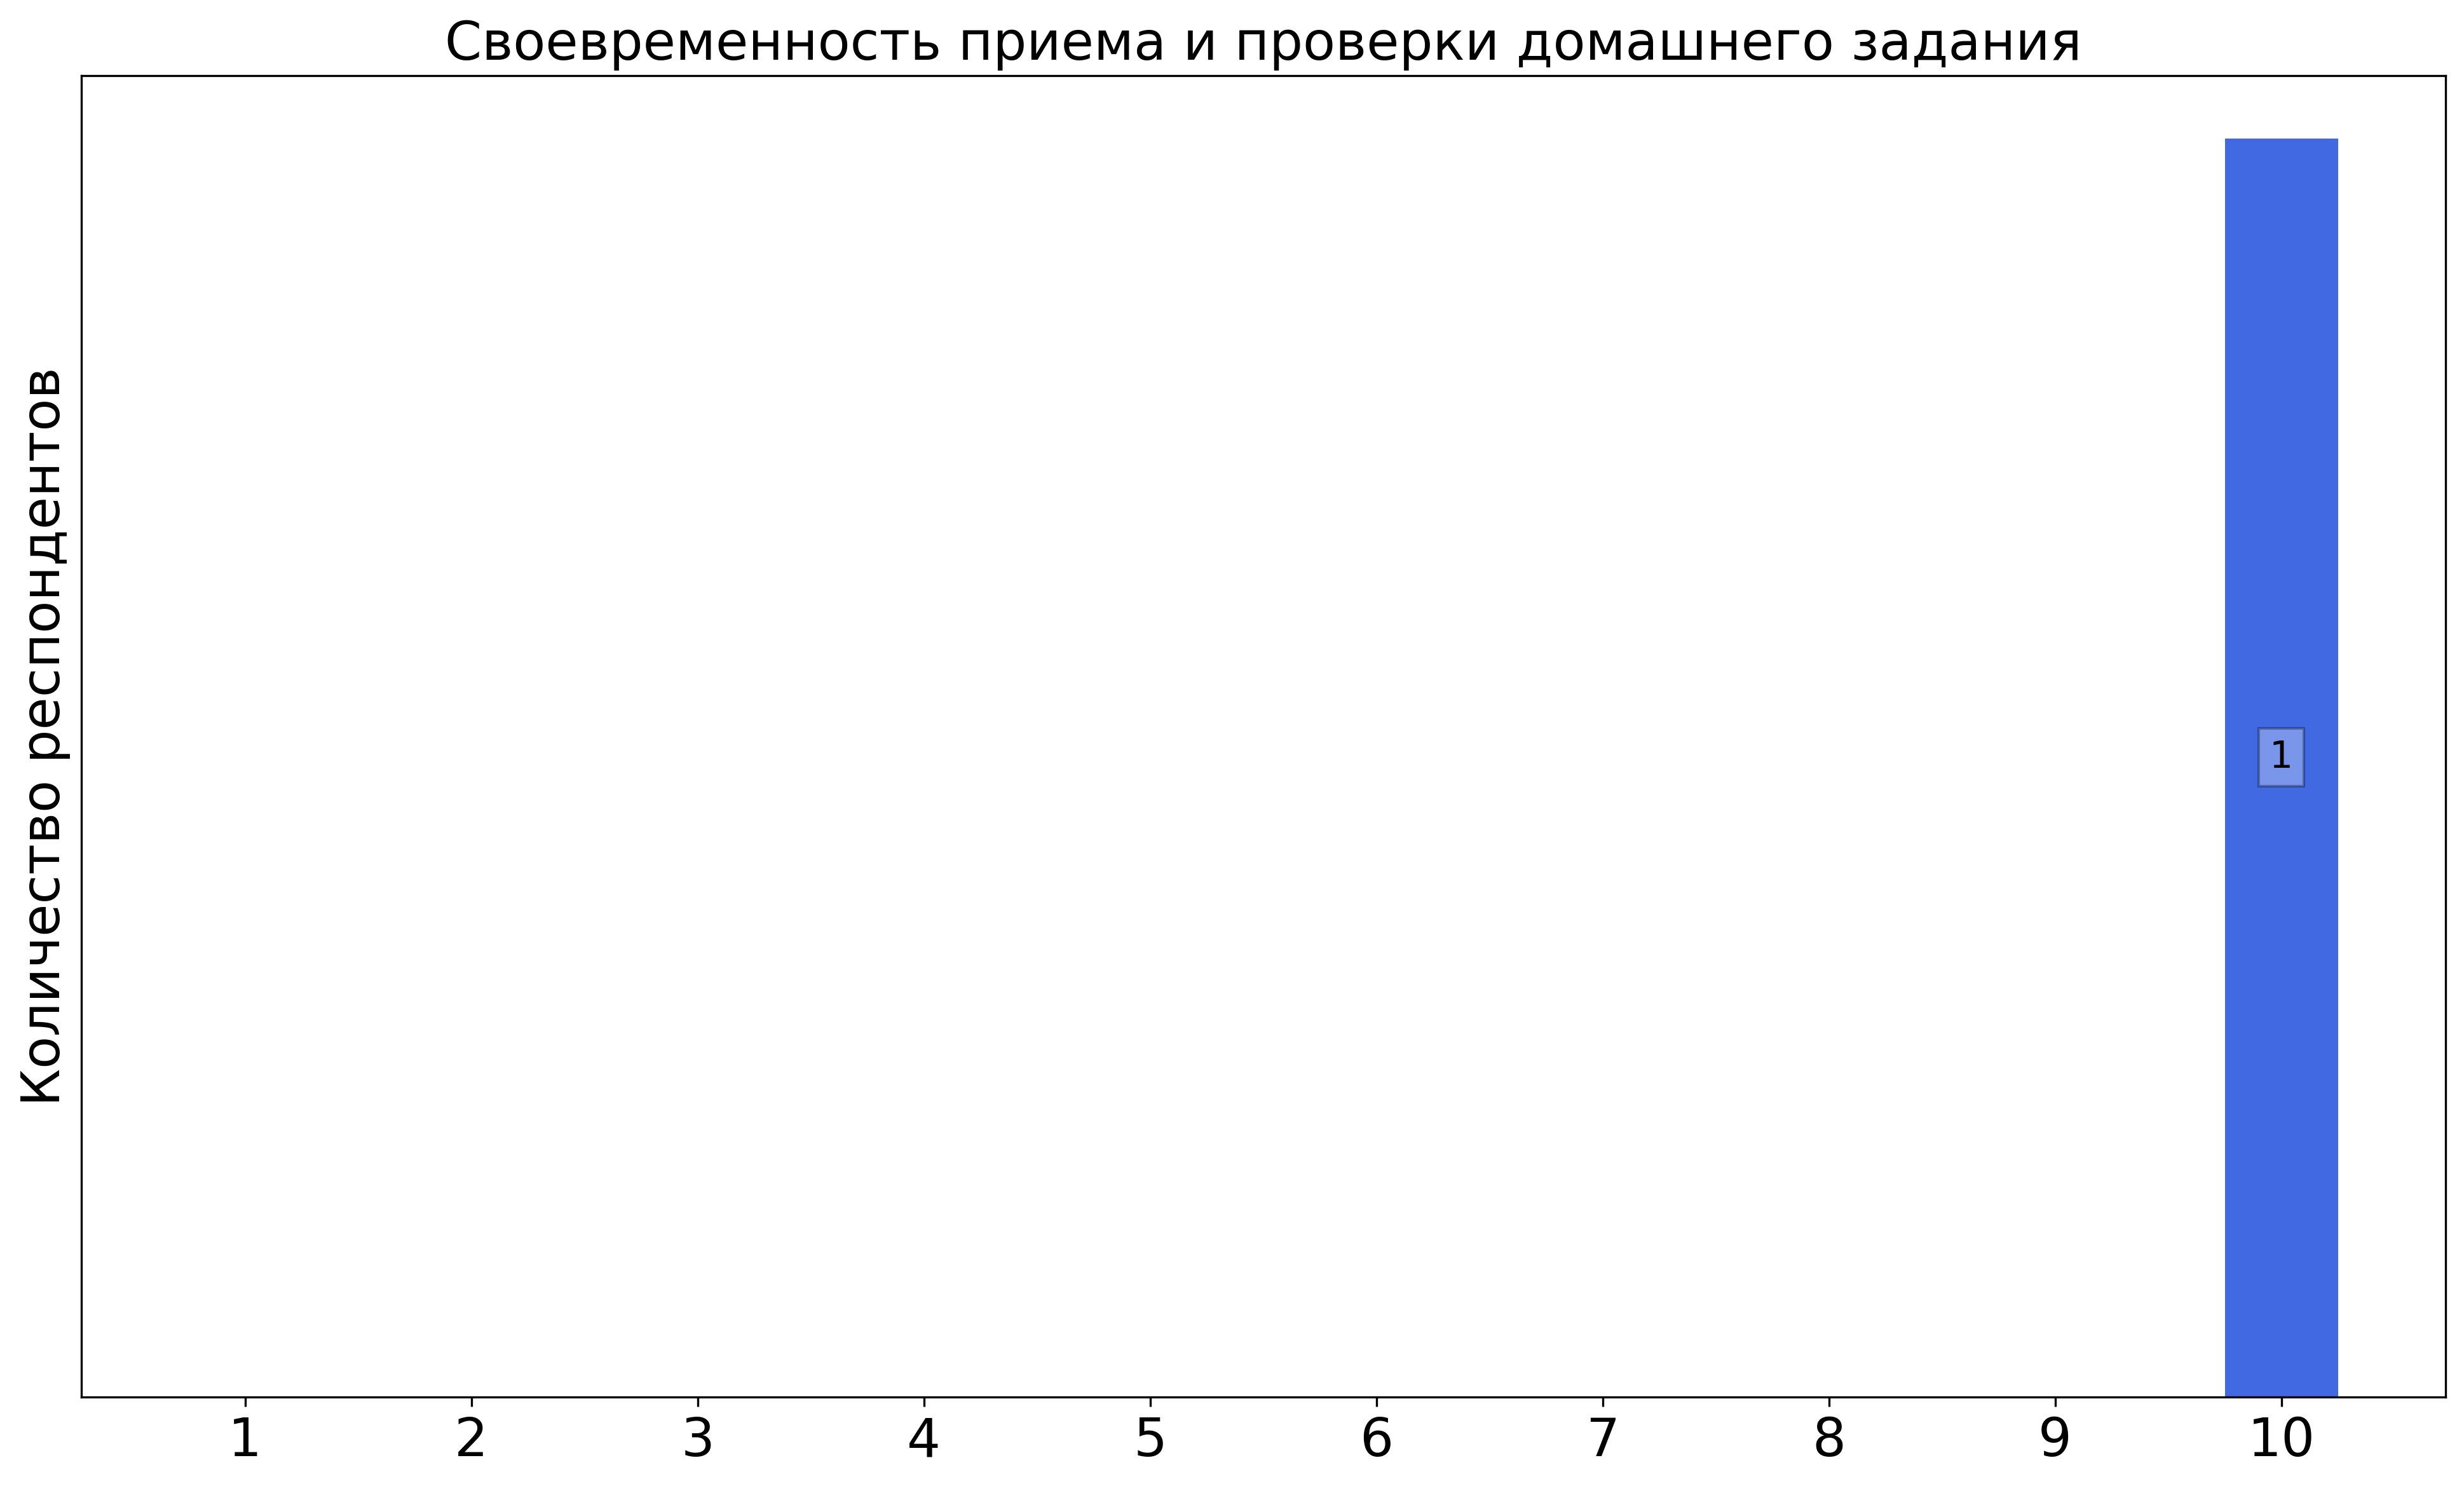
\includegraphics[width=\textwidth]{images/4 course/Защита информации/seminarists-marks-Григорьев И.А.-2.png}
            \end{subfigure}
            \begin{subfigure}[b]{0.45\textwidth}
                \centering
                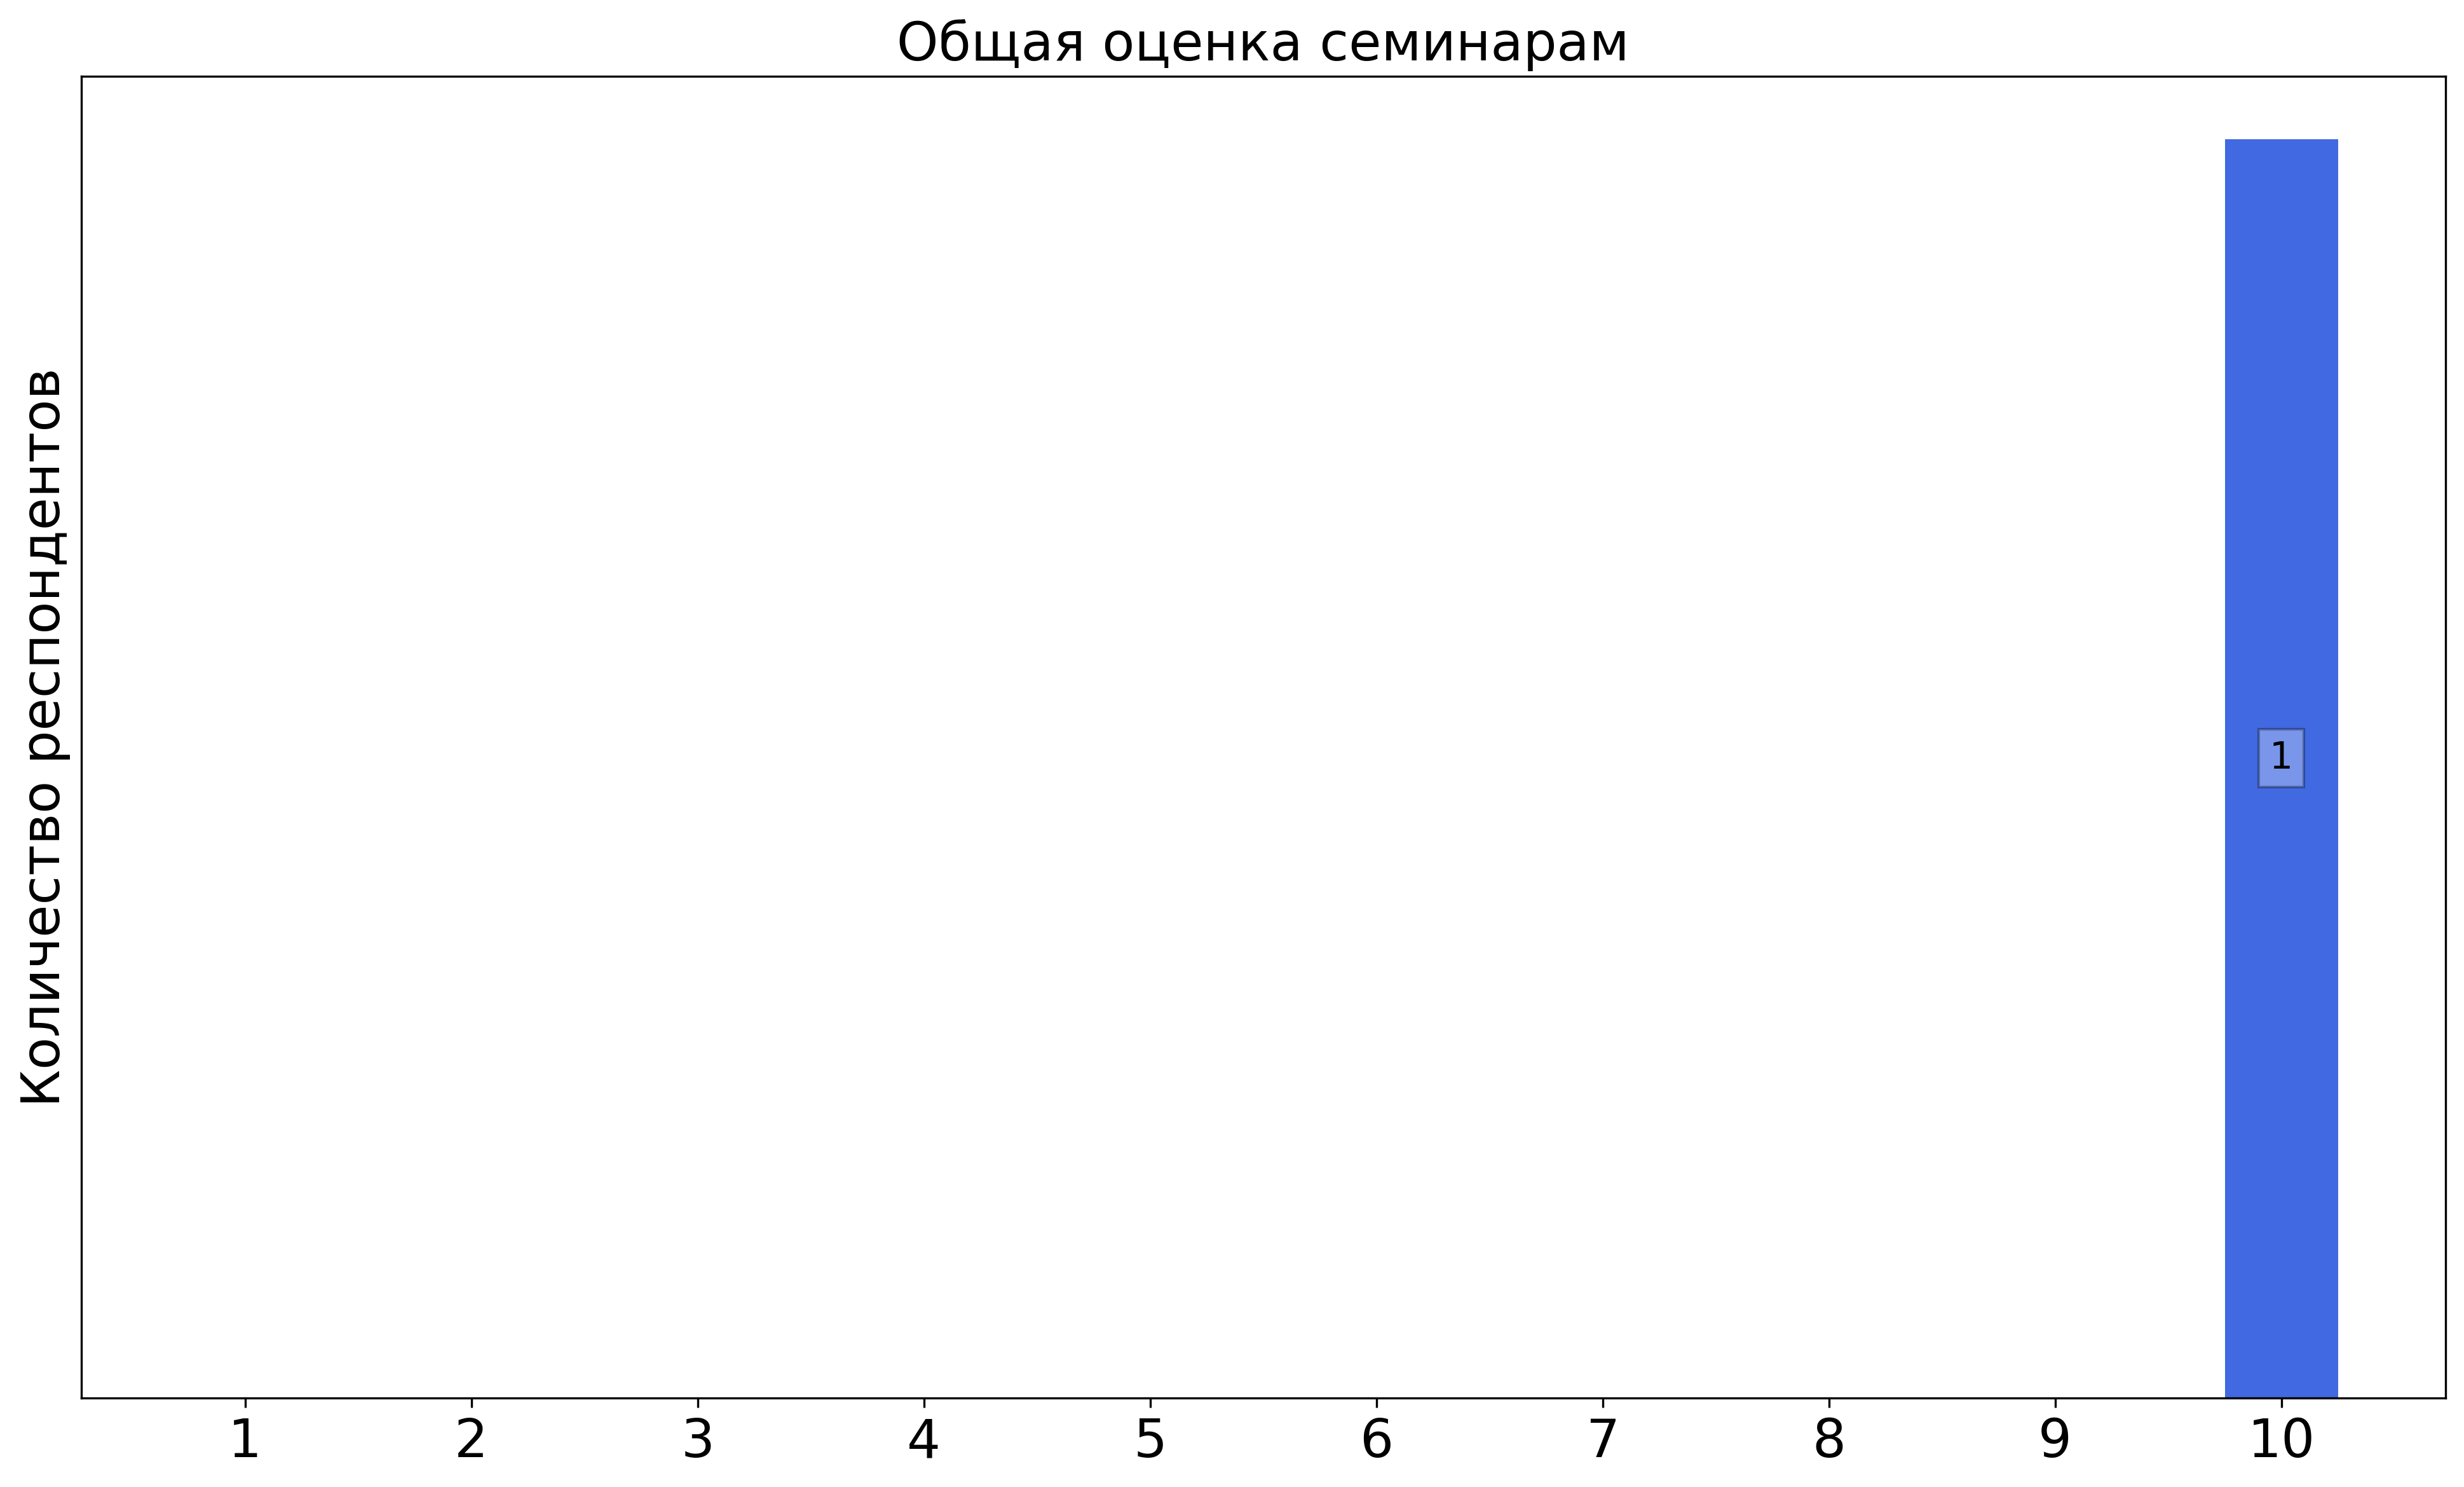
\includegraphics[width=\textwidth]{images/4 course/Защита информации/seminarists-marks-Григорьев И.А.-3.png}
            \end{subfigure}	
            \caption{Оценки респондентов о качестве преподавания семинаров}
        \end{figure}


          
    \subsubsection{Отзыв студентов о семинарах. Семинарист: Колыбельников А.И.}
        \begin{figure}[H]
            \centering
            \begin{subfigure}[b]{0.45\textwidth}
                \centering
                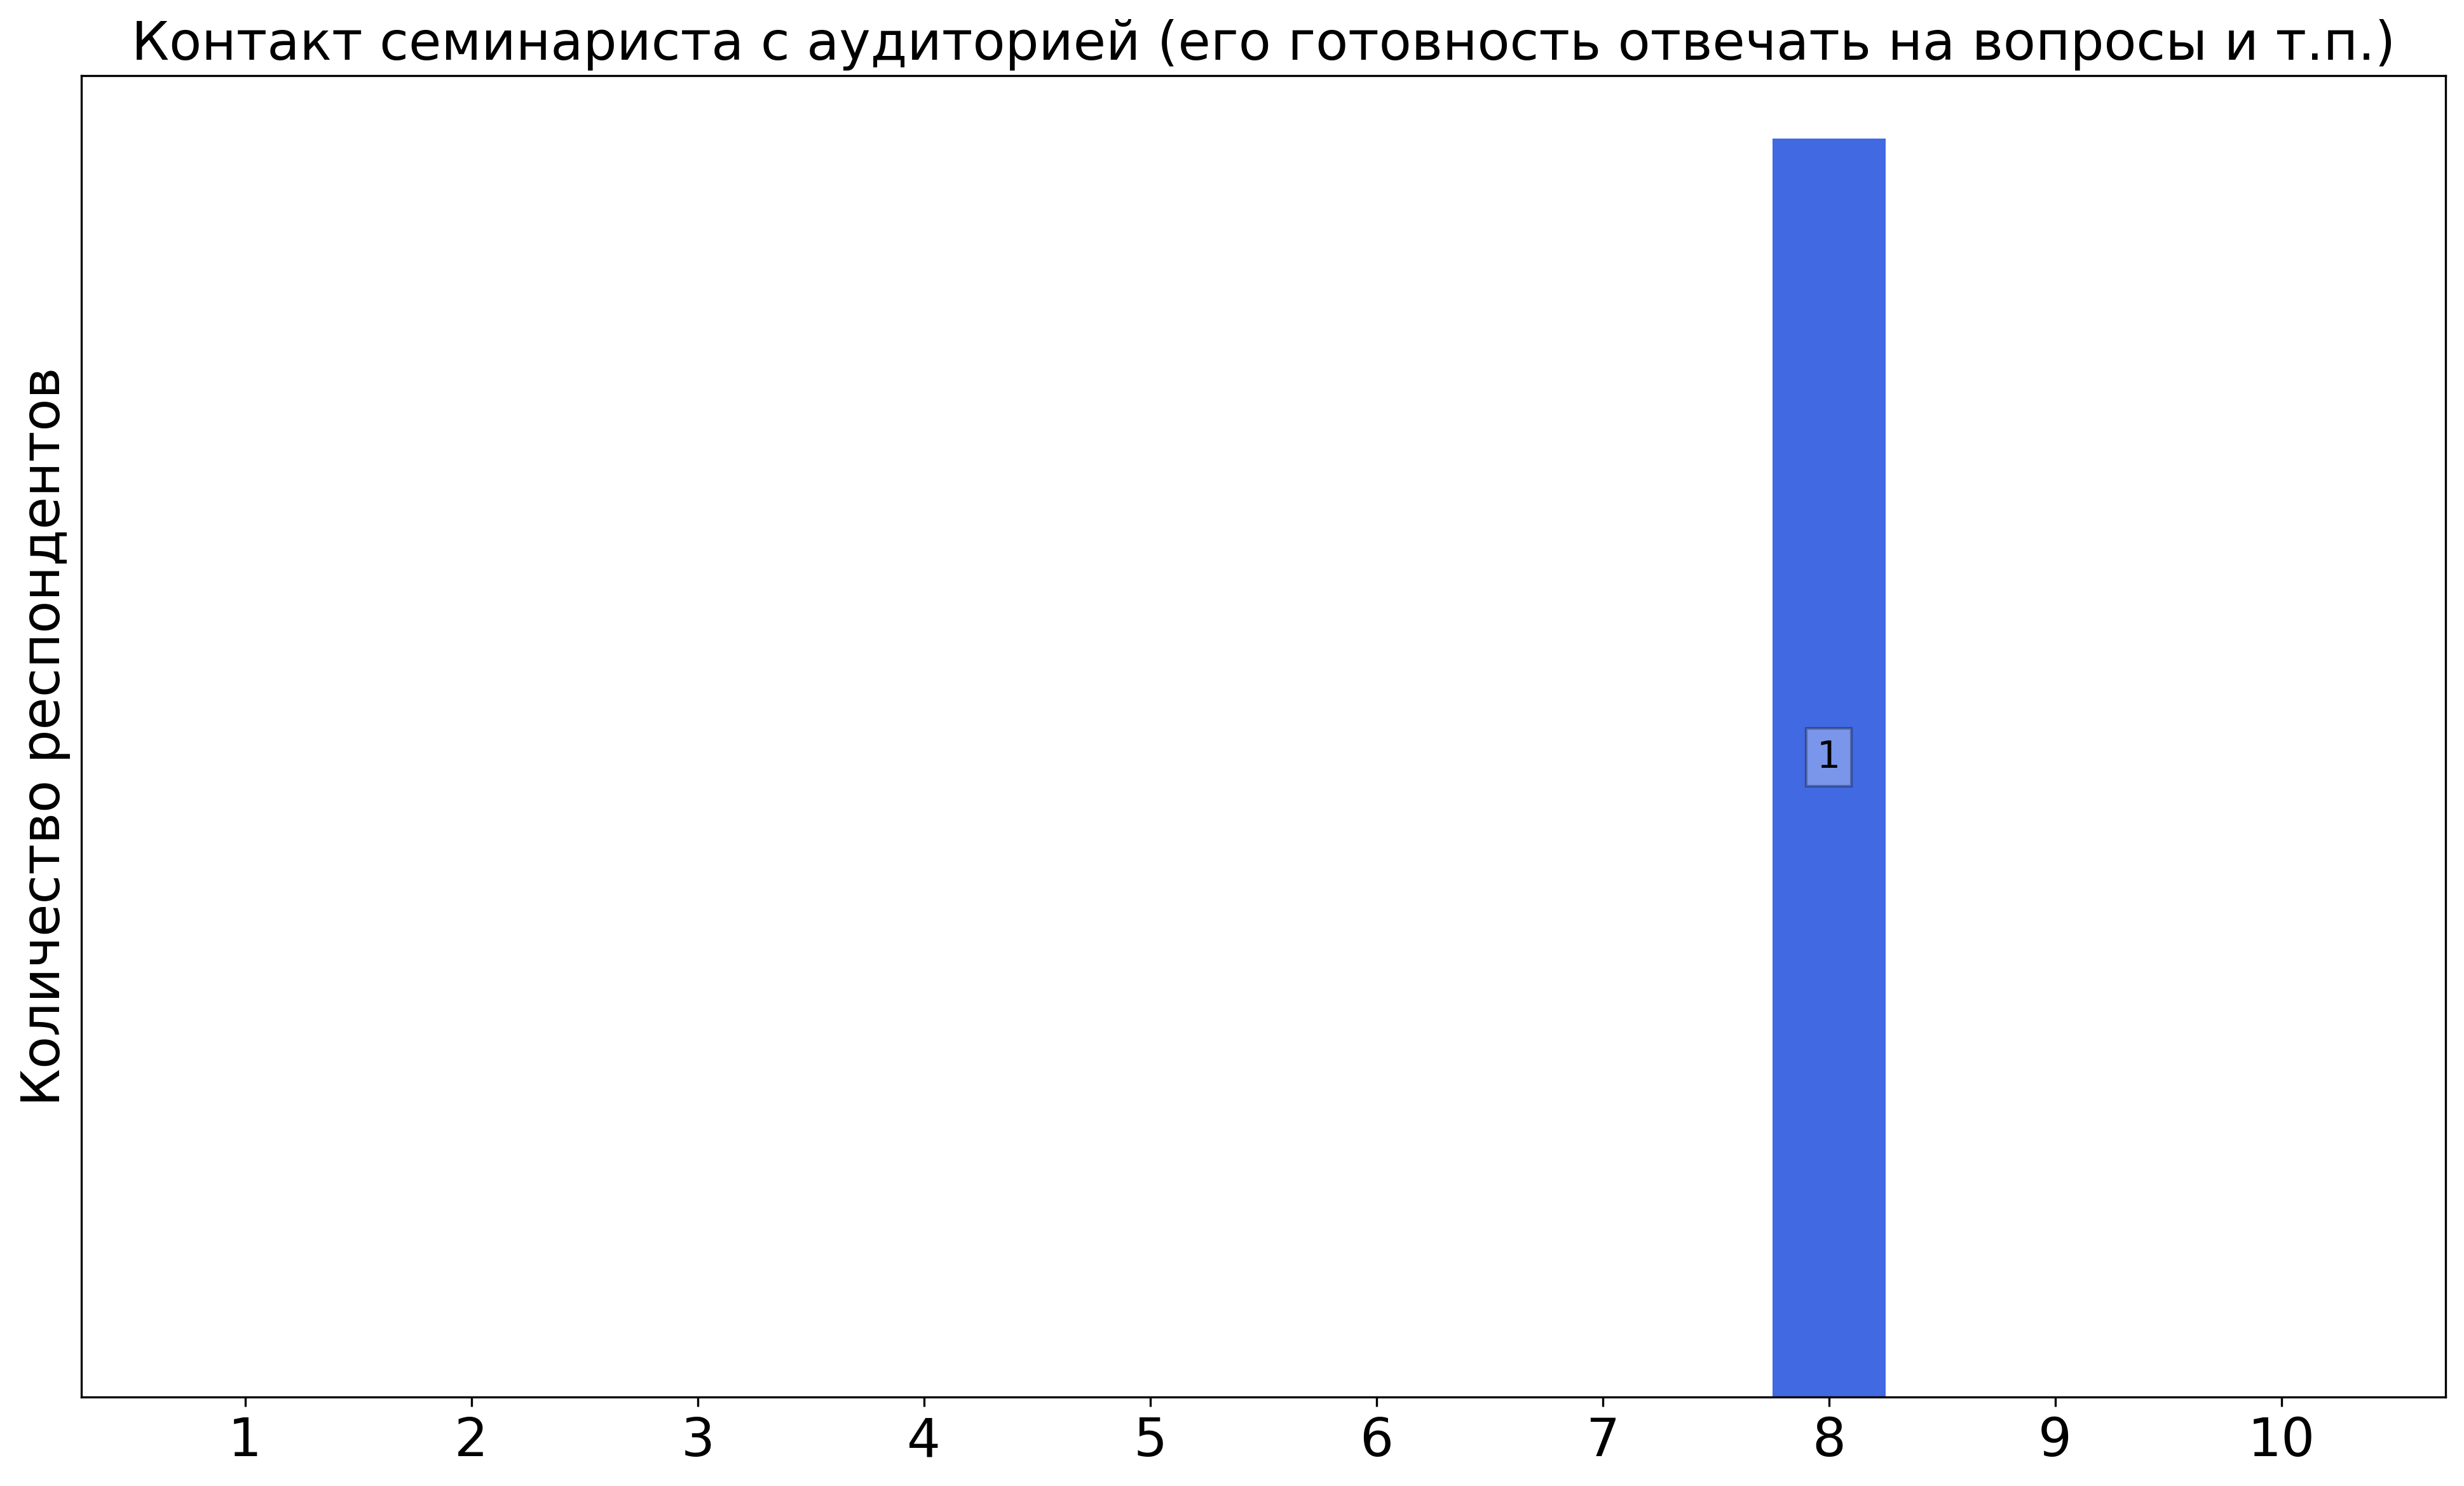
\includegraphics[width=\textwidth]{images/4 course/Защита информации/seminarists-marks-Колыбельников А.И.-0.png}
            \end{subfigure}
            \begin{subfigure}[b]{0.45\textwidth}
                \centering
                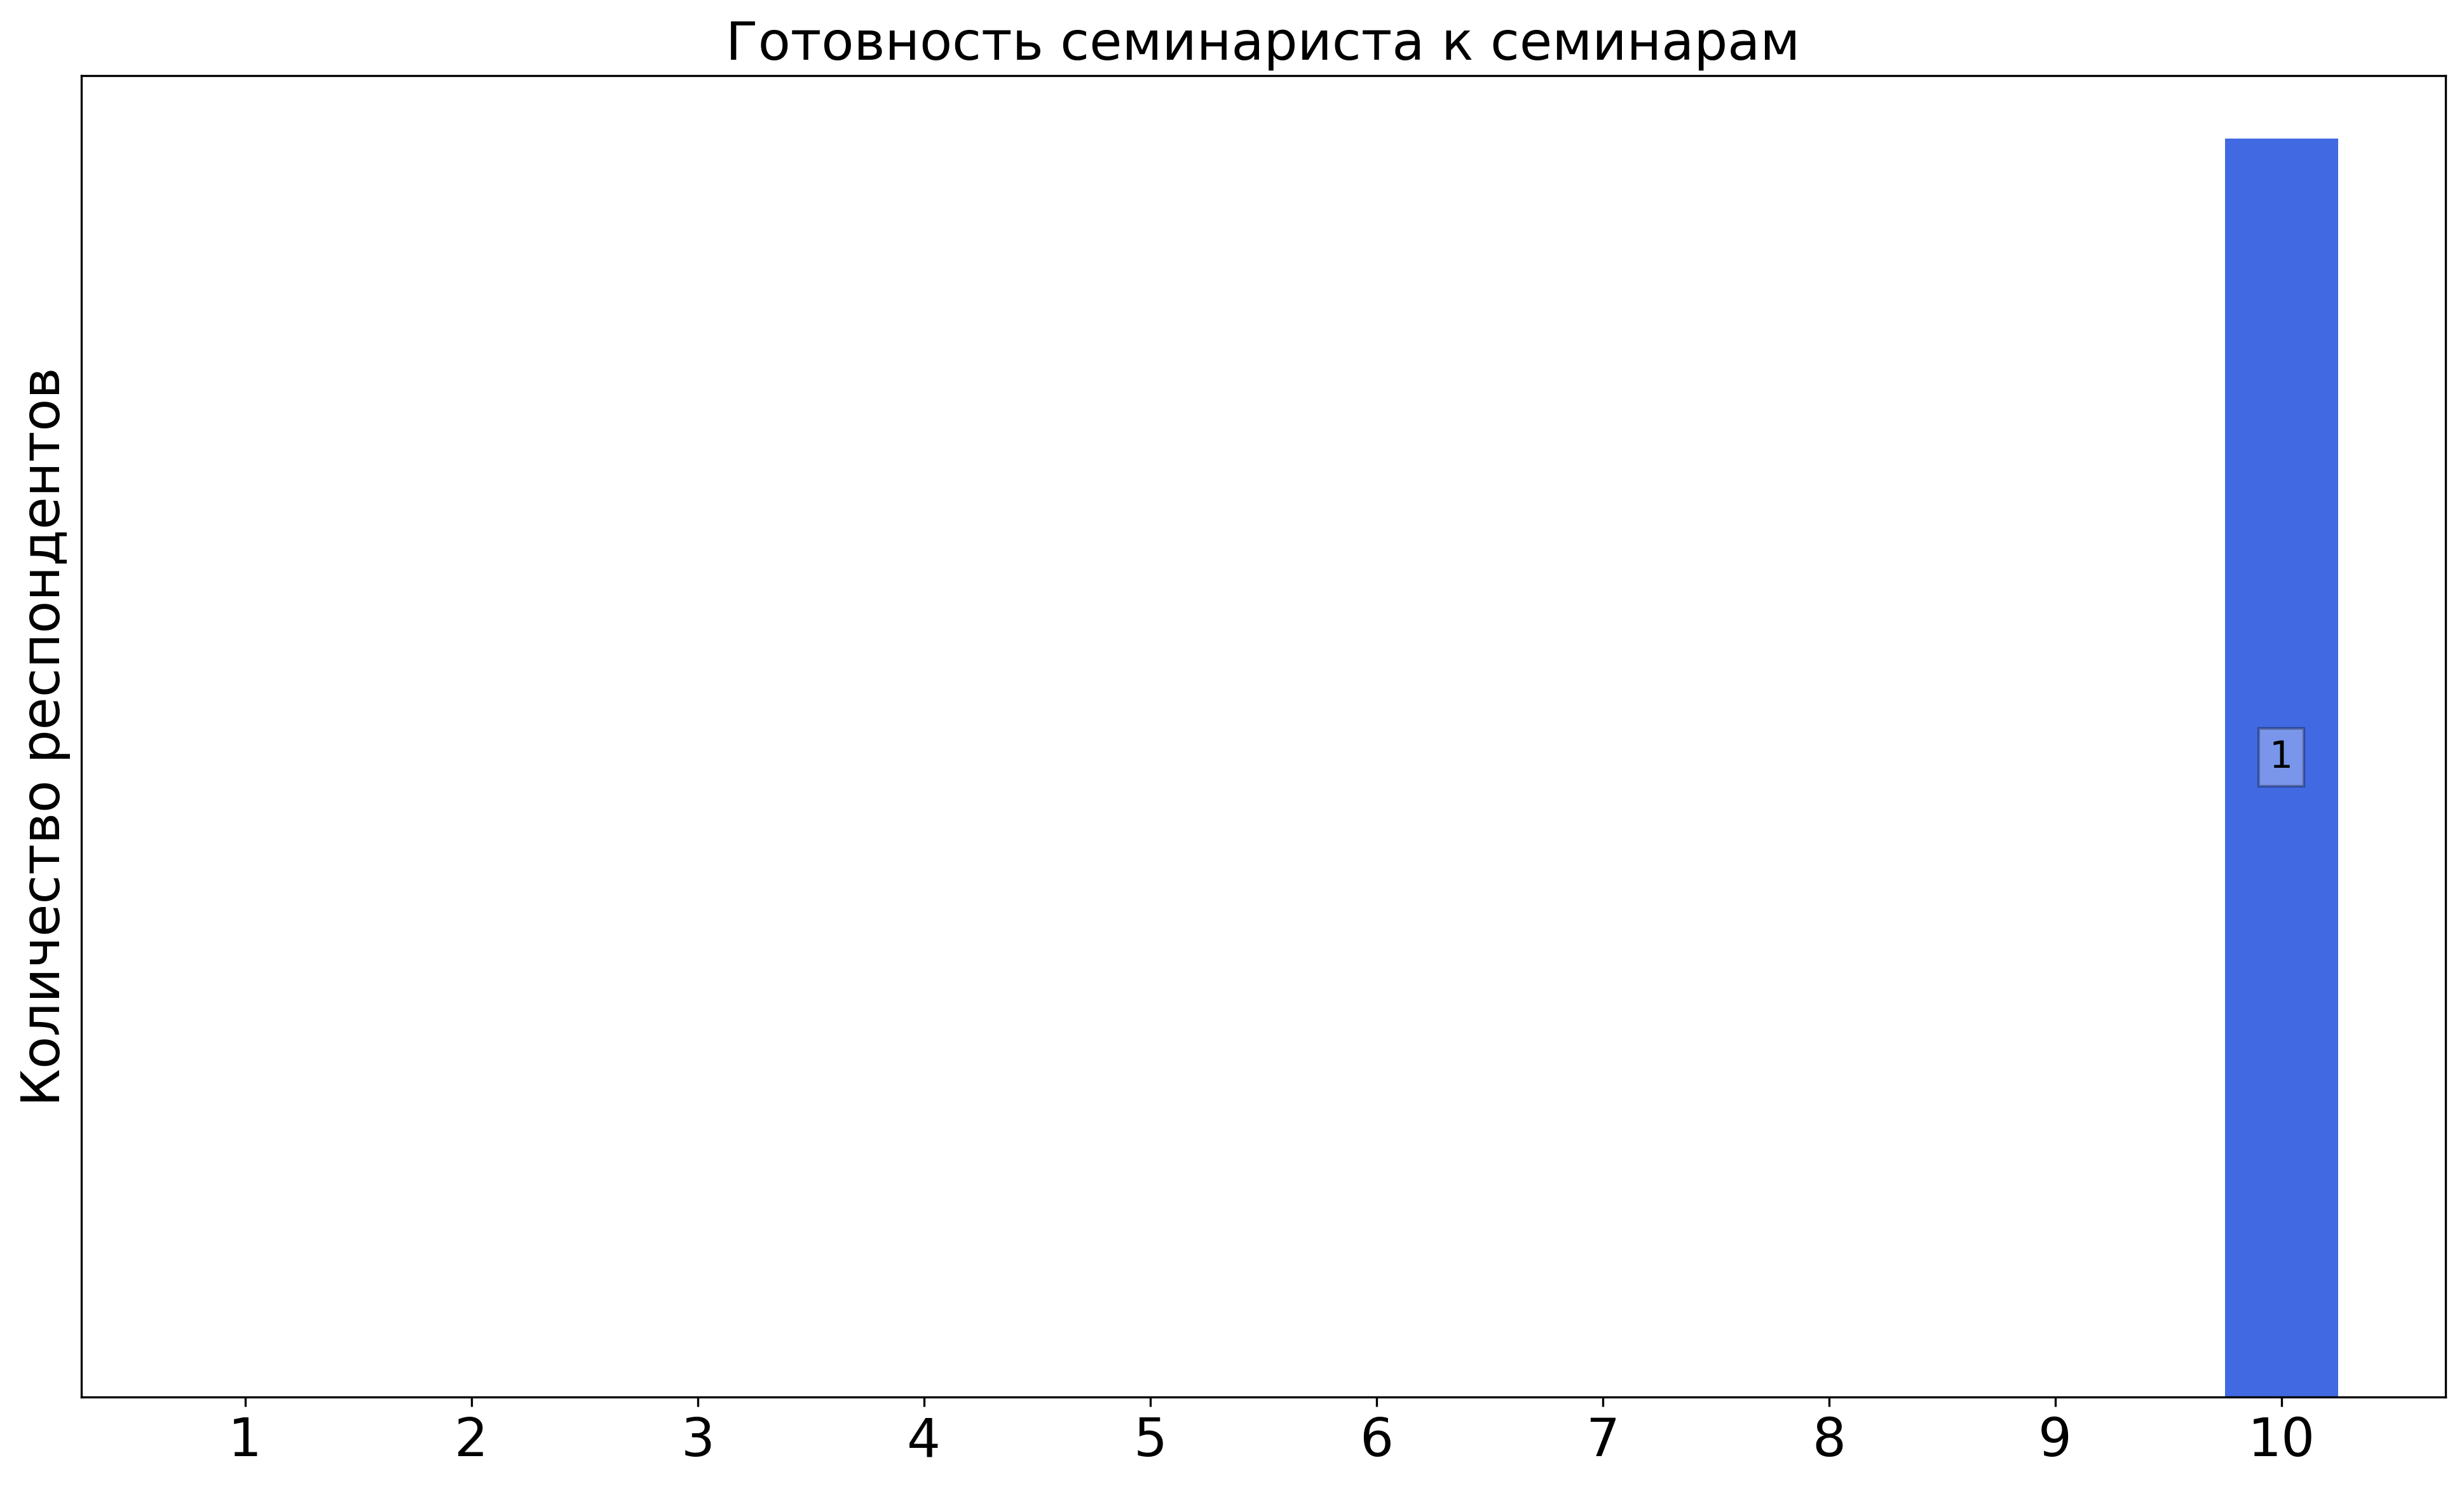
\includegraphics[width=\textwidth]{images/4 course/Защита информации/seminarists-marks-Колыбельников А.И.-1.png}
            \end{subfigure}
            \begin{subfigure}[b]{0.45\textwidth}
                \centering
                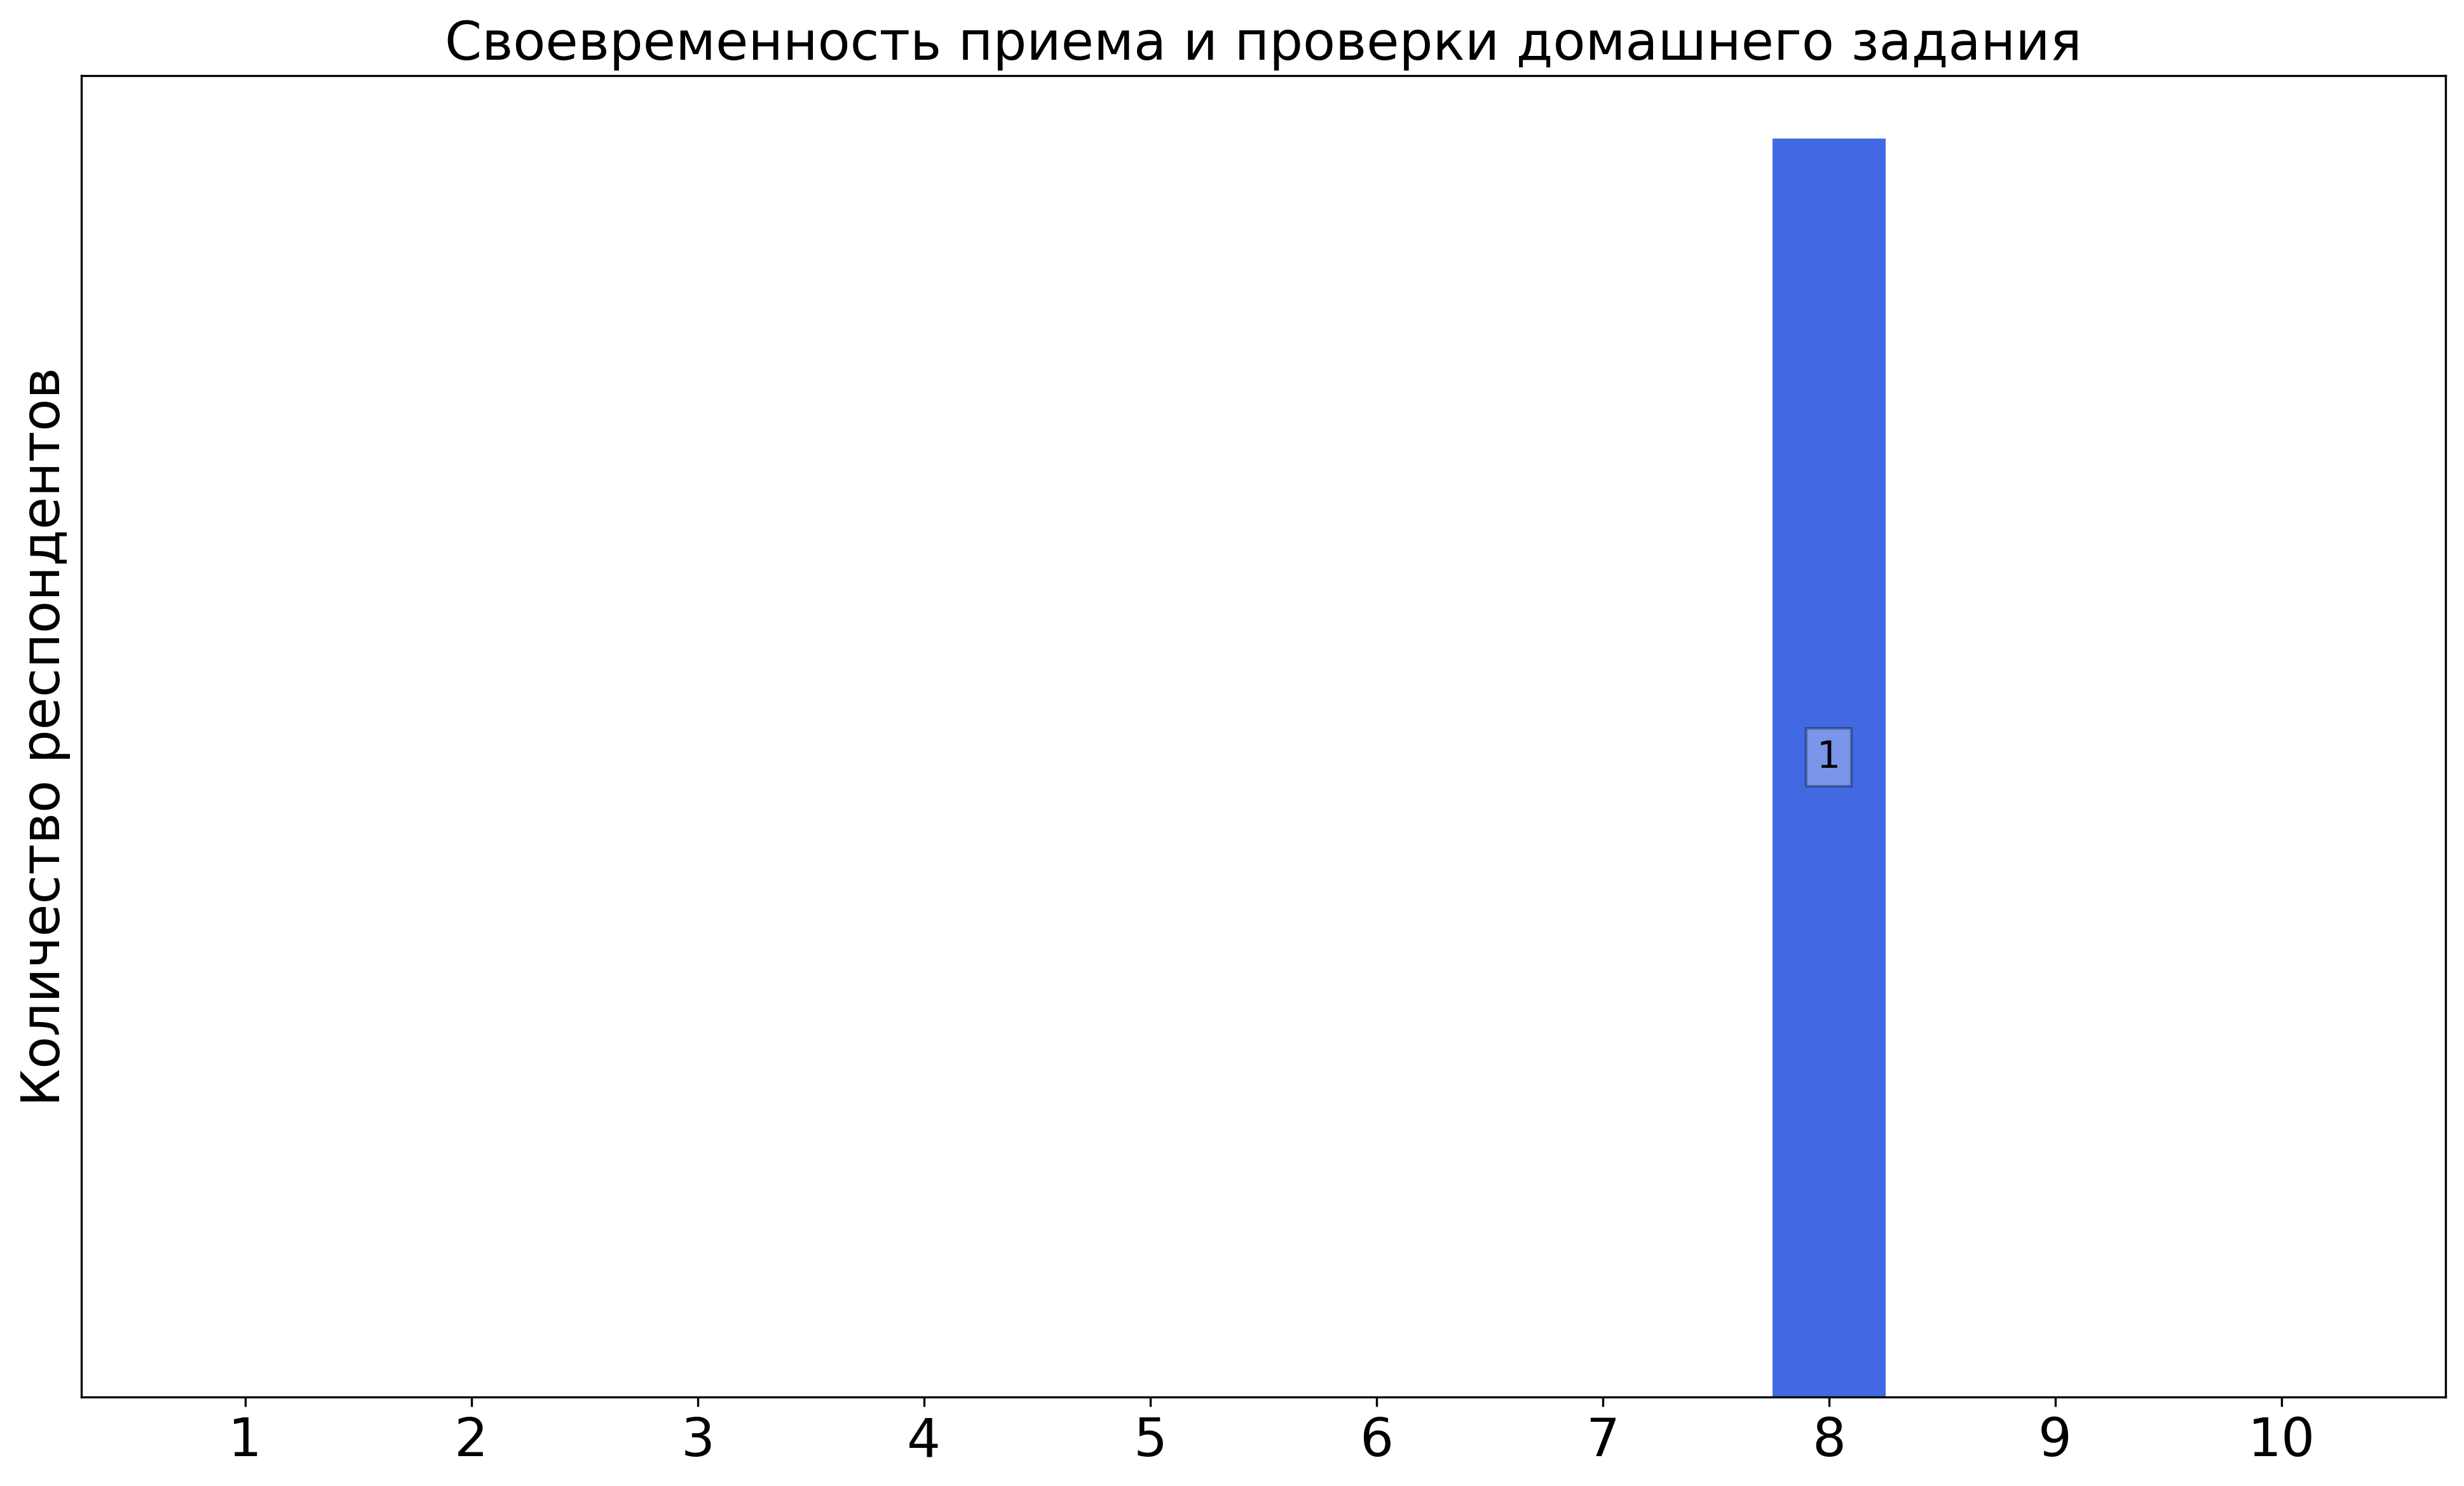
\includegraphics[width=\textwidth]{images/4 course/Защита информации/seminarists-marks-Колыбельников А.И.-2.png}
            \end{subfigure}
            \begin{subfigure}[b]{0.45\textwidth}
                \centering
                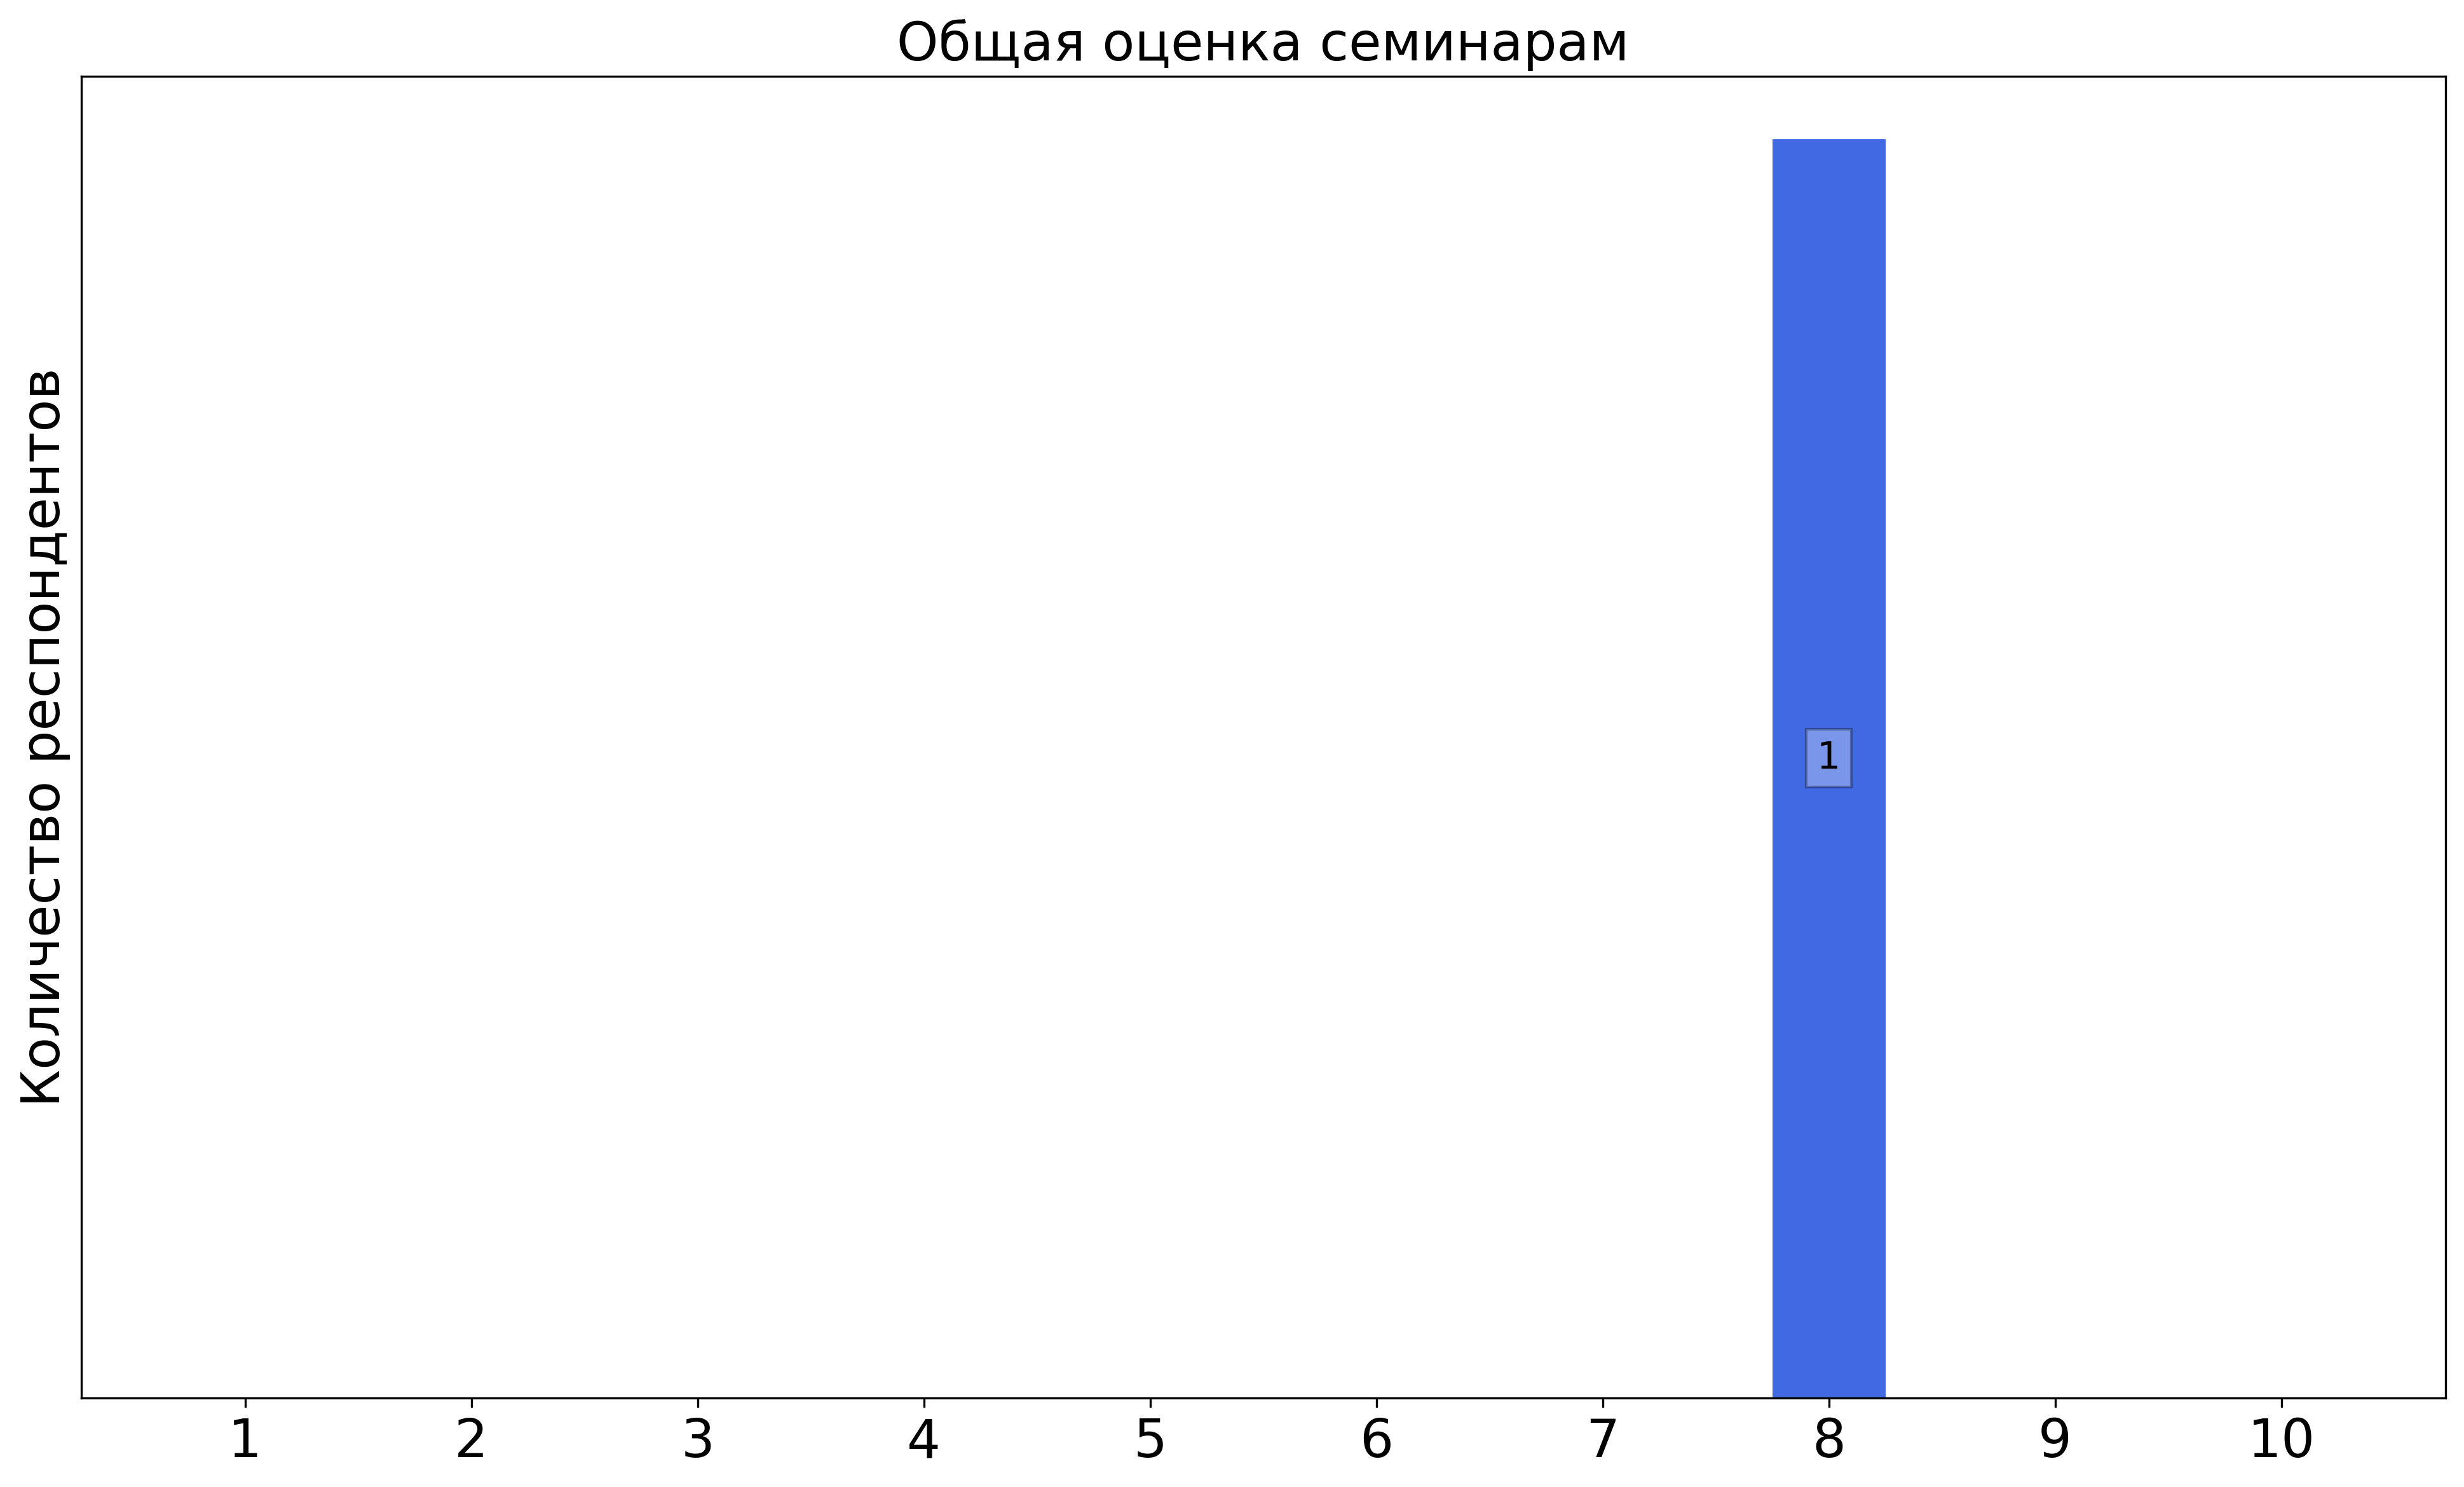
\includegraphics[width=\textwidth]{images/4 course/Защита информации/seminarists-marks-Колыбельников А.И.-3.png}
            \end{subfigure}	
            \caption{Оценки респондентов о качестве преподавания семинаров}
        \end{figure}

  
    \subsubsection{Отзыв студентов о семинарах. Семинарист: Мозолина Н.В.}
		\begin{figure}[H]
			\centering
			\begin{subfigure}[b]{0.45\textwidth}
				\centering
				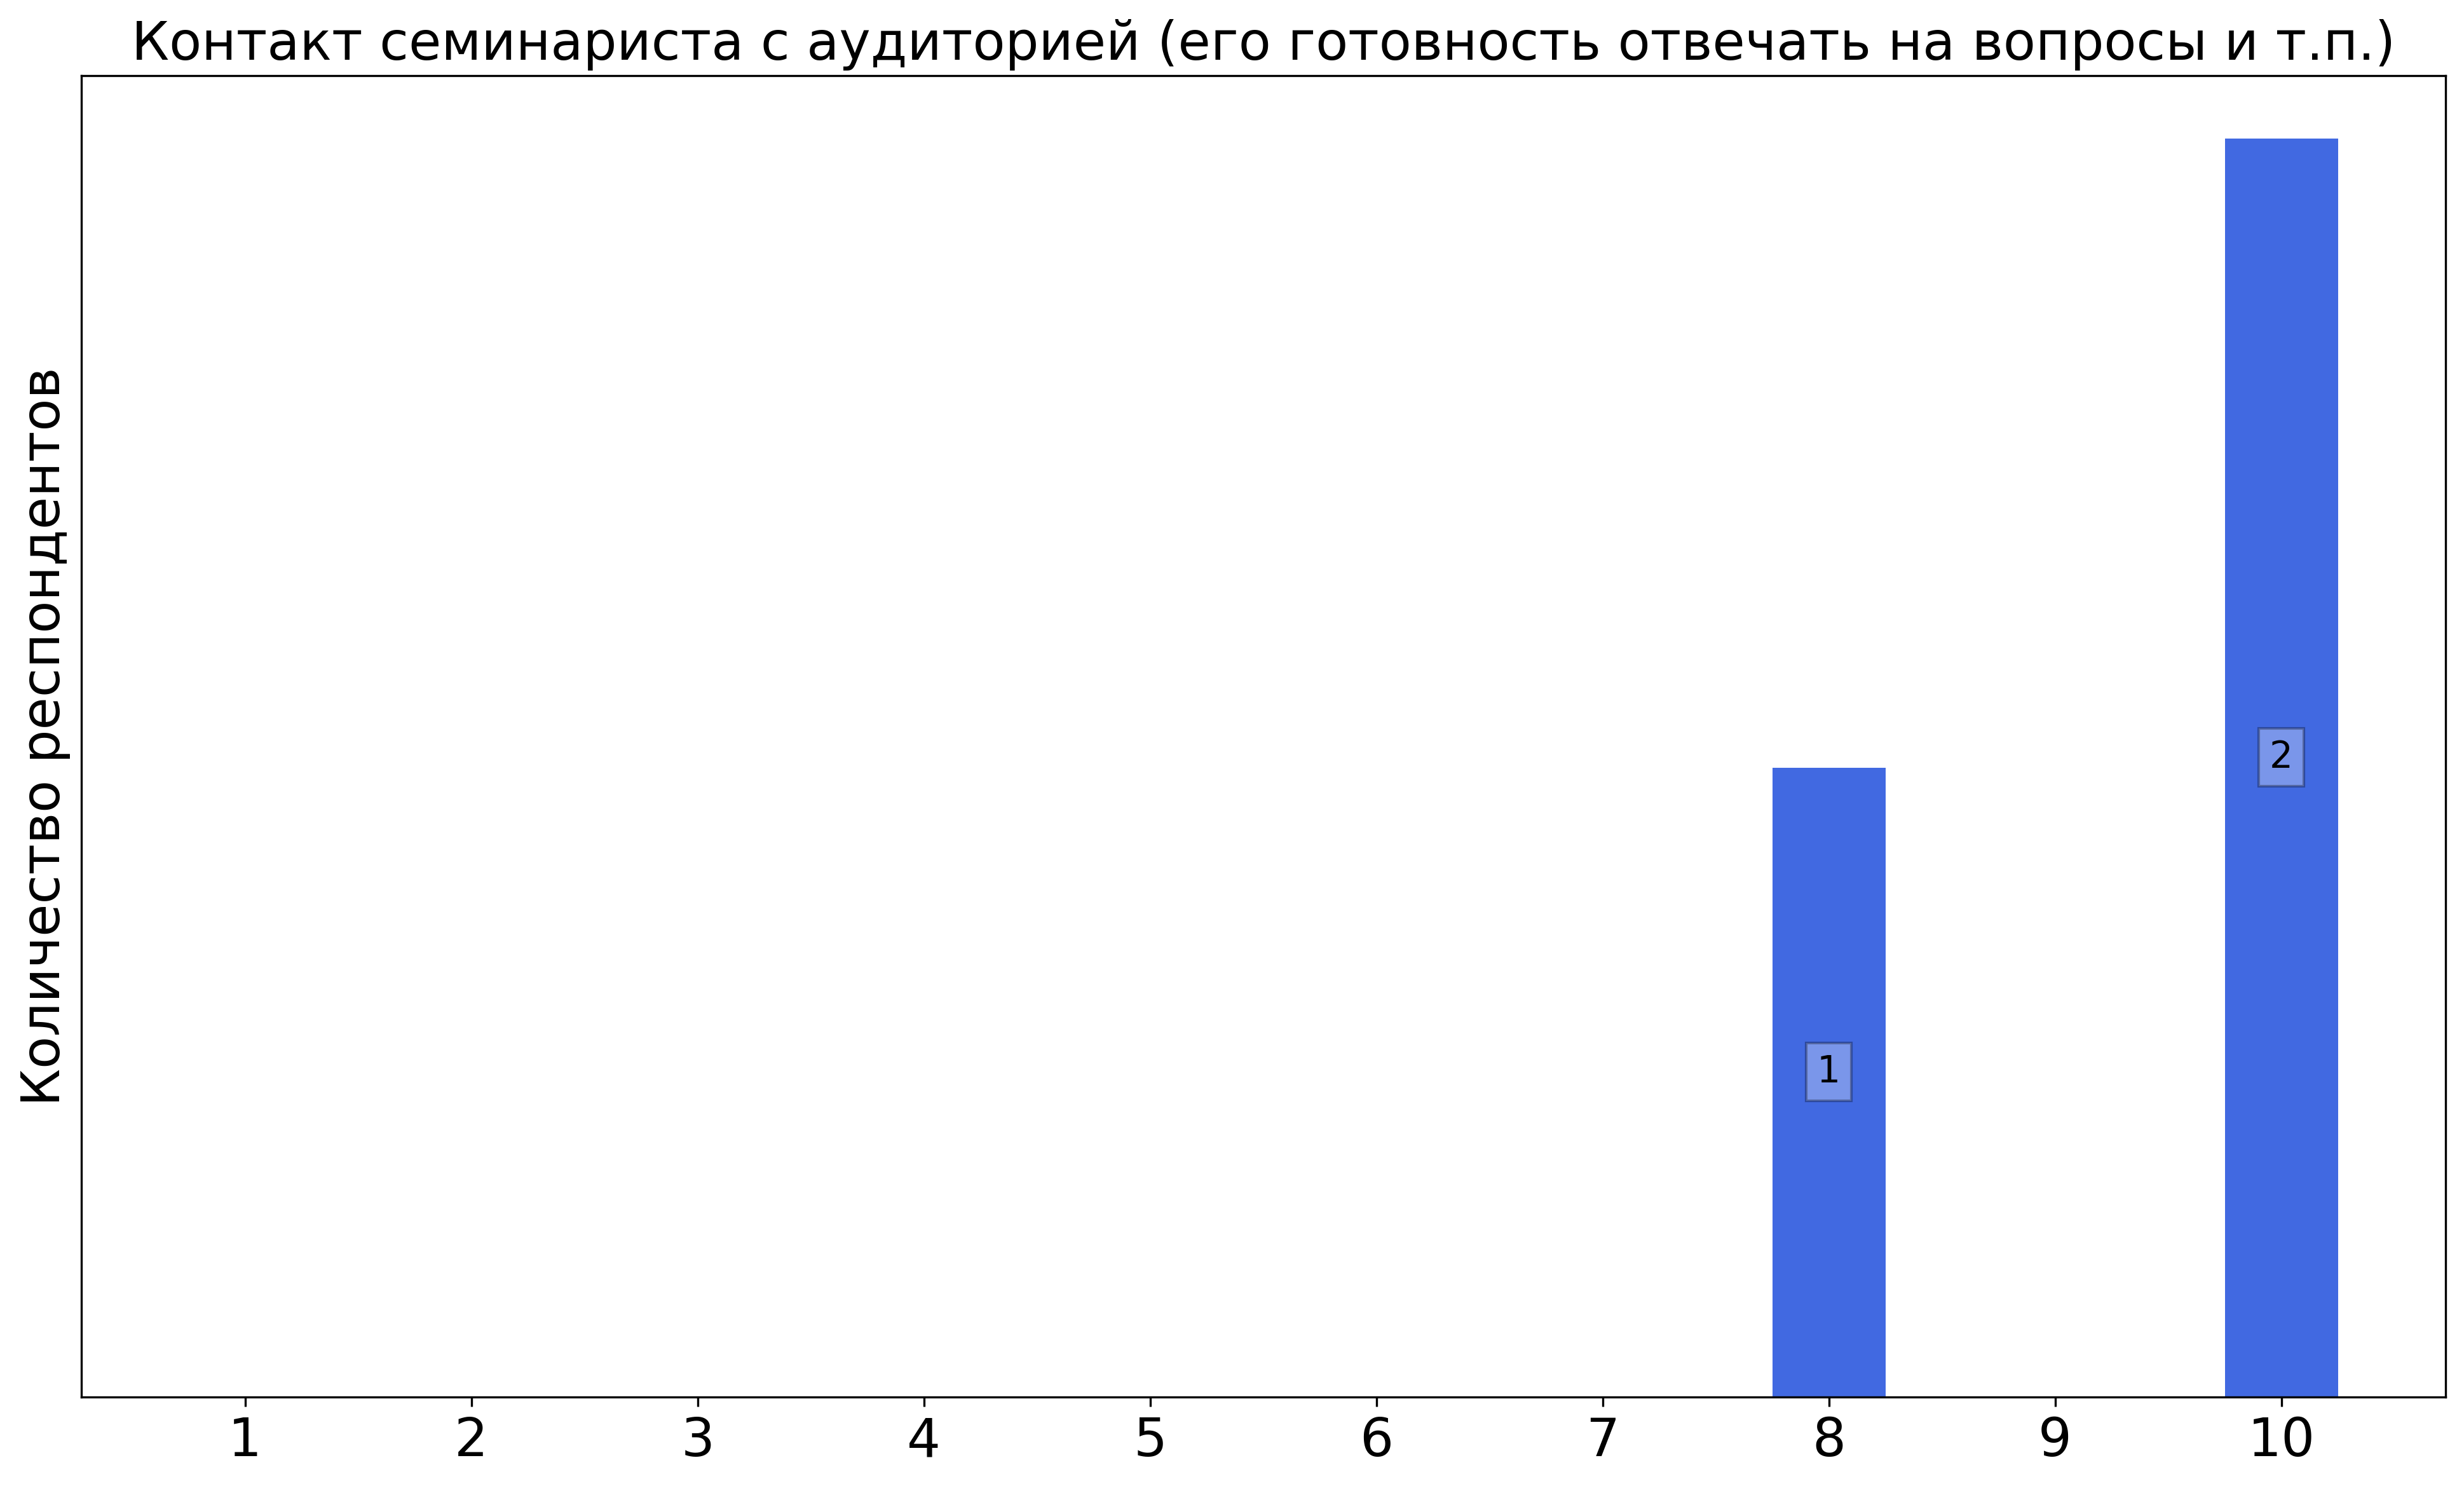
\includegraphics[width=\textwidth]{images/4 course/Защита информации/seminarists-marks-Мозолина Н.В.-0.png}
			\end{subfigure}
			\begin{subfigure}[b]{0.45\textwidth}
				\centering
				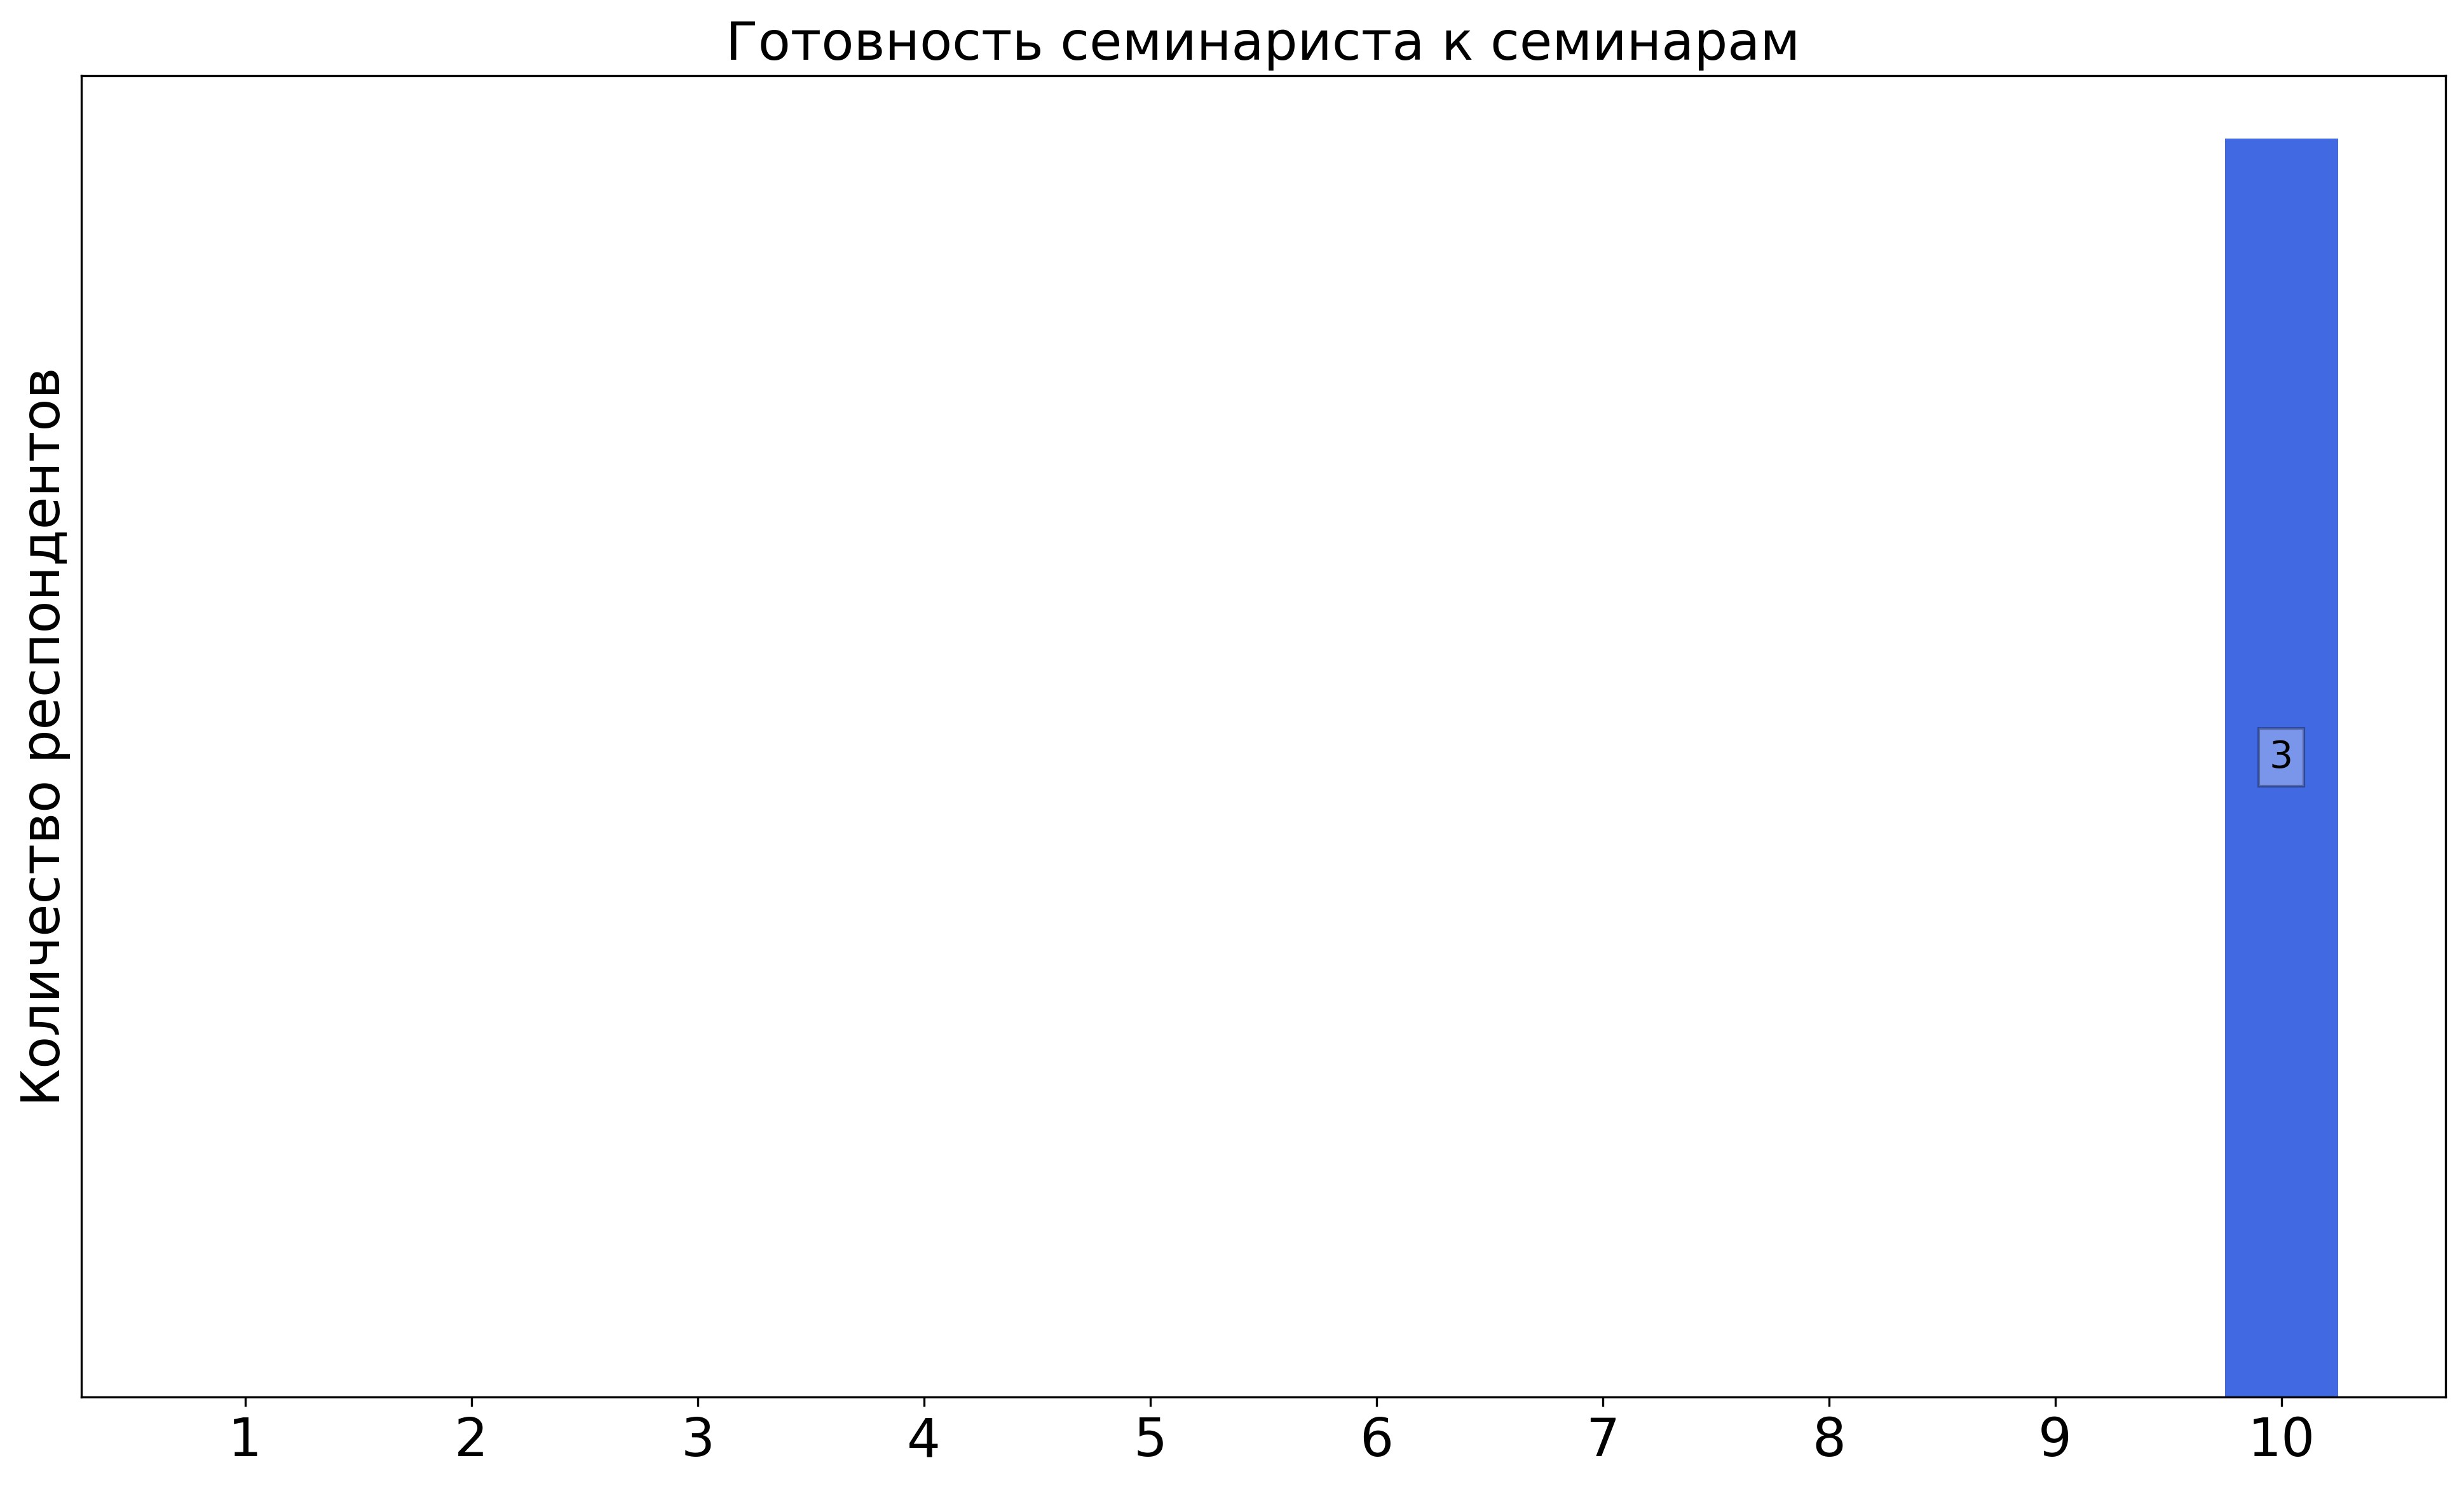
\includegraphics[width=\textwidth]{images/4 course/Защита информации/seminarists-marks-Мозолина Н.В.-1.png}
			\end{subfigure}
			\begin{subfigure}[b]{0.45\textwidth}
				\centering
				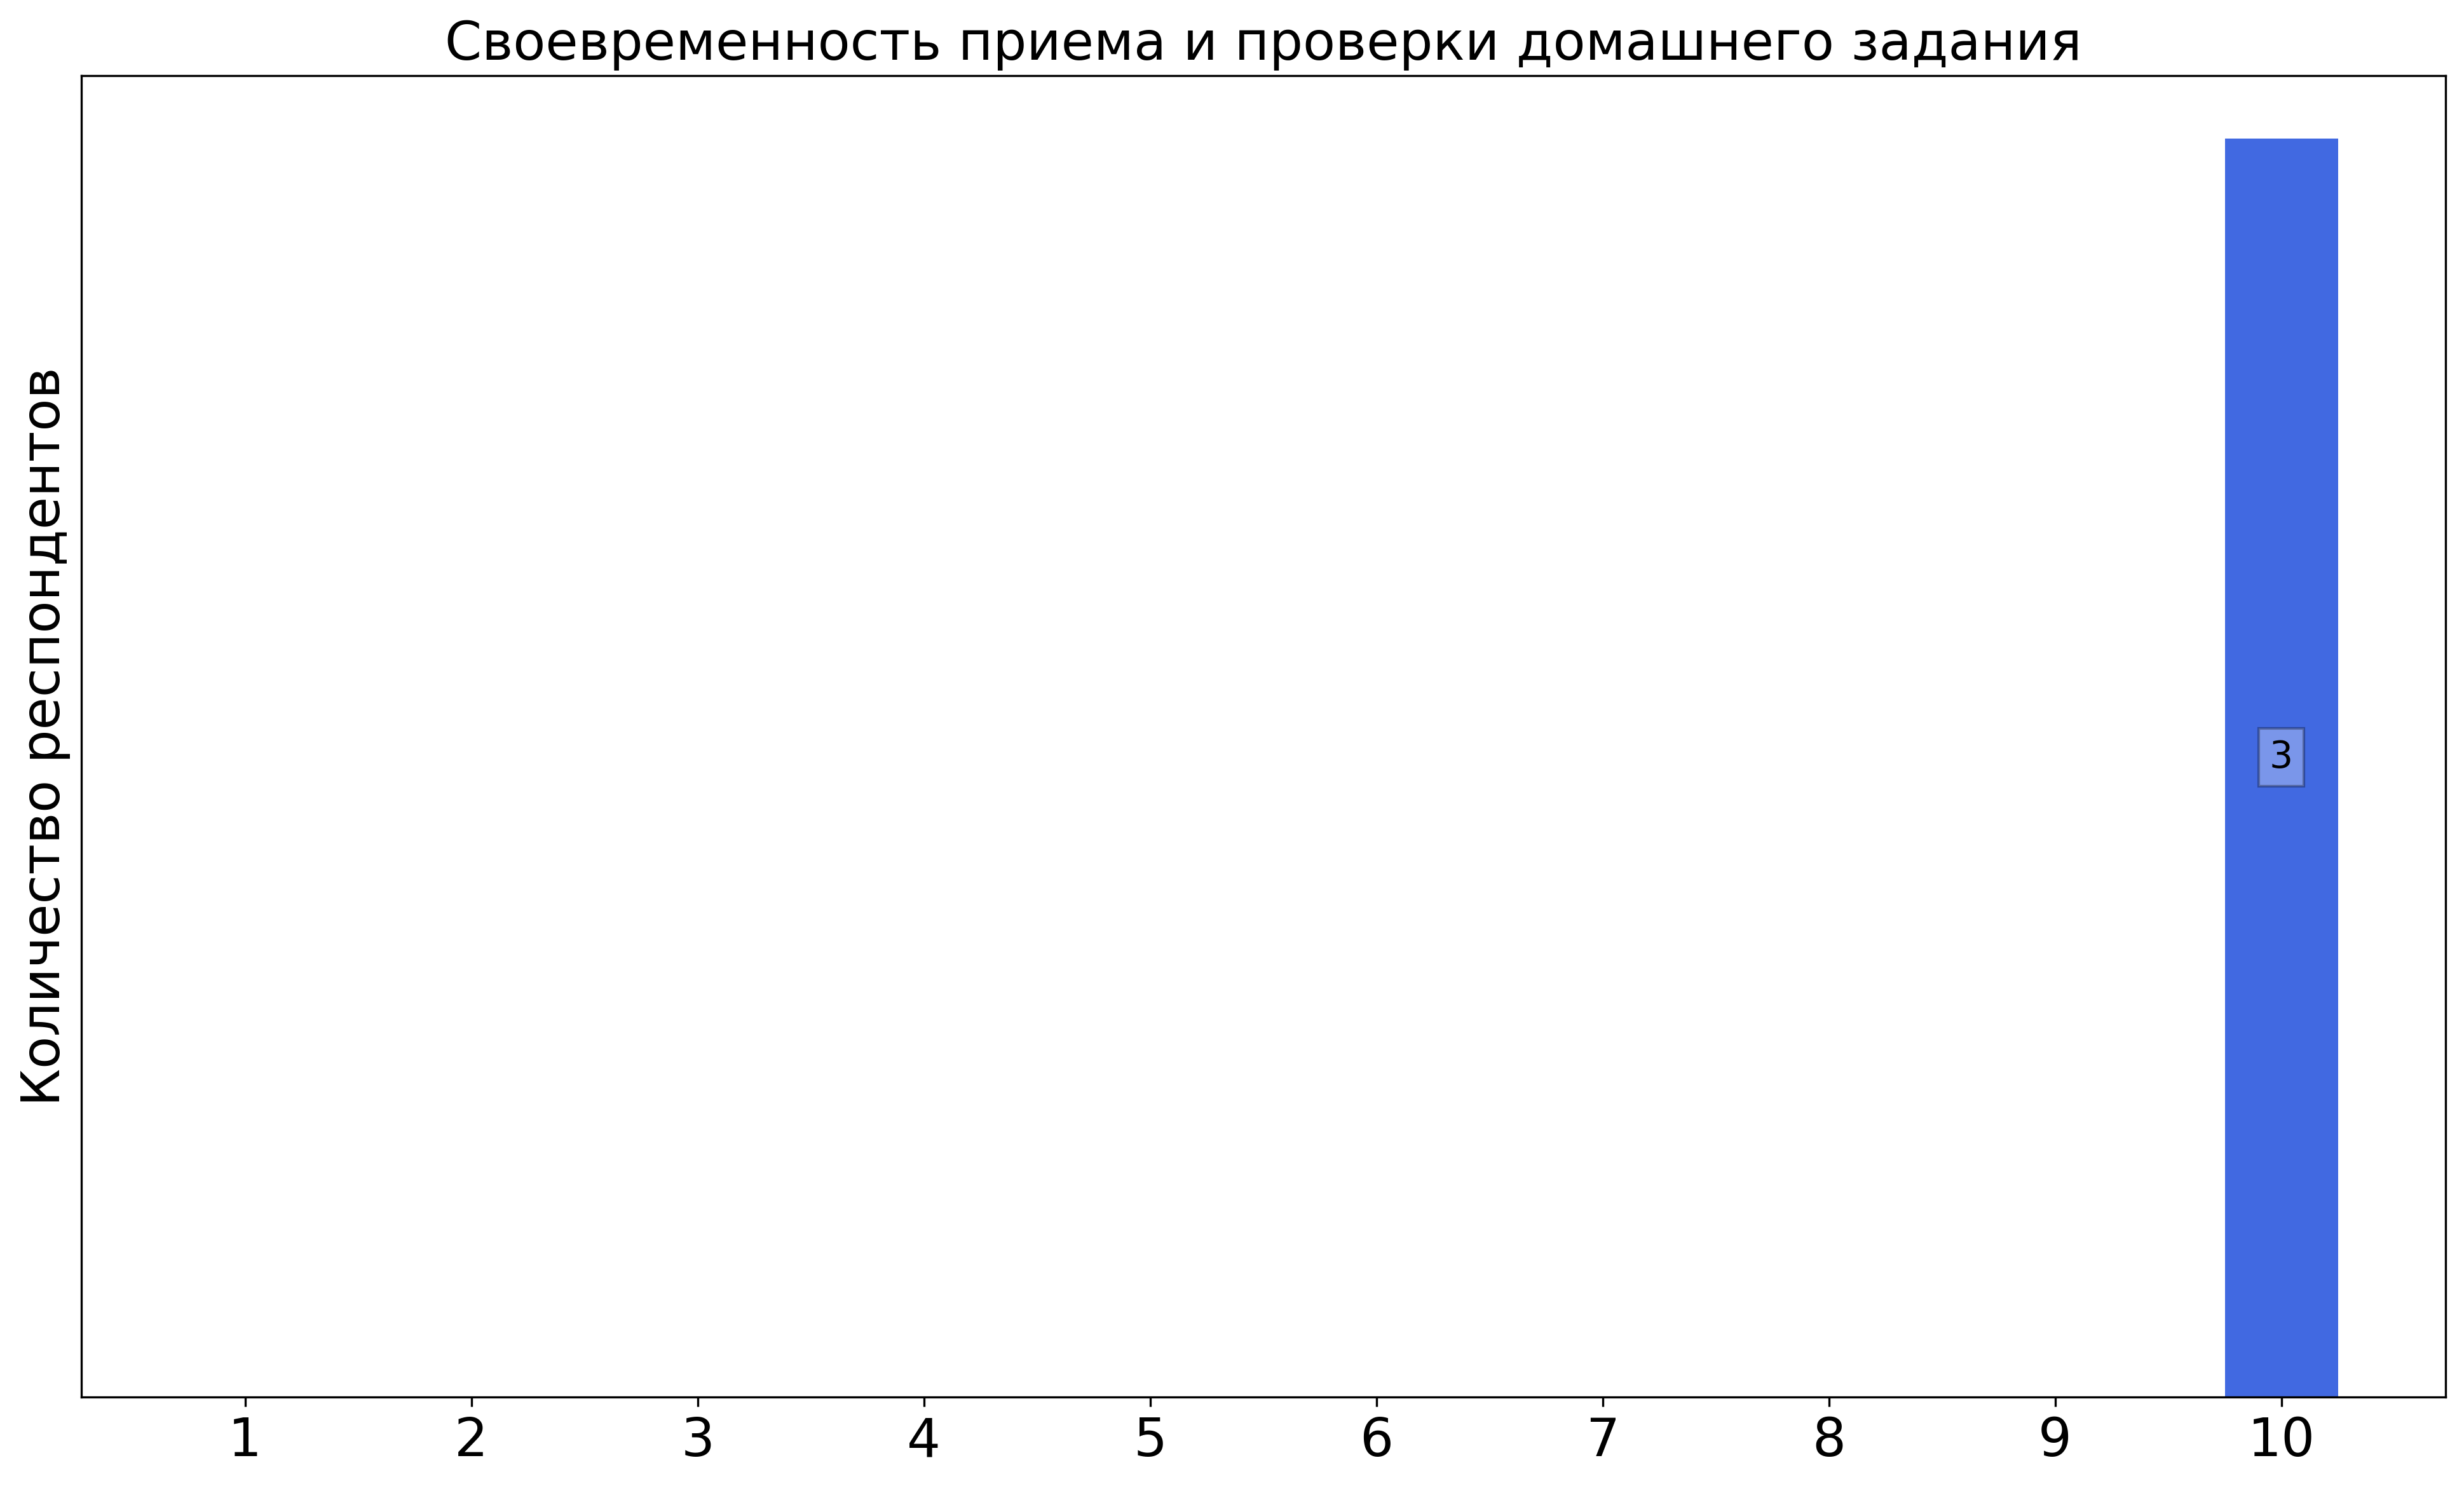
\includegraphics[width=\textwidth]{images/4 course/Защита информации/seminarists-marks-Мозолина Н.В.-2.png}
			\end{subfigure}
			\begin{subfigure}[b]{0.45\textwidth}
				\centering
				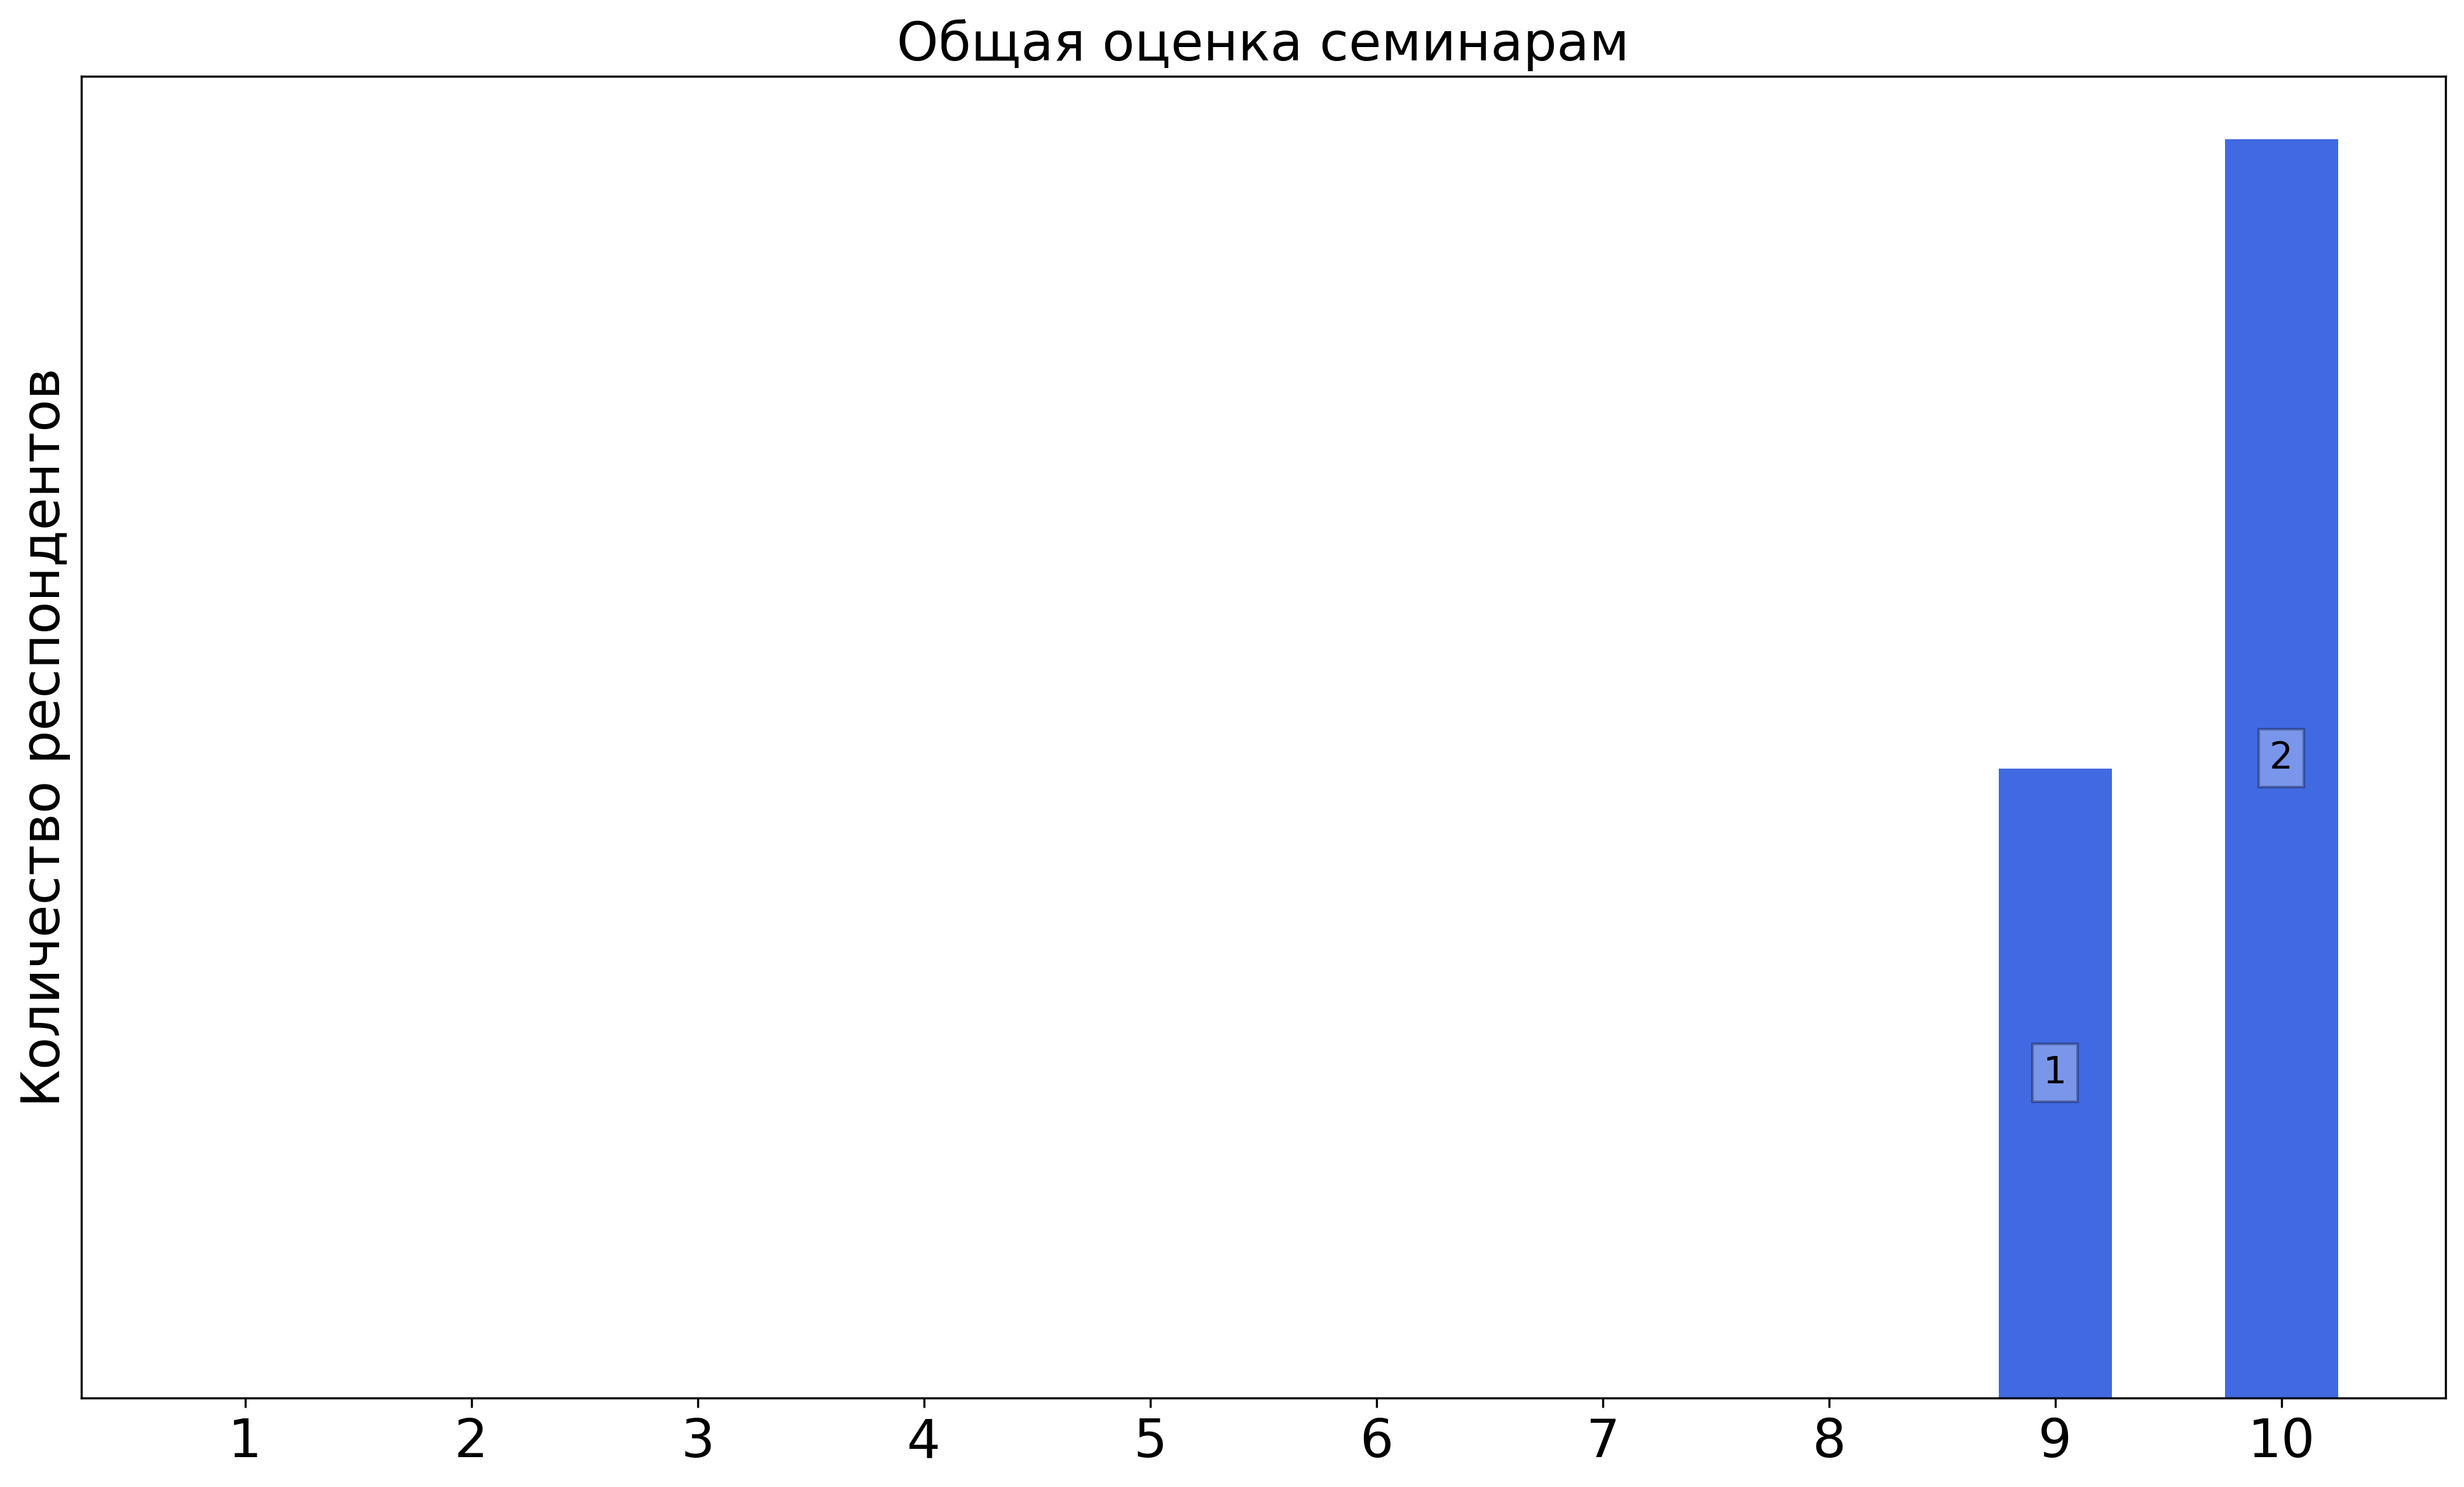
\includegraphics[width=\textwidth]{images/4 course/Защита информации/seminarists-marks-Мозолина Н.В.-3.png}
			\end{subfigure}	
			\caption{Оценки респондентов о качестве преподавания семинаров}
		\end{figure}

		\textbf{Комментарии студентов о семинаристе\protect\footnote{сохранены оригинальные орфография и пунктуация}}
            \begin{commentbox} 
                Оценивала сильно строже, чем другие семинаристы. То есть соблюдала абсолютно все формальности, но как человек и как преподаватель нет вопросов 
            \end{commentbox} 
        
            \begin{commentbox} 
                Прекрасный семенарист, отлично объясняет материал 
            \end{commentbox} 
        
            \begin{commentbox} 
                Хороший семинарист. В меру строгая, разбирается в предмете. Всё выводила строго. К контрольной готовила хорошо. 
        
                Очень дотошно проверяла рефераты. На мой взгляд, плюс, так как преподаватель действительно находил ошибки и давал наводку как их исправить, а не просто принимал gpt халтуру, как  некоторые другие семинаристы. Здесь gpt работа не принималась.
        
                Впечатления только положительные  
            \end{commentbox}


    \subsubsection{Отзыв студентов о семинарах. Семинарист: Полешко А.}
        \begin{figure}[H]
            \centering
            \begin{subfigure}[b]{0.45\textwidth}
                \centering
                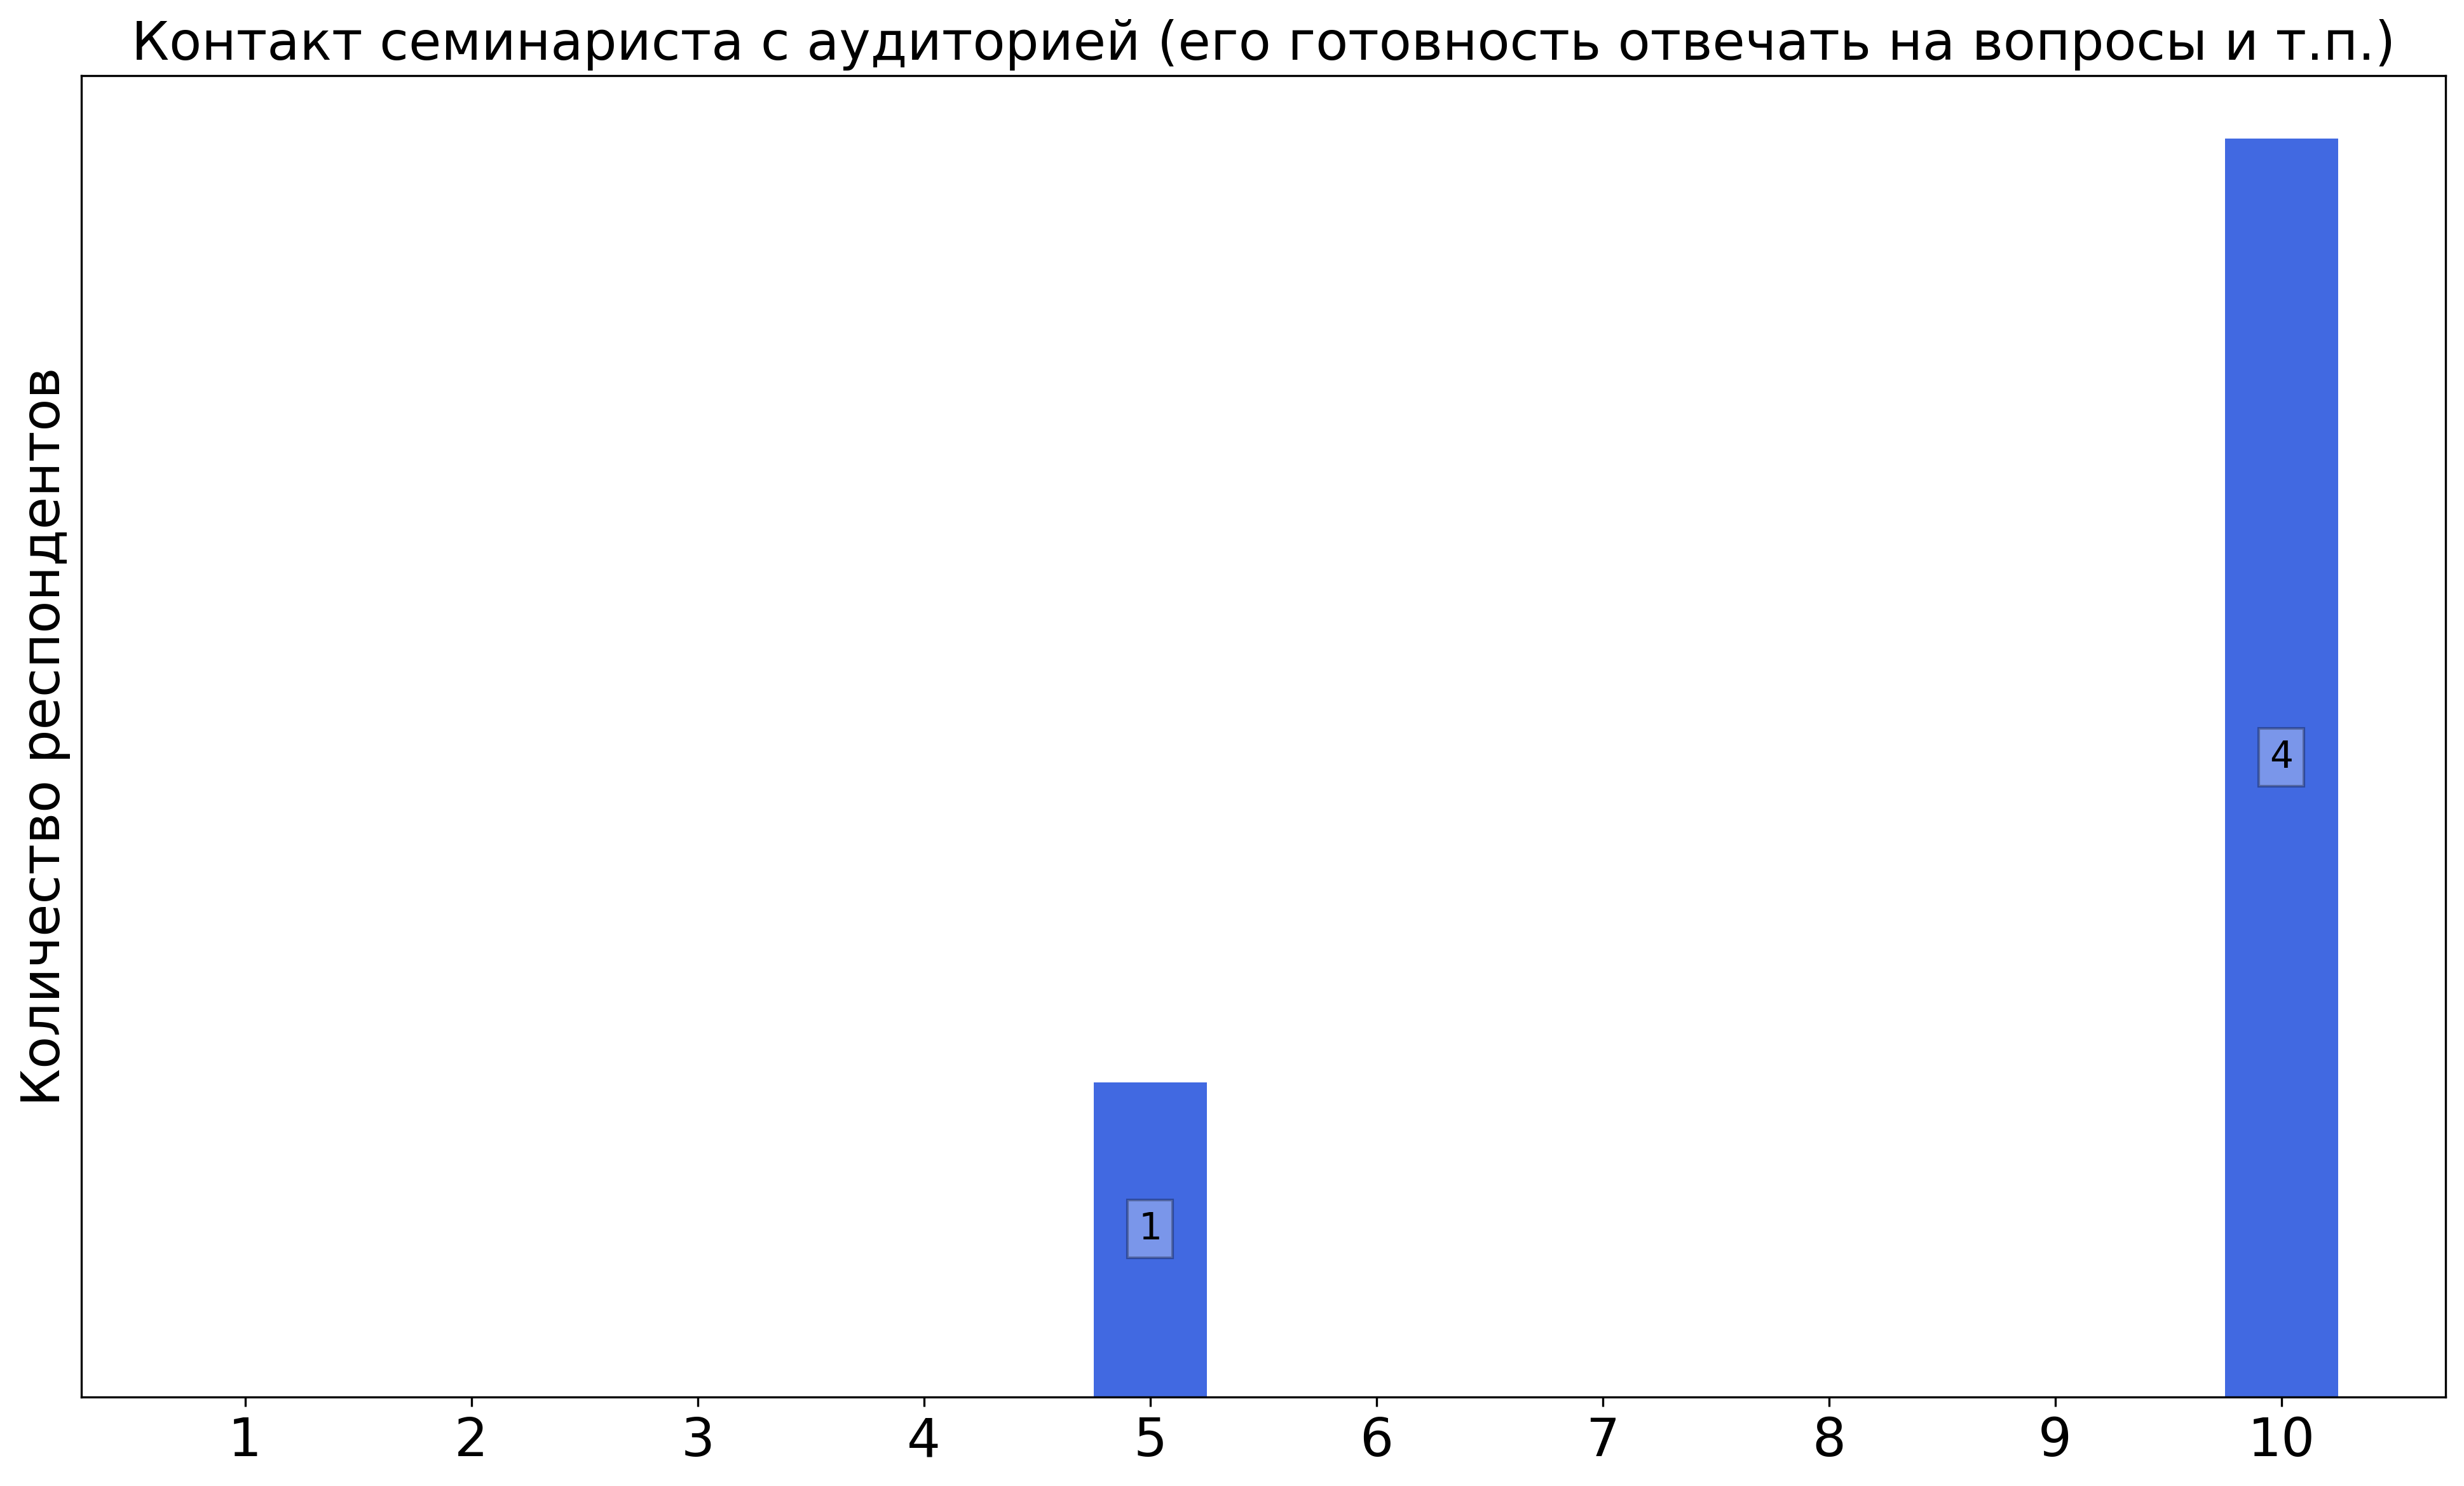
\includegraphics[width=\textwidth]{images/4 course/Защита информации/seminarists-marks-Полешко А.-0.png}
            \end{subfigure}
            \begin{subfigure}[b]{0.45\textwidth}
                \centering
                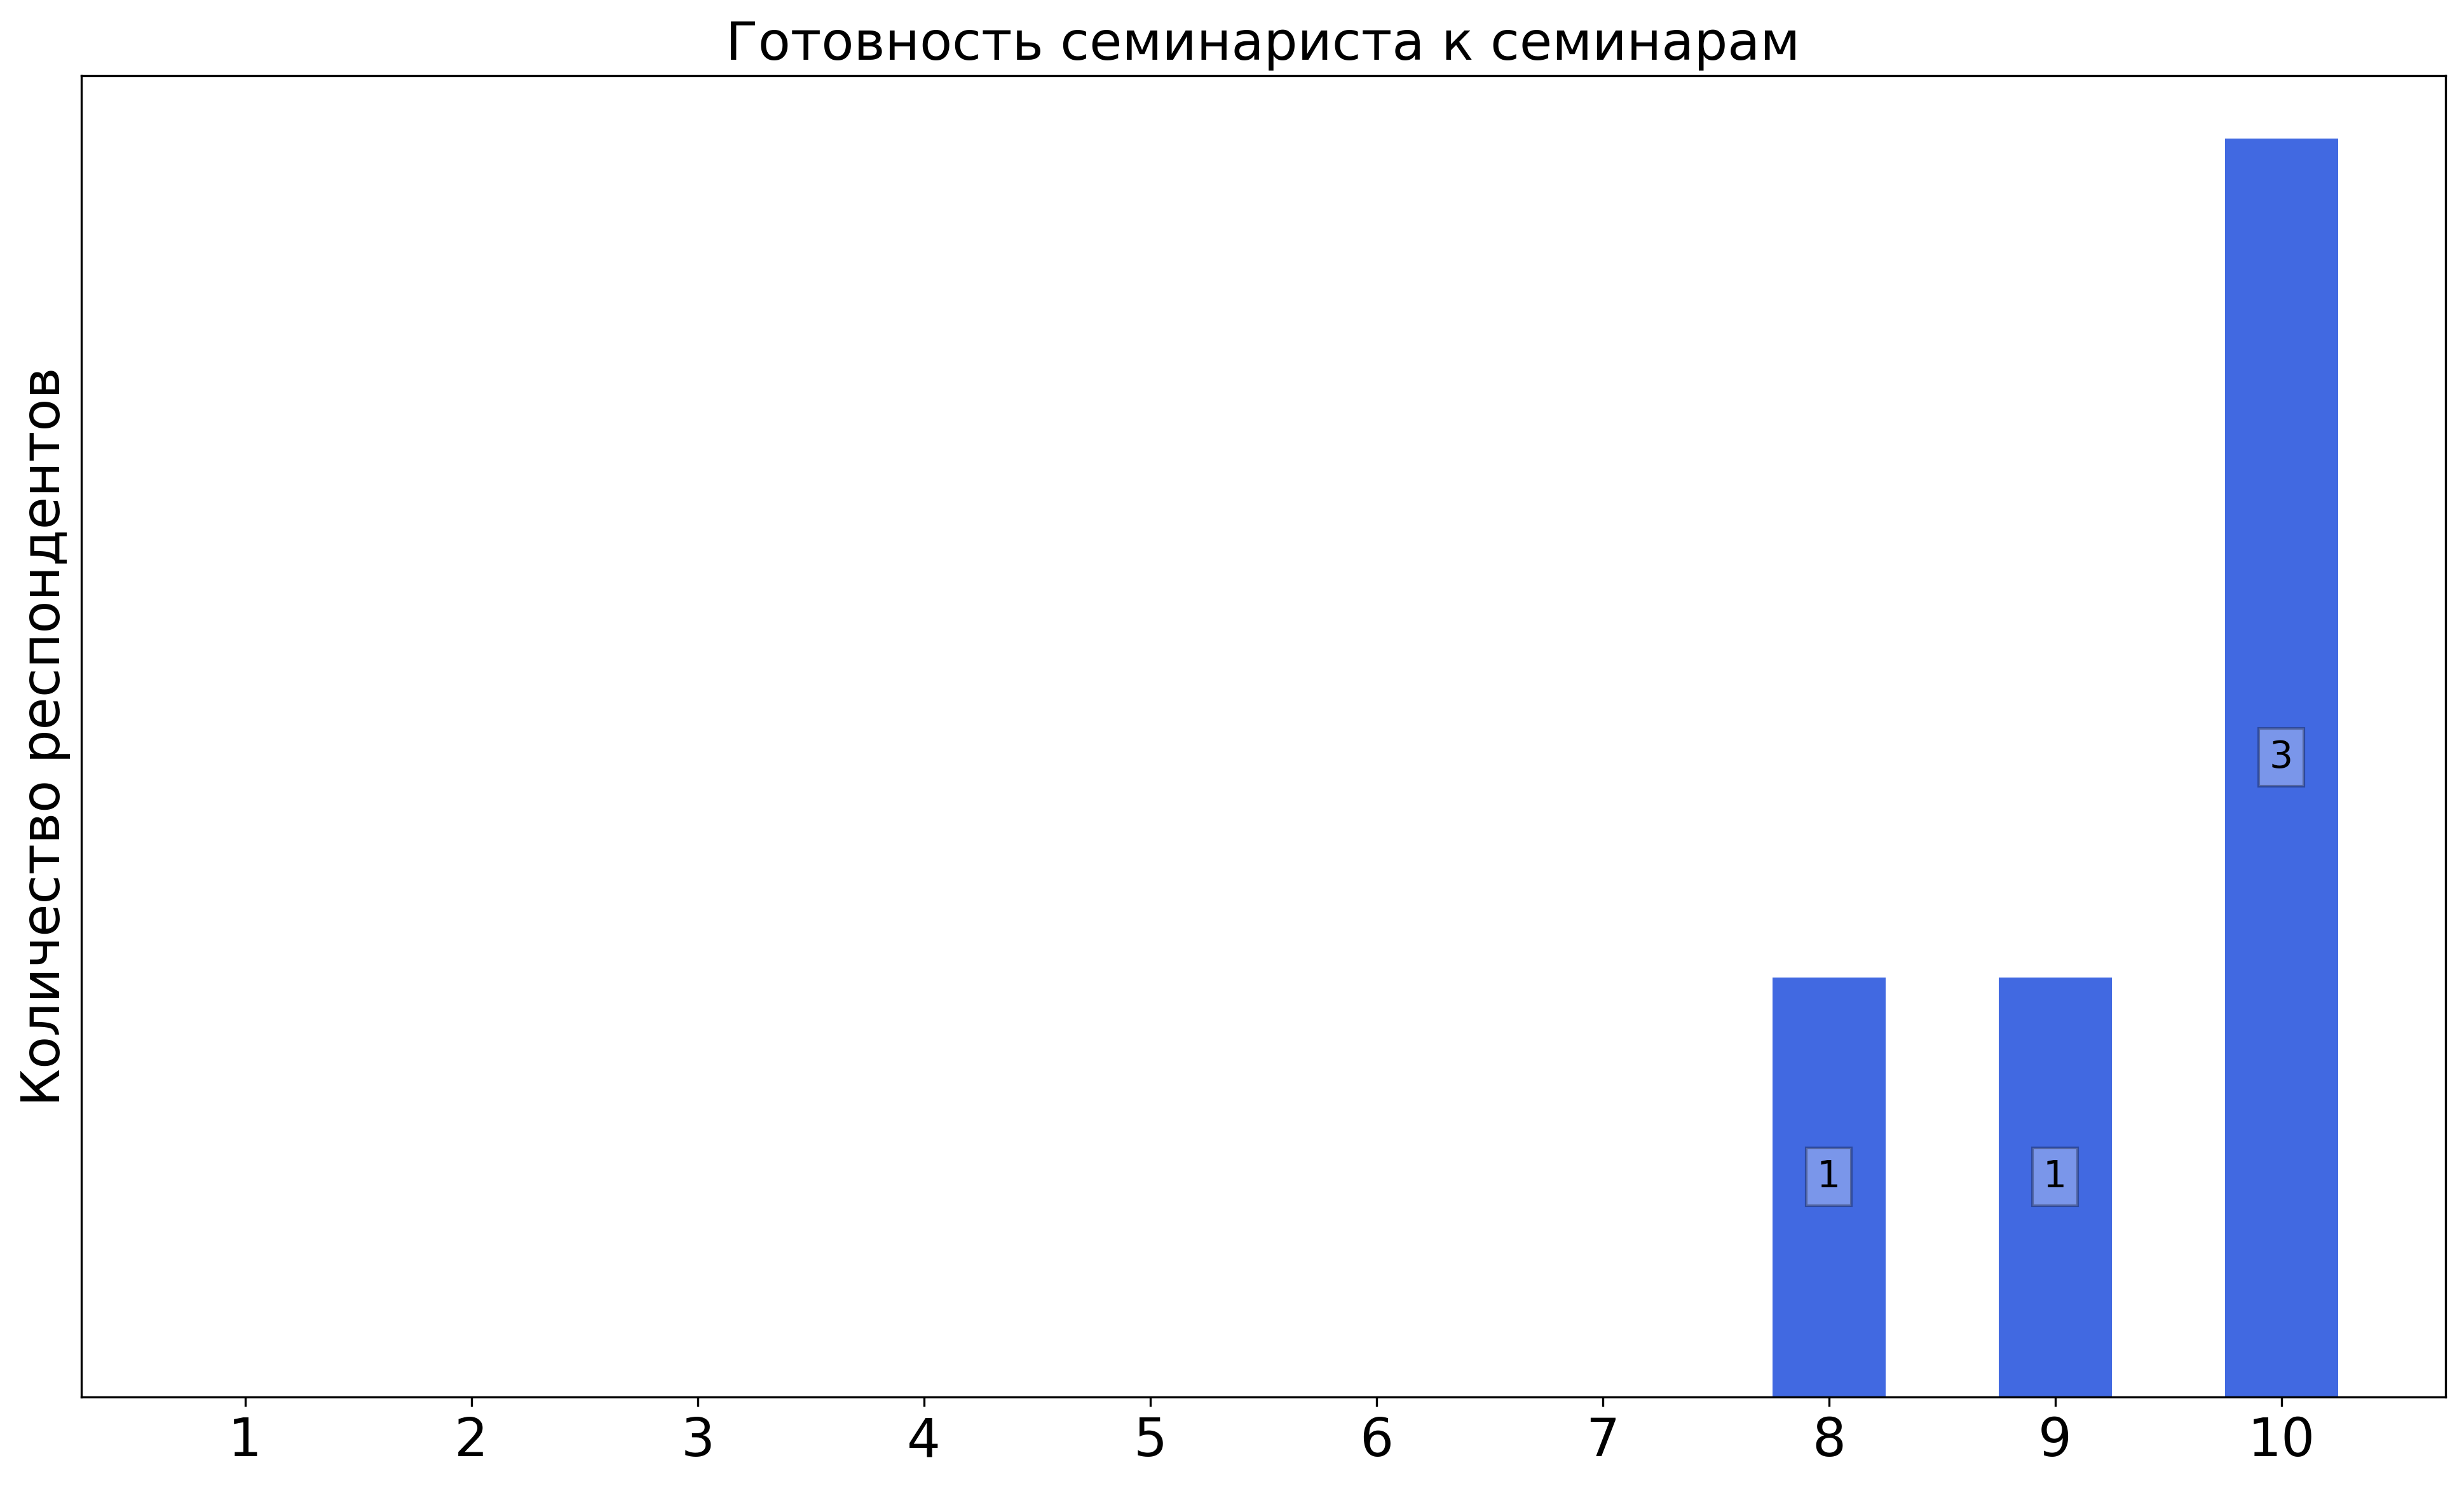
\includegraphics[width=\textwidth]{images/4 course/Защита информации/seminarists-marks-Полешко А.-1.png}
            \end{subfigure}
            \begin{subfigure}[b]{0.45\textwidth}
                \centering
                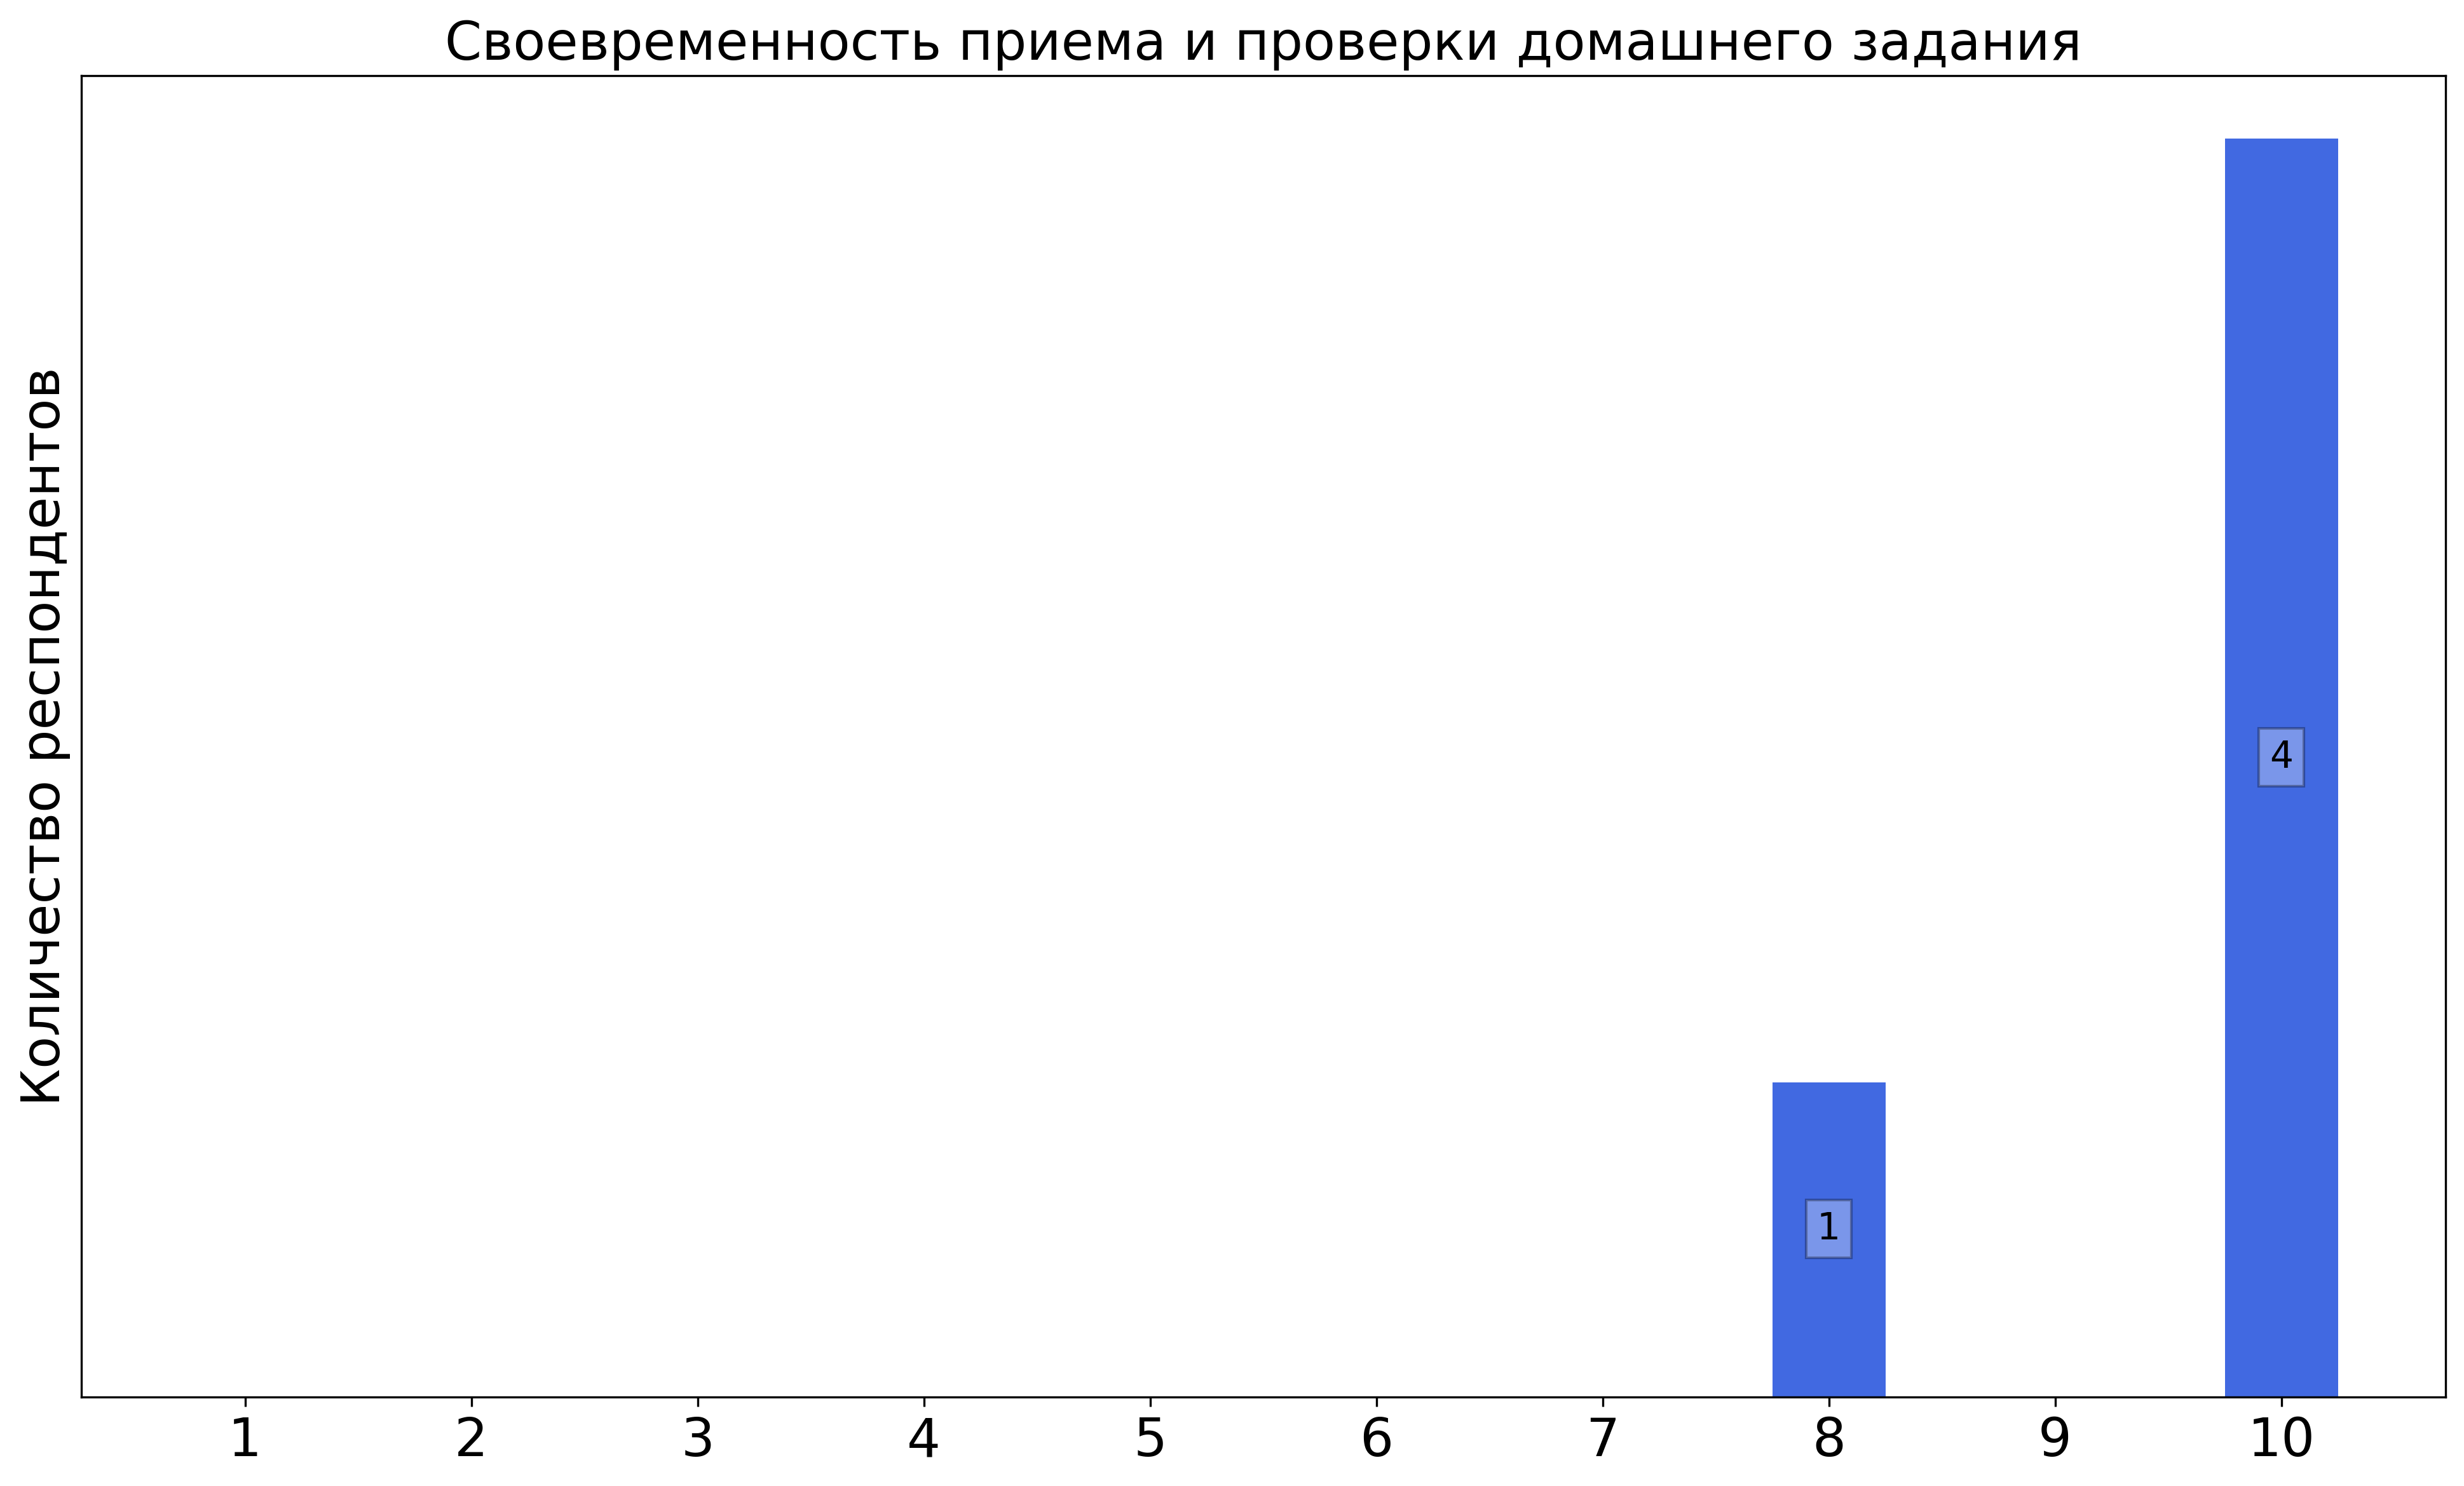
\includegraphics[width=\textwidth]{images/4 course/Защита информации/seminarists-marks-Полешко А.-2.png}
            \end{subfigure}
            \begin{subfigure}[b]{0.45\textwidth}
                \centering
                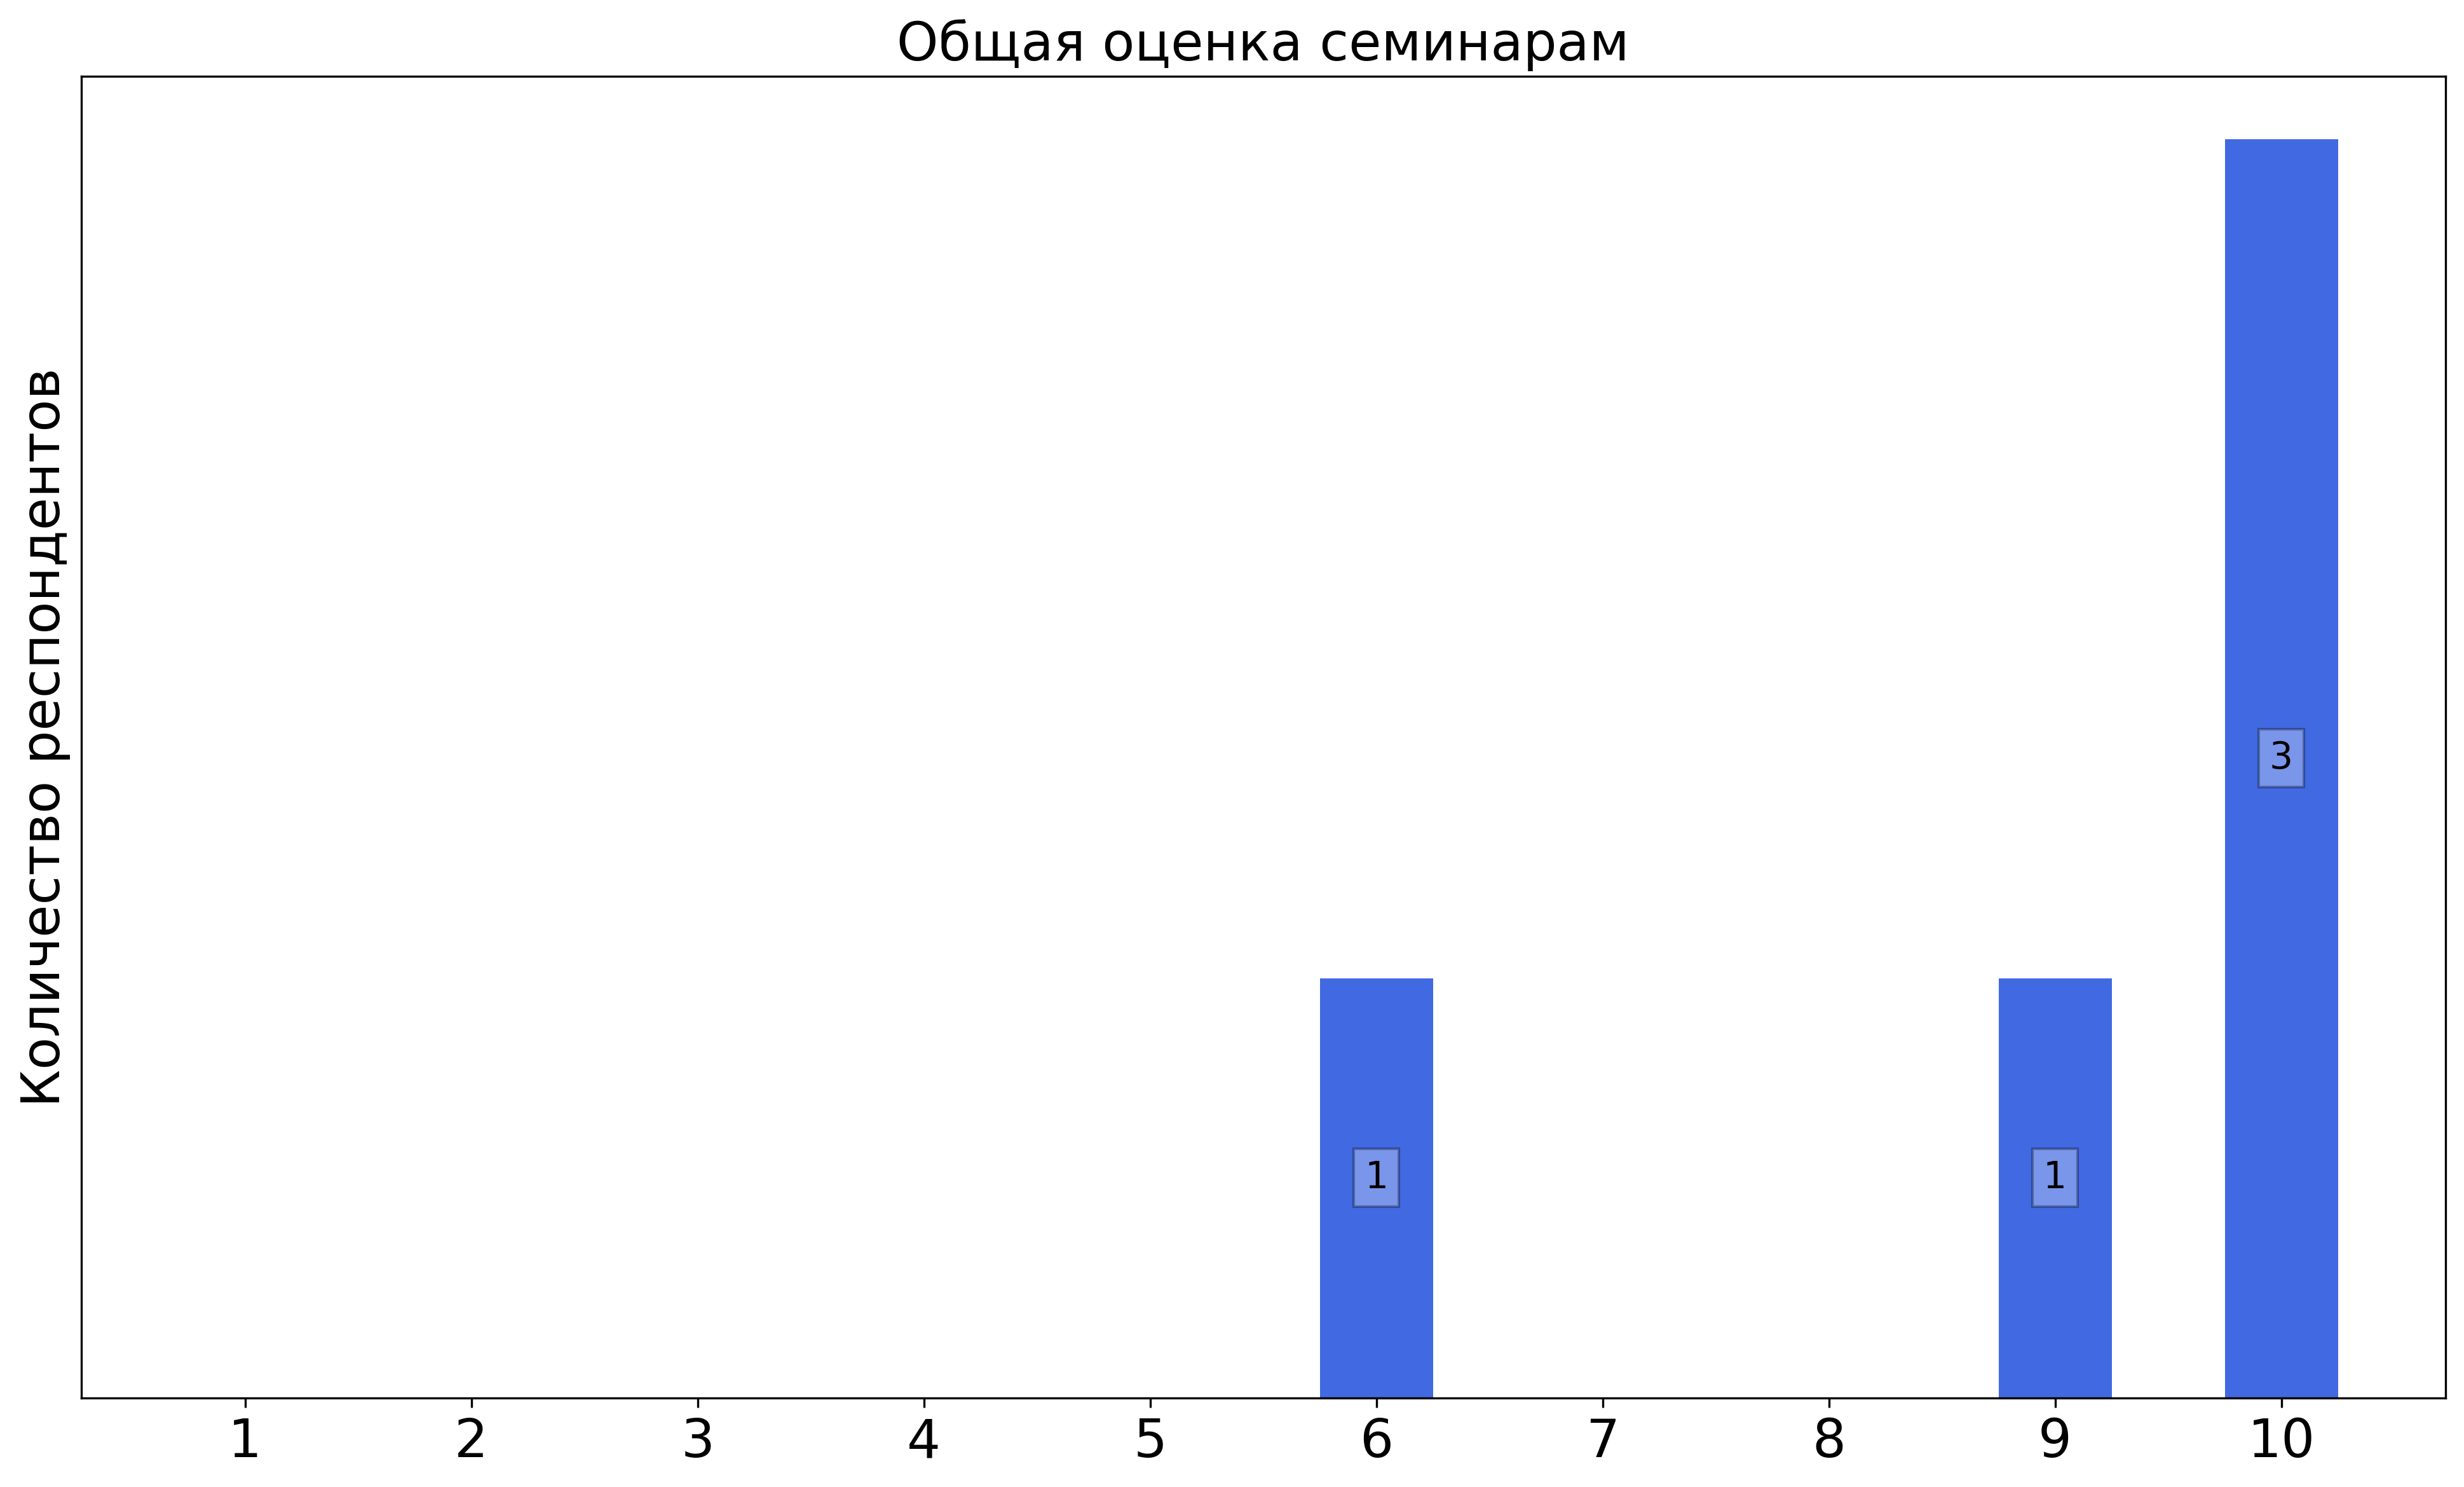
\includegraphics[width=\textwidth]{images/4 course/Защита информации/seminarists-marks-Полешко А.-3.png}
            \end{subfigure}	
            \caption{Оценки респондентов о качестве преподавания семинаров}
        \end{figure}

        \textbf{Комментарии студентов о семинаристе\protect\footnote{сохранены оригинальные орфография и пунктуация}}
            \begin{commentbox} 
                Семинарист хорошая. Ведет семинары с отдачей, отвечает на вопросы, отлично объясняет, приятна в общении.
                Контрольные оценивает адекватно, даёт исправить 
            \end{commentbox} 
        
            \begin{commentbox} 
                Всё было замечательно, удалось найти общий язык 
            \end{commentbox} 
        
            \begin{commentbox} 
                Комментарий не к семинаристу, а к структуре курса. А Полешко красава.
        
                Курс целиком построен на вычислениях чего-то по модулю чего-то. Само по себе это механическое пересчитывание не несёт смысла. Курс можно целиком запрограммировать на компьютере и мы ничего не потеряем. Мне совсем непонятно, зачем нужно было 3 раза писать контрольные по одному и тому же умножению и сложению по модулю.
                
                Проект это хорошо, мне понравилось. 
            \end{commentbox} 

    
    \subsubsection{Прочие комментарии и предложения по улучшению курса}
            \begin{commentbox}
                Не особо понял для чего этот курс вообще, не вижу в нём никакого смысла, так как он ни чему не обучает. Задачи на семинарах и в кр абсолютно типовые и решаются с помощью алгоритма
            \end{commentbox}

            \begin{commentbox}
                Уменьшить количество отчётности для студентов.
            \end{commentbox}

            \begin{commentbox}
                Не знаю как на экзамене но думаю сделать критерии автомата более прозрачными было бы полезно - четко определить баллы с которых он начинается. И может быть пересмотреть эссе как задание и придумать что-то более интересное и не нудное)
            \end{commentbox}

            \begin{commentbox}
                Для более глубокого понимания предмета необходимо изучить курс алгебры, но к сожалению на 4 курсе на это нет времени. Было бы неплохо если бы курс алгебры предшествовал данному курсу
            \end{commentbox}

            \begin{commentbox}
                Его можно было изучить и раньше, особо не было предметов, которые нам нужно было бы изучить до него
            \end{commentbox}

            \begin{commentbox}
                Разрешить пользоваться собственными программами, написанными для расчета  всех этих чисел. Заставить людей показывать историю коммитов, где они писали эту программу, чтобы удостовериться, что она не списана.
            \end{commentbox}
            